\documentclass[a4paper, twoside, openright, 11pt, oldfontcommands]{memoir}
\usepackage[T1]{fontenc}
\usepackage{microtype}
\usepackage{algorithm}
\usepackage{algpseudocode}
\OnehalfSpacing
\usepackage{cite}
\usepackage{amsmath}
\usepackage{mathtools}
\usepackage{amssymb}
\usepackage{subcaption}
\usepackage{fixltx2e}
\usepackage{stmaryrd}
\usepackage{pdfpages}
\usepackage{booktabs}
\usepackage{datetime}
\newdateformat{monthyear}{\monthname[\THEMONTH] \THEYEAR}
\usepackage[pdftex,hyperindex,bookmarks]{hyperref}
\hypersetup{
    pdfborder = {0 0 0.75 [1.5 3]},
    allbordercolors = {0.122 0.471 0.706},
    colorlinks,
    citecolor=black,
    filecolor=black,
    linkcolor=black,
    urlcolor=black
}
\usepackage[authoryear,square]{natbib}
\usepackage{bibentry}
\usepackage{cleveref}
\renewcommand{\cite}{\citep}
\usepackage{tikz}
\usetikzlibrary{arrows.meta,automata,shapes.multipart,positioning,plotmarks}

\let\proof\relax
\let\endproof\relax
\usepackage{amsthm}
\usepackage{xspace}

\algnewcommand{\IIf}[1]{\State\algorithmicif\ #1\ \algorithmicthen}
\algnewcommand{\EndIIf}{}
\algnewcommand{\Continue}{\textbf{continue}}
\algnewcommand{\IfElse}[3]{\algorithmicif\ #1\ \algorithmicthen\ #2\ \algorithmicelse\ #3}
\algnewcommand{\EndIfElse}{}
\algnewcommand{\Break}{\State\textbf{break}}
\algnewcommand{\LineComment}[1]{\State \(\triangleright\) #1}
\MakeRobust{\Call}
\newcommand{\True}{\texttt{true}}
\newcommand{\False}{\texttt{false}}
\newcommand{\II}{\mathcal{I}}
\newcommand{\textoverline}[1]{$\overline{\mbox{#1}}$}

\newcommand{\cS}[0]{\mathcal{S}}
\newcommand{\cU}[0]{\mathcal{U}}
\newcommand{\cC}[0]{\mathcal{C}}
\newcommand{\cSU}[0]{2^{\cS} \times 2^{\cU}}

\newtheorem{example}{Example}
\newtheorem{theorem}{Theorem}
\newtheorem{proposition}{Proposition}

%%% Formatting setup
% 11pt Palatino (URW Palladio) for text
\renewcommand{\rmdefault}{ppl}
% Optima (URW Classico) for headings
%\renewcommand{\sfdefault}{uop}

% Use Courier which has a bold series
\renewcommand{\ttdefault}{pcr}

% Make our pretty chapter headings
% Copied from DaveC via Adam
\usepackage[bf,sf]{titlesec}
\newcommand{\chapformat}[1]{\parbox[c]{0.8\textwidth}{\Huge #1}}
\titleformat{\chapter}[hang]
    {\sffamily\bfseries}
    {\parbox[c]{0.2\textwidth}{\rmfamily\fontsize{72}{72}
     \selectfont\thechapter\hspace{10pt}\rule[-12pt]{2pt}{72pt}}}
    {0pt}
    {\chapformat}

\setsecnumdepth{subsection}

%%%\title{Addressing the Space Explosions of Reactive Synthesis}

%%%\author{Alexander Legg \\
%%%    \\
%%%    Supervised by \\
%%%Leonid Ryzhyk, Nina Narodytska, and Gernot Heiser}

\begin{document}

\nobibliography*

\frontmatter

\thispagestyle{empty}

\calccentering{\unitlength}                         % Calculate center length and stores in unitlength
\begin{adjustwidth*}{\unitlength}{-\unitlength}     % Adjust center
        \begin{adjustwidth}{-1cm}{-1cm}                 % Extra lage front page

\mbox{}
\vfill
\begin{center}
    {\Huge\sffamily\bfseries A Counterexample Guided Method for Reactive Synthesis\\[1cm]\par}
{\Large\sffamily\bfseries Alexander Legg}\\[1.5cm]
Submitted in fulfilment of the requirements for the degree of \\
Doctor of Philosophy\\[1cm]

\includegraphics[width=0.32\linewidth]{unsw-crest-color-smaller} \\[1cm]
School of Computer Science and Engineering \\[0.5cm]
University of New South Wales \\[0.5cm]
Sydney, Australia \\[1.0cm]
\monthyear\today
\end{center}
\par
\vfill

    \end{adjustwidth}
\end{adjustwidth*}

\clearpage

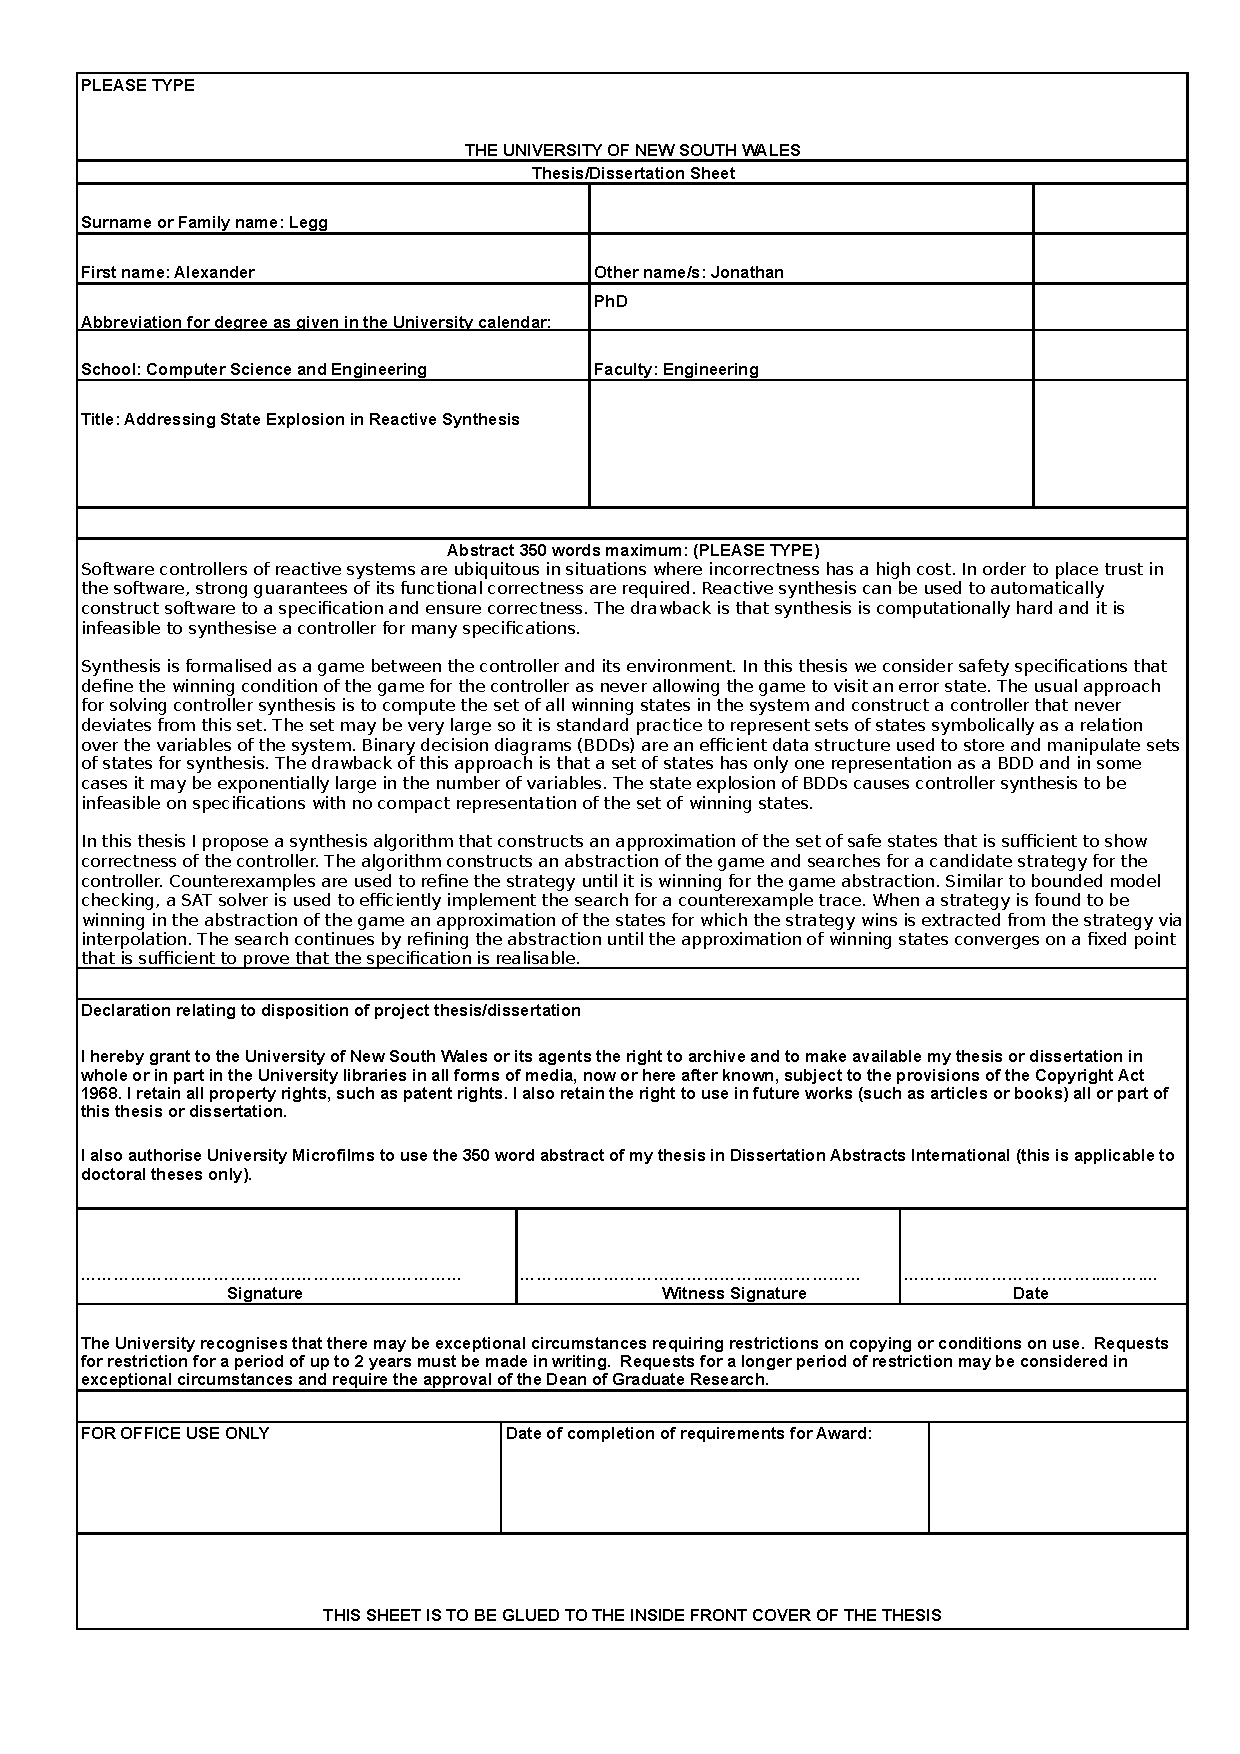
\includepdf{declaration.pdf}

\thispagestyle{plain}
\section*{Originality Statement}
\addcontentsline{toc}{chapter}{Originality Statement}

`I hereby declare that this submission is my own work and to the best of my
knowledge it contains no materials previously published or written by another
person, or substantial proportions of material which have been accepted for
the award of any other degree or diploma at UNSW or any other educational
institution, except where due acknowledgement is made in the thesis. Any
contribution made to the research by others, with whom I have worked at UNSW
or elsewhere, is explicitly acknowledged in the thesis.  I also declare that
the intellectual content of this thesis is the product of my own work, except
to the extent that assistance from others in the project's design and
conception or in style, presentation and linguistic expression is
acknowledged.'\\[0.5cm]
Signed\hspace{0.5cm}\dotfill\hfill\\[0.5cm]
Date\hspace{0.5cm}\dotfill\hfill\\
\vfil\clearpage

\begin{abstract}
    \addcontentsline{toc}{chapter}{Abstract}
Software controllers of reactive systems are ubiquitous in situations where incorrectness has a high cost. In order to place trust in the software, strong guarantees of its functional correctness are required. Reactive synthesis can be used to automatically construct software to a specification and ensure correctness. The drawback is that synthesis is computationally hard and it is infeasible to synthesise a controller for many specifications.

Synthesis is formalised as a game between the controller and its environment. In this thesis we consider safety specifications that define the winning condition of the game for the controller as never allowing the game to visit an error state. The usual approach for solving controller synthesis is to compute the set of all winning states in the system and construct a controller that never deviates from this set. The set may be very large so it is standard practice to represent sets of states symbolically as a relation over the variables of the system. Binary decision diagrams (BDDs) are an efficient data structure used to store and manipulate sets of states for synthesis. The drawback of this approach is that a set of states has only one representation as a BDD and in some cases it may be exponentially large in the number of variables. The state explosion of BDDs causes controller synthesis to be infeasible on specifications with no compact representation of the set of winning states.

In this thesis I propose a synthesis algorithm that constructs an approximation of the set of safe states that is sufficient to show correctness of the controller. The algorithm constructs an abstraction of the game and searches for a candidate strategy for the controller. Counterexamples are used to refine the strategy until it is winning for the game abstraction. Similar to bounded model checking, a SAT solver is used to efficiently implement the search for a counterexample trace. When a strategy is found to be winning in the abstraction of the game an approximation of the states for which the strategy wins is extracted from the strategy via interpolation. The search continues by refining the abstraction until the approximation of winning states converges on a fixed point that is sufficient to prove that the specification is realisable.

\end{abstract}

\newpage

\renewcommand{\abstractname}{Acknowledgements}
\begin{abstract}
Acknowledge some people
\end{abstract}

\chapter{Publications}
\begin{itemize}
    \item \bibentry{Legg16}
    \item \bibentry{Een15}
    \item \bibentry{Narodytska14}
\end{itemize}

\clearpage

\setcounter{secnumdepth}{3}
\setcounter{tocdepth}{3}
\tableofcontents

\newpage

\mainmatter

\chapter{Introduction}

We rely on software systems to perform important tasks for us on a daily basis. Unfortunately we also frequently experience the frustration of an incorrect software system. However, as these systems become more ingrained into our lives the cost of incorrectness can be far greater than mere frustration.

In 1996 the European Space Agency lost their Ariane 5 rocket forty seconds after launch to an incorrect conversion from floating point to integer~\cite{Dowson97}. The cost of the failure was \$370 million in USD. More recently, Toyota has been forced to recall a large number of vehicles due to a failure in the software controlling the brakes~\cite{Parrish13}. The failures led to loss of life~\cite{CBS10}.

As the desire for software and the consequences of incorrectness has grown, the need for a systematic methodology for producing correct software has become apparent. One solution has been to develop strict engineering practices, including rigorous testing, to reduce the chance of errors. Another solution is to produce a proof of correctness of the software, either with or without the aid of a mechanised proof assistant. Model checking can also be used in some cases to automate the correctness proof.

A step further is to have our software automatically constructed for us, a technique first formally considered by Alonzo Church in the middle of the last century~\cite{Church62}. Software synthesis shifts the role of the developer from writing code to writing formal specifications. This completely eradicates the human error factor from the low level construction of software and allows developers to focus on high level system design. In all other approaches to software correctness the software must first be constructed; a process involving considerable time and effort.

Unfortunately, automatic software synthesis involves nontrivial computation. In broad strokes, the synthesis algorithm must determine how the state of the system is affected by the software and its environment and then select actions for the software such that no matter the actions of the environment the system adheres to the specification. In practice, on certain system specifications the process can lead to significant \emph{state explosion} that renders synthesis infeasible.

The state of the art in synthesis contains several methodologies that act as countermeasures to state explosion. However, no single approach is suited to all classes of specifications nor are all specifications currently feasible. In this thesis I propose a methodology for resisting state explosion on a set of synthesis specifications that are problematic for other approaches.

\section{Synthesis}

This thesis is concerned with synthesis of reactive systems. In a reactive system a controller interacts \emph{continuously} with its environment by responding to inputs with the appropriate outputs. For example, a device driver is a reactive system in which the driver interacts with an operating system and a hardware device. Synthesising reactive systems like drivers is different to synthesising regular programs or functions since the correctness of a controller depends on how the system behaves over time instead of a single output corresponding to a single input. As a result, the reactive synthesis problem is staged as a game between the controller and its environment. For a detailed formalisation see Chapter~\ref{ch:background}.

This thesis is concerned with synthesis of controllers for safety games in which the winning condition for the controller is defined by ensuring that the game remains within a set of safe states. The game is zero sum, the environment wins if a state outside the safe set is reached. We say that we have \emph{solved} a game if we can construct a winning strategy for one of the players. The usual approach to solving safety games is to iteratively construct a set of winning states that are known to be safe regardless of the actions of the environment. A winning strategy for the controller can be constructed by choosing actions that have successor states within the winning region.

Explicit enumeration of the states in the winning region is infeasible even on small specifications so the set of states is usually represented symbolically. This is done by specifying the game with states as valuations of a set of boolean variables and using boolean algebra to symbolically define sets of states. Traditionally binary decision diagrams (BDDs) are used to represent boolean functions because they provide compact representations in most cases and there are efficient algorithms for operating on formulas in BDD form. The disadvantage of this approach is that in the worst case the representation occupies space that is exponential in the number of variables in the formula. A BDD is a canonical representation of a formula so it may be the case that a compact BDD representing the winning region for a particular specification does not exist.

Other approaches rely on satisfiability solvers to efficiently perform the operations required by synthesis on sets of states. The satisfiability problem (SAT) is the question of whether a value can be assigned to all variables in a formula such that the formula evaluates to true. Modern SAT solvers provide efficient implementations of backtracking search with computational learning that operate on boolean formulas in clausal normal form (CNF). The advantage of a SAT based approach is that CNF is not canonical so in cases when a BDD cannot compactly represent a set of states it may be possible to do so in CNF.

The disadvantage of SAT based approaches is that solvers only determine whether a satisfying assignment to variables \emph{exists}. This is known as existential quantification. The dual problem, universal quantification, is to determine whether all variable assignments satisfy a formula. Both forms of quantification are required for synthesis in order to decide whether an action exists for one player that satisfies a property for all opponent actions. An example of this kind of computation would be deciding whether the controller can force the game into the winning region regardless of any action the environment chooses. It is possible to perform universal quantification with a SAT solver but it adds considerable complexity, which introduces another bottleneck to the synthesis process.

\section{Approach}

This thesis presents a SAT based approach that computes an approximation of the winning region. By approximating the winning region we hope to avoid the state explosion cost of representing the entire set of winning states. The algorithm is set within a counterexample guided abstraction refinement framework. This is our approach to handling the alternating quantifications of synthesis. Candidate strategies are constructed and refined via counterexamples instead of precisely computing the result of the quantified formula.

In this approach, a SAT solver is used to verify whether a candidate strategy is a winning strategy for a safety game with a fixed number of a game rounds, which we call a bounded game. This approach is similar to bounded model checking where a program is verified by querying a SAT solver for a trace that violates the specification. In our bounded synthesis approach the SAT solver searches for a trace of opponent moves that cause the candidate strategy to lose the bounded game. As with bounded model checking, a counterexample trace informs the algorithm how to refine the candidate strategy.

Discovering a winning strategy for the bounded game does not guarantee that the strategy is winning in the unbounded game. Specifically, if the controller strategy avoids an error state for $k$ rounds the SAT solver cannot guarantee that it can avoid errors for $k+1$ rounds. We address this problem with an extension to the algorithm that iteratively solves bounded games while incrementing the bound. During the execution of the bounded game solver we learn losing states for both players. This computational learning serves a dual purpose by both serving as an optimisation to reduce the search space and also providing the termination condition. By carefully learning states that are losing for the environment we may construct an overapproximation of the environment's winning region. The overapproximation can be used to guarantee that the actual winning region does not contain the initial states and so there cannot be a winning strategy for the environment.


\section{Contribution}

This thesis presents a SAT based counterexample guided approach to controller synthesis of safety specifications. This approach includes a bounded synthesis algorithm, an extension to unbounded synthesis, and a methodology for extracting strategies from the certificate generated by the bounded synthesis algorithm. 

The approach is designed to solve synthesis specifications where the winning region is difficult to represent compactly with existing symbolic techniques. The aim of this work was not to produce a one size fits all approach to safety synthesis but instead to provide a solution suited to problem instances that are difficult to solve for other methods.

The instances that emit winning regions that are difficult to efficiently represent with binary decision diagrams include many real world problems. An example of such a specification is an arbiter that must grant resources from a homogeneous pool in order to fulfil requests from the environment. In this problem the winning region for the environment must exclude all combinations of resource allocations that exceed the number of requests. There is no compact representation of this kind of winning region as a binary decision diagram but in our approach we use overapproximation so that we don't need to find and represent all combinations.

In order to validate the methodology I have implemented the algorithm as an open source tool. In later chapters we present benchmarks that show that the algorithm is promising and although it does not solve as many problem instances as other techniques it performs better on certain classes of problems.


\section{Summary}

\begin{itemize}

    \item \emph{Reactive synthesis} can be used to automatically generate correct-by-construction controllers for software systems. Compared to other approaches to software correctness synthesis does not require the software to first be developed.

    \item Synthesis is formalised as a game between a controller and its environment. In many cases these games can be solved by constructing a symbolic representation of the winning states of the game using a binary decision diagram. However, for some games there is no compact representation of the winning region.

    \item This thesis presents a SAT based counterexample guided approach that targets these cases by constructing an approximation of the winning region that is sufficient to determine the winner of the game.

\end{itemize}


%%%\section{Device Drivers}

%%%Device drivers are the software that allows the operating system to interface
%%%with hardware. The role of the driver is to manipulate the inputs of the device
%%%so that it remains in a error-free state and correctly handles the requests of
%%%the operating system. By way of example consider an ethernet driver. The driver
%%%accepts requests to send and receive data packets from the OS and acts on those
%%%requests by reading from and writing to buffers on the device. It must ensure
%%%that those buffers are maintained in a usable state by correctly updating a
%%%register containing the location of the head of the buffer queue.

%%%According to a study performed in 2011~\cite{Palix11}, drivers account for
%%%approximately 57\% of the lines of code in the Linux kernel and subsequently is
%%%the largest source of bugs. The study also analysed the staging directory of
%%%the kernel, which contains all in-progress drivers, and found it to contain the
%%%highest fault rate (faults per line of code) out of any directory in the
%%%kernel. The results of the study give evidence to the widely held belief that
%%%correct drivers are hard to produce.

%%%Consequences of buggy drivers

%%%This thesis focuses on automatic construction of correct drivers as a solution
%%%to the driver problem. Alternate approaches, of which there are many, will be
%%%discussed in Chapter~\ref{ch:relatedwork}.



\chapter{Background}

This is the background.


\chapter{Related Work}
\label{ch:relatedwork}

Reactive synthesis is an extensively studied topic and the work of this thesis is influenced by a wide array of prior work. In the previous chapter we identified symbolic representation of state sets and abstraction refinement as methodologies for mitigating state explosion. In this chapter we will approach the problem from a different angle. The work in this thesis is inspired by research in the model checking community and some prior efforts to apply that research to synthesis.

\section{Bounded model checking}

Bounded model checking~\cite{Biere99} (BMC), as introduced in Chapter~\ref{sec:boundedmodelchecking}, is a methodology that generates SAT queries to determine the existence of a trace in a game that violates its specification. The approach taken to realisability described in Chapter~\ref{ch:bounded} is inspired by BMC and also unrolls the transition relationship into a SAT query and searches for counterexample traces. 

BMC considers the validity of CTL* formulas in Kripke structures in which the game is bounded to $k$ rounds. The authors of the procedure provide a semantics for the translation of CTL* formulas on bounded models, via LTL, to satisfiability constraints. Consider a safety property $AG \phi$ as an example. A safety property is universal and so is checked in BMC by searching existentially for counterexamples in the form of the negation $F \lnot \phi$. The search is translated into a SAT query by unrolling the transition relation $R$ like so: $s_0 \land \bigwedge_{i=0}^{k-1} R(s_i, s_{i+1})$. The LTL formula is similarly translated into a formula $\bigvee_{i=0}^{k} \lnot \phi \in L(s_i)$. The SAT query is equivalent to a check whether there is a path in the bounded Kripke structure $(s_0, s_1, ..., s_k)$ such that $\lnot \phi$ holds in some state $s_i$.

For bounded realisability, the unrolling of the transition relation and the translation of the safety property can be done in much the same way. The difference is that in a synthesis problem the model has yet to be constructed and the algorithm must be given the freedom to choose the actions of the controller. For more details about how this can be overcome, see Chapter~\ref{ch:bounded}.

One of the motivations behind bounded model checking is aligned with the aim of this thesis: to avoid the high cost in space of approaches that construct a symbolic representation of the winning region as a binary decision diagram. By bounding the length the game the procedure can rely on SAT as a symbolic representation instead of BDDs. The drawback is that although BMC is sound, any counterexample is a true counterexample, it is not complete with respect to the unbounded game unless a sufficient bound is used. For safety properties the diameter of the game gives a tight sufficient upper bound for BMC although it is difficult to compute. Due to the additional complexity of synthesis it is not feasible to use the diameter in a bounded synthesis procedure.

\section{Unbounded model checking}

The usage of SAT solvers in bounded model checking proved to be highly beneficial for discovering counterexamples. Research into applications of SAT in unbounded model checking has subsequently progressed in several directions.

\subsection{Non-canonical symbolic representation}

One approach to unbounded model checking is to replace BDDs with binary expression diagrams (BEDs) or reduced boolean circuits (RBCs) in a fixed point algorithm~\cite{Williams00, Abdulla00}. BEDs are a generalisation of BDDS with the advantage that BEDs are not canonical and their use as a symbolic representation may be more succinct than the equivalent BDD. An RBC is simply a graphical representation of a circuit with some reductions applied. The two representations are essentially orthogonal and conversion between them is linear.

The disadvantage is that the controllable predecessor computations during the fixed point calculation require quantifier elimination that increase the size of the BED or RBC. Detecting a fixed point in the state sets then requires a costly satisfiability check of combinations of the expanded formulas. One option is to construct an equivalent BDD for which the satisfiability check is efficient but potentially negates the advantage of the non-canonical representation. It is also possible to construct a CNF representation of the formula from either a BED or RBC and query a SAT solver for satisfiability. Neither option fully mitigates the potential size of the expanded formula due to quantifier elimination. In practice this methodology works well only on models with few inputs so that quantification does not explode the formulas.

\subsection{Hybrid SAT/BDD approach}

Although many research efforts are directed away from BDDs to avoid their space blowup some work instead focuses on allowing a trade off between space and time via combinations of SAT procedures with BDDs. One such approach~\cite{Gupta00} uses BDDs to enhance SAT in two ways during a reachability fixed point algorithm.In Chapter~\ref{ch:background} a fixed point algorithm for solving safety games using the uncontrollable predecessor backwards from the error set was introduced. The authors of this work solve the dual game, reachability, in a forwards direction by iteratively computing the \emph{image} of the initial states. The image operator takes a set of source states and returns the states that one player can force the game to. This is the forward searching version of the uncontrollable predecessor, which is also sometimes called a \emph{preimage}.

The authors introduce a technique they call \emph{BDD bounding} to prune the search space of the SAT procedure by checking that partial assignments to a set of variables during the SAT search are contained within a BDD. An image computation requires that the assignment to current state variables is contained within the source states computed during the previous iteration. The set of source states may be represented as a BDD and BDD bounding applied to the search in order to detect and immediately backtrack when a satisfying assignment has current state variables set to a value outside the BDD.

It is possible to directly apply SAT to quantifier elimination, and thus to image computation, by repeatedly applying a SAT solver to find all satisfying solutions. This methodology applied without any optimisations is generally infeasible due to the large number of calls that must be made to the SAT solver. The authors of \cite{Gupta00} introduce a middle ground between this entirely SAT based approach and a standard BDD image computation. They suggest interrupting the SAT procedure after some partial assignment has been made to continue computation with a BDD. Effectively this is BDD image computation but distributed into smaller components by the SAT solver.

\subsection{SAT based unbounded model checking}

An optimised approach to SAT image computation is an efficient model checking procedure is cases where cube enumeration does not cause exponential blowup~\cite{McMillan02}. McMillan proposes constructing \emph{blocking clauses} by modifying the SAT procedure and analysing the solver's internal implication graph. The result is effectively cube enumeration that produces a CNF formula with intelligently enlarged cubes so that the original formula is covered in fewer SAT calls. The procedure is applied to CTL model checking by performing universal quantification on CNF formulas via variable deletion.

\subsection{Application of Craig interpolants}

Another angle of research is to extend bounded model checking into an unbounded procedure via a more efficient means than computing a diameter or other sufficient bound. In \cite{McMillan03} Craig interpolation is proposed as means of approximating the set of reachable states during bounded model checking. 

Recall the introduction of Craig interpolants in Section~\ref{sec:backgroundInterpolation}. An interpolant is a formula that may be constructed efficiently from the resolution proof of two mutually unsatisfiable formulas. It is implied by one formula and the conjunction with the second formula is unsatisfiable. During bounded model checking a formula representing an unrolling of the transition relation of length $k$ is unsatisfiable if there is no counterexample trace. This formula may be separated into an initial game round and $k-1$ remaining game rounds enabling a convenient application of interpolation. An interpolant constructed this way is an overapproximation of the image computation on the initial states and the states contained in the interpolant cannot emit a counterexample in $k-1$ game rounds.

This process is applied iteratively by setting the starting point of the unrolled formula to the union of the initial states and any previously computed interpolants. By construction via interpolants no state inside this set enables a counterexample run. Eventually this set will either reach a fixed point and provide an inductive invariant of the system, indicating that the specification of the model holds in the unbounded game, or a counterexample run will be found.

\subsection{Properly Directed Reachability (PDR)}
\label{sec:pdr}

More recently an approach was proposed that solves safety games without unrolling the transition relation of the game~\cite{Bradley11}. The intuition of the algorithm is to construct a proof of a safety properly $P$ by incrementally strengthening a series of inductive lemmas. This procedure provided the inspiration for the unbounded realisability algorithm of Chapter~\ref{ch:unbounded}.

The algorithm maintains a series of formulas $F_0, F_1, ..., F_k$ that overapproximate the set of states reachable in $0, 1, ..., k$ game rounds. The sequence is extended when $F_k \land T \to P'$ is true indicating that $F_{k+1} = P$ is a new reachable set that maintains the safety property. Then clauses in each $F_i$ are propagated forwards to $F_{i+1}$ if it is possible to do so. When $P$ is not reachable from $F_k$ there must be a state within $F_k$ that is one step from violating the safety property. Either this state indicates a counterexample or a new relatively inductive clause can be added to some $F_i$ to prevent the state from being reachable at $F_k$. If during the forward propagation of clauses two formulas $F_i$ and $F_{i+1}$ become equivalent the algorithm has reached a fixed point and has proved that the safety property is invariant.

\section{Synthesis with SAT}

Given the success of model checking techniques employing satisfiability methods it is no surprise that many attempts have been made to replicate these results in the context of synthesis. Synthesis is a significantly more complex problem and it is not obvious how to translate the advantages of SAT, namely the ability to quickly find counterexamples, to an algorithm that must construct a model before checking it. Nonetheless advances have been made that are able to outperform BDD methods in some situations.

\subsection{Bounded Synthesis}

In Chapter~\ref{ch:bounded} we will discuss a bounded realisability algorithm. The bounded synthesis methodology introduced by \cite{Finkbeiner13} is an unfortunate conflation of terms. Their approach places a bound on the size of the implementation as opposed to bounding the length of the game as in Chapter~\ref{ch:bounded} and in bounded model checking. 

This bounded synthesis approach is used to synthesise reactive systems for distributed architectures by first constructing a universal co-B\"uchi automaton for the given LTL specification. An implementation is a transition system that drives that automaton thereby producing a run graph. The run graph of a transition system may be annotated in each node with the maximal number of rejecting states that occur on any path to that node. The authors show that the existence of an annotation with finite bounds indicates that its transition system is accepted by the automaton and hence the LTL specification. A bound is placed on the size of the transition system, which additionally sets an upper bound for the maximum label in the annotation, and an SMT solver can be used to search for a bounded transition system that has a valid annotation. In this way LTL synthesis is reduced to a series of SAT modulo integer arithmetic problems with increasing bounds.

One synthesis tool~\cite{Ehlers12} divides an LTL specification into safety and non-safety components. The safety components are solved easily by a standard symbolic algorithm with BDDs. The author proposes a symbolic version of bounded synthesis to solve the non-safety components. Their approach constructs a BDD that encodes the search for a transition system with a valid annotation. Another approach~\cite{Filiot11} similarly does symbolic bounded synthesis using antichains.

\subsection{Lazy Synthesis}

A counterexample guided framework has been applied to bounded synthesis in a methodology called lazy synthesis~\cite{Finkbeiner12}. The authors propose the construction of bounded size partial implementations via SMT solving a collection of constraints. The partial implementation is then model checked in a symbolic BDD algorithm and any counterexamples are used to introduce new constraints that refine the partial strategy. If the implementation is found to be correct during the model checking phase then the algorithm terminates. Alternatively, the constraint solver may return that there is no implementation at which point the bound on the size of the implementation is increased. 

The counterexample guided search for a correct implementation is similar to the bounded realisability approach proposed in Chapter~\ref{ch:bounded}. The framework is fundamentally the same: candidate strategies are found by a SAT solver, they are checked for correctness, and counterexamples are used to refine further searches for candidates. However, the two methodologies use different approaches to each component of that framework.

\subsection{Properly directed reachability applied to synthesis}

The incremental induction of PDR~\cite{Bradley11} (see Section~\ref{sec:pdr}) has also been applied to the realisability problem. In \cite{Morgenstern13} the authors suggest that by replacing the SAT queries used to approximate reachability with 2QBF queries that the algorithm may be used to solve realisability of safety games. 

Their approach computes overapproximations of the sets of states from which the environment can force to an error state in some number of game rounds. A state is added to the overappoximation of states that are environment winning in $k$ rounds via a 2QBF query that checks whether the environment has an action such that for all controller actions a successor state is inside the overapproximation of states winning in $k-1$ rounds. This generates new obligations for the algorithm to refine the overapproximations. Each successor state must now be checked for the ability for the environment to win in $k-1$ rounds. Eventually this process may discover a chain of states from the initial set to the error set such that the environment can force a win. Alternatively the overapproximating sets will reach a fixed point indicating that the controller can force the game to stay within a set of safe states.

The universal quantification in the 2QBF query is costly to compute so the authors propose repurposing SAT for the task. Similar to how QBFs are solved in \cite{Janota12} and in Chapter~\ref{ch:bounded}, a SAT query checks whether there is an existentially quantified pair of controller and environment actions that reaches the desired set, and another SAT query gives the controller the opportunity to revise its action. Intuitively, the first query \emph{guesses} an environment transition and the second query \emph{checks} it. To assist the process an overapproximation of controller winning states is maintained and used to direct the controller away from its losing states in the checking query. Additionally, the environment transitions that turn out to be bad guesses are learned and blocked in future attempts.

A recent approach~\cite{Chiang15} has a similar application of PDR to synthesis with the major difference being that the authors propose solving the game forwards from the initial states instead of backwards from the error set. Thus the relatively inductive sets represent overapproximations of reachable states. In the previous work the SAT query checks for environment actions that force a successor state into an approximation of environment winning states. As a result, when a transition is found to have a countering controller action it is only known to be a bad transition for the environment to force into the current target. In this more recent work the SAT query is always attempting to find transitions \emph{from} the (approximate) reachable sets into the error set. An advantage of this approach is that learned transitions may be blocked in \emph{all} future queries.

\subsection{Clause Learning for Synthesis}

In \cite{Bloem14} the authors propose a suite of learning algorithms for synthesis. Two of these algorithms are centred on learning unsafe states by solving a quantified formula that checks for environment controllable successor states outside the current approximation of the safe region. When such a state is discovered it is generalised into multiple cubes representing sets of states that are then blocked from the safe region. The specification is decided unrealisable when the initial states are no longer within the safe region and realisable when there are no states left to learn. 

The two variations of this algorithm correspond to one based on a QBF solver and one based on two competing incremental SAT solvers. The latter contains an optimisation to ensure that the incremental nature of the solvers is exploited. Incremental solvers work well in the case where new constraints are added to the problem over time. Removing constraints requires either careful backtracking of learned clauses or restarting the session with no clauses. As the safe region is restricted by blocking cubes the constraints of the solver playing on the behalf of the environment are reduced by enabling the search for transitions to outside the safe region to visit the blocked cubes. The authors suggest maintaining a separate instance of the safe region that is lazily updated. The environment searches for states with successor states outside the old version of the safe region until it is necessary to make the costly update to the incremental solver to the more permissive new safe region.

Another optimisation take inspiration from PDR to approximate reachability information during clause learning. It is not useful to learn unreachable states to remove from the safe region so the search space can be pruned by only considering an overapproximation of reachable states. The optimisation is implemented first by checking candidates for learning for inclusion in the initial set or a predecessor inside the current safe region estimate.

The authors additionally propose two approaches that attempt to directly compute a winning region. The first of these searches for assignments to the parameters of a CNF template of the winning region with a call to a QBF solver. The parameters correspond to the polarity and inclusion of variables within clauses. The second constructs an \emph{effectively propositional logic} (EPR) formula that characterises the Skolem functions encoding the winning region of the game. This cannot be solved via QBF due to the nonlinear nature of quantifiers over current and successor variables that describe the winning region. The formula can be encoded in EPR and handed to an efficient solver.

Each of these algorithms has been implemented in a tool that has the ability to run various combinations in parallel. The authors report a significant benefit to parallelisation and sharing of learned clauses in between algorithms.

\section{Quantified Boolean Formula Solving}

A quantified boolean formula (QBF) generalises the satisfiability problem to include universal and existential quantifiers (see Section~\ref{sec:backgroundQBF}). In accordance with the additional complexity of quantification QBF solvers have so far been less successful than SAT solvers at scaling to real world problems. However recent work in which competing SAT solvers are employed on behalf of each quantifier in a QBF problem have shown promising advances.

The bounded realisability problems of Chapter~\ref{ch:bounded} are specialisations of QBF problems. The algorithm proposed to solve those problems can be seen as a domain specific QBF solver. In particular, the algorithm is similar to and inspired by the general QBF algorithm of \cite{Janota12}. In this section we will review the state of the art in QBF solving in order to shed light on the advantages that an algorithm such as in Chapter~\ref{ch:bounded} has over a generalised QBF solver.

QBFs may be solved by application of DPLL~\cite{Cadoli98} or by \emph{expansion} into SAT~\cite{Ayari02} (see Section~\ref{sec:backgroundQBF}). In the former, which we refer to as \emph{search-based} approaches, computational learning can be applied to share information between separate branches of the search tree~\cite{Zhang02,Giunchiglia02}. In SAT conflicts are be remembered in order to prune the search space but once a satisfying assignment is found the solver may terminate. A QBF solver must explore satisfiability in multiple branches of the search in order to establish truth for every value to universal variables. This additional aspect to search may also be reduced by retaining \emph{cubes} of assignments that are known to lead to satisfiability.

\subsection{Q-resolution}

Q-resolution~\cite{Buning95} is a method for combining clauses and eliminating variables to eventually solve a QBF. We consider QBFs in prenex normal form with quantifiers $Q_1 \hat{x}_1 Q_2 \hat{x}_2 ... Q_n \hat{x}_n$. We assign an ordering to variables corresponding to its scope: $\hat{x}_1 < \hat{x}_2 < ... < \hat{x}_n$. We say that a formula is \emph{forall reduced} if each universally quantified literal $l$ is deleted from clauses with no existentially quantified literals of larger scope. This reduction preserves equivalence and ensures that the innermost quantifier is always existential. For example, $\forall x_1 \exists y_1 \forall x_2  ((x_1 \lor y_1 \lor x_2) \land (x_1 \lor \lnot y_1 \lor \lnot x_2))$ is equivalent to $\forall x_1 \exists y_1 ((x_1 \lor y_1) \land (x_1 \lor \lnot y_1))$.

Q-resolution is used to generate new clauses for a forall reduced QBF. Two existing clauses are selected with opposite polarities of an existentially quantified variable $y$. Taking the union of literals of both clauses, removing $y$ literals, and reapplying forall reduction produces a new clause called the \emph{resolvent}. If all possible resolvent clauses are generated for a variable $y$ it may be removed entirely from the formula along with any clause containing $y$. For example, $\forall x_1 \exists y_1 ((x_1 \lor y_1) \land (x_1 \lor \lnot y_1))$ may be further reduced to $\forall x_1 (x_1)$ by resolving on $y_1$, which after forall reduction is the empty clause and the QBF is shown to be false. 

In practice, solving a QBF with q-resolution alone will generate too many clauses to be feasible. In \cite{Biere05} an approach combining q-resolution with expansion is suggested. Resolution is used to eliminate variables from the innermost existential scope and expansion for the innermost universal scope. A scheduler selects which variable to eliminate next by selecting from all candidate variables the variable with the lowest cost. The cost of eliminating a variable is set to the upper bound of the number of literals introduced to the formula by eliminating that variable.

\subsection{Dependency graphs}

One issue with prenex normal form is that much of the structural information of the original problem is lost on conversion. The quantifier prefix can be seen as a linear variable dependency scheme. In \cite{Lonsing10}, the authors generalise variable dependency to directed acyclic graphs, which is more expressive and may more accurately represent the quantifier structure of the original problem. In a search based solver based on the extension of DPLL to QBF, variables are decided based on the partial ordering defined by the prefix. If the solver instead has access to the more general dependency graph it may have a greater degree of freedom with which to choose the order of decisions and maintain soundness.

Additionally, certain standard optimisations to the search procedure rely on dependency information for correctness. For instance a unit literal is the only unassigned existential literal $l$ in a clause in which all unassigned universal literals are independent to $l$. A unit literal constrains the variable to the polarity of the literal and so decides that variable. With a more expressive dependency scheme it is possible to detect more unit literals and speed up the search.

\subsection{Formula structure}

Structural information about a formula can be used for other optimisations to QBF. Reconstructing a circuit similar to the original problem formulation can lead to a compressed representation and more efficient quantifier elimination~\cite{Pigorsch10, Pigorsch09}. The authors propose an and-inverter graph (AIG) representation and the application of circuit compression techniques such as BDD-sweeping for compression. BDDs may also be used to do quantifier elimination in cases where the representation does not explode. Otherwise quantification is performed directly on the AIG by symbolically expanding the circuit followed by compression.

Circuits may also be used as a representation of the problem in a search-based QBF solver~\cite{Goultiaeva09}. The advantages in this setting include propagation of assignments both forwards and backwards as well as identification of irrelevant \emph{don't care} literals by analysing the gates of a circuit. This technique was further improved by the introduction of ghost literals~\cite{Klieber10}, which enables the solver to propagate cubes of learned satisfying assignments in the same way that learned constraints are.

\subsection{SAT for QBF}

SAT solvers are very efficient at finding satisfying assignment to existential queries but less efficient at proving unsatisfiability or, equivalently, satisfiability of universal queries. This asymmetry has been recognised and turned to an advantage in QBF solvers that use SAT to discover counterexamples to the universal component of QBF problems.

Counterexamples may be used to guide the careful expansion of a QBF~\cite{Janota15} into a propositional formula. This algorithm provides the inspiration for the domain specific QBF solver in \ref{ch:bounded}. The QBF is viewed as a game between an existential player and a universal player in which the existential player attempts to satisfy the formula and the universal player seeks to falsify it. The algorithm solves the game recursively by construction an abstraction, finding a candidate solution for one player under that abstraction, and subsequently verifying that candidate in the concrete game. The game is abstracted by partially expanding the QBF into propositional logic. A subset of possible assignments at each quantifier level are expanded into a disjunction for existential levels or conjunction for universal levels. If the current player cannot win in the abstraction against a restricted opponent then it cannot win in the concrete game so the abstraction can be used to find a candidate valuation to the player's current level variables with an efficient SAT call. The candidate is then checked by recursively calling the solver on the suffix of the formula. This effectively replaces the current player's choice with its candidate selection and hands control to the opponent. If the recursive call discovers a counterexample it is added to the abstraction and a new candidate is found. If there is no counterexample then the current player wins. If the refined abstraction now allows no candidate solution then the opponent wins. The full algorithm is listed in Algorithm~\ref{alg:rareqs}.

\begin{algorithm}
    \begin{algorithmic}[1]
        \Function{solve}{$QX(\varphi)$}
        \If{$\varphi$ has no quantifiers}
            \State \Return $(Q = \exists)$ ? \Call{SAT}{$\varphi$} : \Call{SAT}{$\lnot\varphi$}
        \EndIf
        \State $\omega \gets \emptyset$
        \Loop
        \State $\alpha \gets (Q = \exists)$ ? $\bigwedge_{\mu \in \omega} \varphi[\mu]$ : $\bigvee_{\mu \in \omega} \varphi[\mu]$
        \State $\tau' \gets$ \Call{solve}{\Call{prenex}{$QX(\alpha)$}}
        \IIf{$\tau' = \texttt{NULL}$} \Return $\texttt{NULL}$ \EndIIf
        \State $\tau \gets \{ l\ |\ l \in \tau' \land \texttt{var}(l) \in X \}$
        \State $\mu \gets $ \Call{solve}{$\varphi[\tau]$}
        \IIf{$\mu = \texttt{NULL}$} \Return $\tau$ \EndIIf
        \State $\omega \gets \omega \cup \{ \mu \}$
        \EndLoop
        \EndFunction
    \end{algorithmic}
    \caption{Counterexample guided QBF}
    \label{alg:rareqs}
\end{algorithm}

Two recent counterexample guided approaches work on the idea of abstracting the QBF via the selection of a subset of clauses~\cite{Rabe15,Janota15}. In both works the authors suggest that competing SAT solvers select a subset of clauses for the opposing solver to satisfy at each quantifier alternation. In \cite{Janota12} the QBF abstraction is refined via expansion and may lead to an exponential increase in the size of the formula. By instead linearly increasing the formula to include selection variables enabling an abstraction over clauses the more recent approaches avoid that potential explosion.

An orthogonal approach uses nested SAT solvers to solve formulas of the form $\exists \sigma (\varphi \land (\lnot \exists \tau (\psi)))$ where $\varphi$ is a CNF, $\psi$ is a QBF~\cite{Bogaerts16}. At each quantifier level an underapproximation of $\psi$ is given to a recursive solver while the CNF portion is solved via SAT. The SAT solver hands partial assignments gathered by propagating assignments through $\varphi$ to the nested solvers. The partial assignment is validated on the underapproximation in order to discover conflicts from further inside the QBF. 

\section{Summary}

The bounded realisability algorithm presented in this thesis can be seen as an extension of bounded model checking techniques into synthesis. Bounded realisability replaces the SAT calls in bounded model checking with QBF queries. 
In Chapter~\ref{ch:bounded} I present a domain specific QBF algorithm that solves these queries more efficiently than a generalised QBF solver. In Chaper~\ref{ch:strategy} and Chapter~\ref{ch:unbounded} I present extensions of the bounded realisability algorithm to synthesis and to unbounded games respectively. The approaches of those chapters are similar to existing extensions of bounded model checking into unbounded model checking. In this chapter we reviewed the literature on both bounded and unbounded model checking and the state of the art in QBF solving in order to show the inspirations for the work in this thesis.

This chapter also presented methodologies with a similar aim of applying the efficiency of SAT solving to synthesis. In the following chapters I will present my approach and defer a thorough comparison to the related methodologies until then.


\chapter{Bounded Realisability}
\label{ch:bounded}

\newtheorem*{exmp}{Example}
\newtheorem*{exmpI}{Example: Intuition behind the algorithm}

In this chapter I will describe my work on bounded realisability of reactive systems with safety properties. As introduced in Chapter~\ref{ch:background} reactive realisability is the problem of determining the existence of a program, which we call a \emph{controller}, that continuously interacts with its environment in adherence with a specification. A safety property is a simple correctness condition that lays out a set of states of the system that controller must stay within. In this chapter we will refer to this property in the negation: the controller must avoid \emph{error states}.

Realisability is the first step on the path to synthesis. In the subsequent chapter I will describe an algorithm that extracts the actions of the controller necessary for realisation. This strategy may be used for synthesis: automatic construction of the controller program. Reactive synthesis for controllers with safety properties has many practical uses in areas such as circuit design, device drivers, or industrial automation.

The algorithm described in this chapter solves bounded safety games. Recall that Chapter~\ref{ch:background} introduced games as a formalism for synthesis. In this chapter we are concerned with \emph{bounded} games that restrict all runs to certain length. This concept is borrowed from model checking where it is used for similar aims. Specifically, runs of a bounded game can be checked by a purely propositional formula passed to a SAT solver. The SAT solver provides an efficient method for quickly discovering counterexamples. The algorithm presented here is a counterexample guided abstraction refinement framework that relies on counterexamples to find and refine player strategies.

The primary motivation of this work is to avoid computing the entire set of winning states as would be done in the standard controllable predecessor driven fixpoint algorithm. An explicit representation of the winning set would quickly run into the state explosion issues of synthesis so traditionally the set is represented symbolically with a binary decision diagram. However, a BDD is a canonical representation of a set that, in the worst case, may be exponential in the number of variables. For some systems there is no compact representation of the winning set and for those cases an algorithm that does not compute it, such as the one presented here, is desirable.

\section{Inspiration}

This work draws inspiration from a QBF solving algorithm that treats the QBF problem as a game~\cite{Janota12}. In that algorithm one player assumes the role of the universal quantifiers and the opponent takes on the existential quantifiers. In the game, the players take turns to chooses values for their variables from the outermost quantifier block in. One method of solving QBF games is to expand the formula for each quantified variable by either conjuncting (for universal quantification) or disjuncting (for existential) the formula with the variable set to each possible value. For large QBF instances this expanded formula becomes far too large to solve so the authors introduce abstractions, or partially expanded formulas, to avoid expanding on variables unnecessarily. The abstractions are refined through a CEGAR process of searching for candidate solutions and analysing counterexamples. The full algorithm is described in detail in Chapter~\ref{ch:related}. The bounded synthesis algorithm presented here takes inspiration from the CEGAR framework of this work and can be thought of as a domain specific version of the QBF algorithm.

\section{Algorithm}

\begin{exmp}

We introduce a running example to assist the explanation. We consider a simple
arbiter system in which the environment makes a request for a number of
resources (1 or 2), and the controller may grant access to up to two resources.
The total number of requests grows each round by the number of environment
requests and shrinks by the number of resources granted by the controller in
the previous round.  The controller must ensure that the number of unhandled
requests does not accumulate to more than 2.  Figure~\ref{fig:example} shows
the variables (\ref{fig:examplevars}), the initial state of the system (\ref{fig:exampleinit}), 
and the formulas for computing next-state
variable assignments (\ref{fig:exampletrans}) for this example. We use primed identifiers
to denote next-state variables and curly braces to define the domain of a
variable.

This example is the $n=2$ instance of the more general problem of an arbiter of
$n$ resources. For large values of $n$, the set of winning states has no compact representation, which
makes the problem hard for BDD solvers. In Section~3 we will outline how the
unbounded game can be solved without enumerating all winning states.

\end{exmp}

\begin{figure}
    \begin{subfigure}[t]{\textwidth}
        \centering
        \begin{tabular}{l | l | l}
            \textbf{Controllable} & \textbf{Uncontrollable} & \textbf{State} \\
            \hline
            \texttt{request : \{1, 2\}} & \texttt{grant0 = \{0, 1\}} & \texttt{resource0 = \{0, 1\}} \\
            & \texttt{grant1 : \{0, 1\}} & \texttt{resource1 = \{0, 1\}} \\
            & & \texttt{nrequests : \{0, 1, 2, 3\}} \\
        \end{tabular}
        \caption{Variables}
        \label{fig:examplevars}
    \end{subfigure}

    \begin{subfigure}[t]{\textwidth}
        \centering
        \texttt{resource0 = 0; resource1 = 0; nrequests = 0;}
        \caption{Initial State}
        \label{fig:exampleinit}
    \end{subfigure}

    \begin{subfigure}[t]{\textwidth}
        \begin {align*}
            \texttt{resource0'} & \texttt{ = grant0;} \\
            \texttt{resource1'} & \texttt{ = grant1;} \\
            \texttt{nrequests'} & \texttt{ = (nrequests + request >= resource0 + resource1)} \\ 
                                & \texttt{ ? (nrequests + request - resource0 - resource1) : 0;}
        \end{align*}
        \caption{Transition Relation}
        \label{fig:exampletrans}
    \end{subfigure}
    \caption{Example}
    \label{fig:example}
\end{figure}

Our bounded synthesis algorithm constructs abstractions of the game 
that restrict actions available to one of the players.
Specifically, we consider abstractions represented as trees of actions,
referred to as \emph{abstract game trees} (AGTs).  Figure~\ref{fig:agt} shows
an example abstract game tree restricting the environment (abstract game trees
restricting the controller are similar).  In the abstract game, the controller
can freely choose actions whilst the environment is required to pick actions
from the tree.  After reaching a leaf, the environment continues playing
unrestricted.  The tree in Figure~\ref{fig:agt} restricts the first environment
action to \texttt{request=1}. At the leaf of the tree the game continues
unrestricted.

The root of the tree is annotated by the initial state $s$ of the abstract game
and the bound $k$ on the number of rounds.  We denote $\textsc{nodes}(T)$ the
set of all nodes of a tree $T$, $\textsc{leaves}(T)$ the subset of leaf nodes.
For edge $e$, $\textsc{action}(e)$ is the action that labels the edge, and for
node $n$, $\textsc{height}(k, n)$ is the distance from n to the last round of a
game bounded to $k$ rounds.  $\textsc{height}(k, T)$ is the height of the root
node of the tree.  For node $n$ of the tree, $\textsc{succ}(n)$ is the set of
pairs $\langle e, n' \rangle$ where $n'$ is a child node of $n$ and $e$ is the
edge connecting $n$ and $n'$.

\tikzset{every node/.style={solid}}
\tikzstyle{fixed}=[solid]
\begin{figure}
    \centering
    \captionsetup[subfigure]{width=\textwidth,justification=raggedleft}
    \begin{subfigure}[t]{.2\textwidth}
        \centering
        \begin{minipage}[t][3.8cm][t]{\textwidth}
        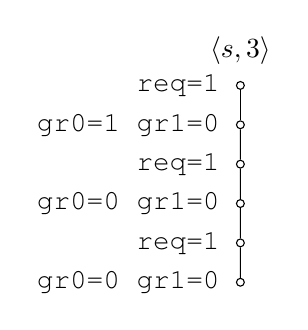
\begin{tikzpicture}[level distance = 5mm,baseline]
            \node [circle,draw,inner sep=1pt] (root){}
                child {node [circle,draw,inner sep=1pt] {}
                    child {node [circle,draw,inner sep=1pt] {}
                        child {node [circle,draw,inner sep=1pt] {}
                            child {node [circle,draw,inner sep=1pt] {}
                                child {node [circle,draw,inner sep=1pt] {}
                                    node [left=4pt] {\texttt{gr0=0 gr1=0}}
                                }
                                node [left=4pt] {\texttt{req=1}}
                            }
                            node [left=4pt] {\texttt{gr0=0 gr1=0}}
                        }
                        node [left=4pt] {\texttt{req=1}}
                    }
                node [left=4pt] {\texttt{gr0=1 gr1=0}}
                }
                node [left=4pt] {\texttt{req=1}}
                node [above=4pt] {$\langle s, 3 \rangle$};
        \end{tikzpicture}
    \end{minipage}
        \caption{Controller winning trace}
        \label{fig:trace}
    \end{subfigure}
    \begin{subfigure}[t]{.2\textwidth}
        \centering
        \begin{minipage}[t][3.8cm][t]{\textwidth}
        \begin{tikzpicture}[dash pattern = on 2pt off 2pt, level distance = 10mm,baseline]
            \node [circle,draw] (root){}
                child {node [circle,draw] {}
                    edge from parent [fixed] node [left] {\texttt{gr0=1 gr1=0}}
                }
                node [left=4pt] {}
                node [above=4pt] {$\langle s, 3 \rangle$};
        \end{tikzpicture}
        \end{minipage}
        \caption{AGT}
        \label{fig:agt}
    \end{subfigure}
    \begin{subfigure}[t]{.2\textwidth}
        \centering
        \begin{minipage}[t][3.8cm][t]{\textwidth}
        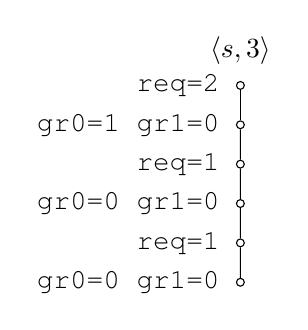
\begin{tikzpicture}[level distance = 5mm,baseline]
            \node [circle,draw,inner sep=1pt] (root){}
                child {node [circle,draw,inner sep=1pt] {}
                    child {node [circle,draw,inner sep=1pt] {}
                        child {node [circle,draw,inner sep=1pt] {}
                            child {node [circle,draw,inner sep=1pt] {}
                                child {node [circle,draw,inner sep=1pt] {}
                                    node [left=4pt] {\texttt{gr0=0 gr1=0}}
                                }
                                node [left=4pt] {\texttt{req=1}}
                            }
                            node [left=4pt] {\texttt{gr0=0 gr1=0}}
                        }
                        node [left=4pt] {\texttt{req=1}}
                    }
                node [left=4pt] {\texttt{gr0=1 gr1=0}}
                }
                node [left=4pt] {\texttt{req=2}}
                node [above=4pt] {$\langle s, 3 \rangle$};
        \end{tikzpicture}
        \end{minipage}
        \caption{Environment winning trace}
        \label{fig:trace2}
    \end{subfigure}
    \begin{subfigure}[t]{.2\textwidth}
        \centering
        \begin{minipage}[t][3.8cm][t]{\textwidth}
        \begin{tikzpicture}[dash pattern = on 2pt off 2pt, level distance = 10mm,baseline]
            \node [circle,draw] (root){}
                child {node [circle,draw] {}
                    edge from parent [fixed] node [left] {\texttt{gr0=1 gr1=0}}
                }
                node [left=4pt] {\texttt{req=2}}
                node [above=4pt] {$\langle s, 3 \rangle$};
        \end{tikzpicture}
        \end{minipage}
        \caption{Partial Strategy}
        \label{fig:strategy}
    \end{subfigure}
    \caption{Abstract game trees.}
    \label{fig:alltrees}
\end{figure}


Given an environment (controller) abstract game tree $T$ a \emph{partial
strategy} $Strat: \textsc{nodes}(T) \rightarrow \mathcal{C}$ ($Strat: \textsc{nodes}(T)
\rightarrow \mathcal{U}$) labels each node of the tree with the controller's
(environment's) action to be played in that node.   Given a partial strategy
$Strat$, we can map each leaf $l$ of the abstract game tree to $\langle
s',i'\rangle=\textsc{outcome}(\langle s, i\rangle, Strat, l)$ obtained by
playing all controllable and uncontrollable actions on the path from the root
to the leaf.  An environment (controller) partial strategy is \emph{winning against $T$} 
if all its outcomes are states that are winning for the environment (controller)
in the concrete game.


%%%Figure~\ref{fig:strategy} shows an example partial strategy for
%%%the controller.  The controller responds to the requests by first granting
%%%access to \texttt{resource1}, then to \texttt{resource0} in the second round.

\begin{exmpI}

    %% Make it clear that this is intuition only
    We present the intuition behind our bounded synthesis method by applying
    its \emph{simplified version} to the running example.  We begin by finding
    a trace of length $k$ (here we consider $k=3$) that is winning for the
    controller, i.e., that starts from the initial state and avoids the error
    set for three game rounds (see Figure~\ref{fig:trace}).  We use a SAT
    solver to find such a trace, precisely as one would do in bounded model
    checking.  Given this trace we make an initial conjecture that any trace
    starting with action \texttt{gr0=1 gr1=0} is winning for the controller.
    This conjecture is captured in the abstract game tree shown in
    Figure~\ref{fig:agt}.  We validate this conjecture by searching for a
    counterexample trace that reaches an error state with the first controller
    action fixed to \texttt{gr0=1 gr1=0}.   Such a trace, that refutes the
    conjecture, is shown in Figure~\ref{fig:trace2}.  In this trace, the
    environment wins by playing \texttt{req=2} in the first round.  This move
    represents the environment's partial strategy against the abstract game
    tree in Figure~\ref{fig:agt}.  This partial strategy is shown in
    Figure~\ref{fig:strategy}.
    
    Next we strengthen the abstract game tree taking this partial strategy into account.
    To this end we again use a SAT solver to find a trace where the contoller
    wins while the environment plays according to the partial strategy.  In the
    resulting trace (Figure~\ref{fig:trace3}), the controller plays \texttt{gr0=1 gr1=1} in
    the second round.  We refine the abstract game tree using this move as
    shown in Figure~\ref{fig:refined1}.  The environment's partial strategy was
    to make two requests in the first round, to which the controller responds
    by now granting an additional two resources in the second round.

    When the controller cannot refine the tree by extending existing branches,
    it backtracks and creates new branches. Eventually, we obtain the abstract
    game tree shown in Figure~\ref{fig:refined2} for which there does not exist
    a winning partial strategy on behalf of the environment.  We conclude that
    the bounded game is winning for the controller.

\end{exmpI}

\begin{figure}
    \centering
    \begin{subfigure}[t]{.2\textwidth}
        \centering
        \begin{minipage}[t][3.8cm][t]{\textwidth}
        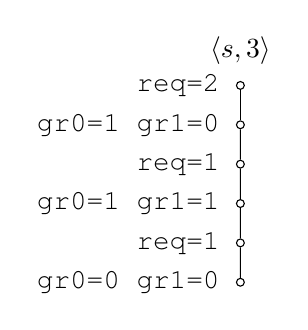
\begin{tikzpicture}[level distance = 5mm,baseline]
            \node [circle,draw,inner sep=1pt] (root){}
                child {node [circle,draw,inner sep=1pt] {}
                    child {node [circle,draw,inner sep=1pt] {}
                        child {node [circle,draw,inner sep=1pt] {}
                            child {node [circle,draw,inner sep=1pt] {}
                                child {node [circle,draw,inner sep=1pt] {}
                                    node [left=4pt] {\texttt{gr0=0 gr1=0}}
                                }
                                node [left=4pt] {\texttt{req=1}}
                            }
                            node [left=4pt] {\texttt{gr0=1 gr1=1}}
                        }
                        node [left=4pt] {\texttt{req=1}}
                    }
                node [left=4pt] {\texttt{gr0=1 gr1=0}}
                }
                node [left=4pt] {\texttt{req=2}}
                node [above=4pt] {$\langle s, 3 \rangle$};
        \end{tikzpicture}
        \end{minipage}
        \caption{Controller winning trace}
        \label{fig:trace3}
    \end{subfigure}
    \begin{subfigure}[t]{.3\textwidth}
        \centering
        \begin{minipage}[t][3.8cm][t]{\textwidth}
        \hspace*{0.8cm}
        \begin{tikzpicture}[dash pattern = on 2pt off 2pt, level distance = 10mm,baseline]
            \node [circle,draw] (root){}
                child {node [circle,draw] {}
                    child {node [circle,draw] {}
                        edge from parent [fixed] node [left] {\texttt{gr0=1 gr1=1}}
                    }
                    edge from parent [fixed] node [left] {\texttt{gr0=1 gr1=0}}
                }
                node [above=4pt] {$\langle s, 3 \rangle$};
        \end{tikzpicture}
        \end{minipage}
        \caption{First refined AGT}
        \label{fig:refined1}
    \end{subfigure}
    \begin{subfigure}[t]{.4\textwidth}
        \centering
        \begin{minipage}[t][3.8cm][t]{\textwidth}
        \begin{tikzpicture}[dash pattern = on 2pt off 2pt, level distance = 10mm,baseline]
            \node [circle,draw] (root){}
                child {node [circle,draw] {}
                    child {node [circle,draw] {}
                        child {node [circle,draw] {}
                            edge from parent [fixed] node [left] {\texttt{gr0=1 gr1=1}}
                        }
                        edge from parent [fixed] node [left] {\texttt{gr0=1 gr1=1}}
                    }
                    edge from parent [fixed] node [left] {\texttt{gr0=1 gr1=0}}
                }
                child {node [circle,draw] {}
                    child {node [circle,draw] {}
                        child {node [circle,draw] {}
                            edge from parent [fixed] node [right] {\texttt{gr0=1 gr1=1}}
                        }
                        edge from parent [fixed] node [right] {\texttt{gr0=1 gr1=1}}
                    }
                    edge from parent [fixed] node [right] {\texttt{gr0=1 gr1=1}}
                }
                node [above=4pt] {$\langle s, 3 \rangle$};
        \end{tikzpicture}
        \end{minipage}
        \caption{Final Refined AGT}
        \label{fig:refined2}
    \end{subfigure}
    \caption{Refined abstract game trees.}
    \label{fig:refinedtrees}
\end{figure}


\begin{algorithm}[t]
    \begin{algorithmic}[1]
        \Function{solveAbstract}{$p, s, k, T$}
        \State $cand \gets $ \Call{findCandidate}{$p, s, k, T$} \Comment{Look for a candidate}
        \IIf{$k = 1$} \Return $cand$ \EndIIf \Comment{Reached the bound}
        \State $T' \gets T$
        \Loop
            \IIf{$cand = \texttt{NULL}$} \Return $\texttt{NULL}$ \EndIIf \Comment{No candidate: return with no solution}
            \State $\langle cex, l, u \rangle \gets $ \Call{verify}{$p, s, k, T, cand$} \Comment{Verify candidate}
            \IIf{$cex = \False$} \Return $cand$ \EndIIf \Comment{No counterexample: return candidate}
            \State $T' \gets $ \Call{append}{$T', l, u$} \Comment{Refine $T'$ with counterexample}
            \State $cand \gets $ \Call{solveAbstract}{$p, s, k, T'$} \Comment{Solve refined game tree}
        \EndLoop
        \EndFunction
        \algstore{b1}
    \end{algorithmic}

    \begin{algorithmic}
        \algrestore{b1}
        \Function{findCandidate}{$p, s, k, T$}
        \State $\hat{T} \gets $ \Call{extend}{$T$} \Comment{Extend the tree with unfixed actions}
            \State $f \gets $ \IfElse{$p = \texttt{cont}$}{\Call{treeFormula}{$k, \hat{T}$}}{\Call{\textoverline{treeFormula}}{$k, \hat{T}$}} \EndIfElse
            \State $sol \gets $ \Call{SAT}{$s(X_{\hat{T}}) \land f$}
            \If{$sol = \texttt{unsat}$} 
                \If{\texttt{unbounded}} \Comment{Active only in the unbounded solver}
                    %\State $\sigma \gets $ \Call{generalise}{$s$} \Comment{Expand $s$ to a set of states}
                    \State \IfElse{$p = \texttt{cont}$}{\Call{learn}{$s, \hat{T}$}}{\Call{\textoverline{learn}}{$s, \hat{T}$}} \EndIfElse
                \EndIf
                \State \Return $\texttt{NULL}$ \Comment{No candidate exists}
            \Else
                \State \Return $\{ \langle n, c \rangle | n \in $ \Call{nodes}{$T$} $, c = \Call{sol}{n} \}$ \Comment{Fix candidate moves in $T$}
            \EndIf
        \EndFunction
        \algstore{b2}
    \end{algorithmic}

    \begin{algorithmic}
        \algrestore{b2}
        \Function{verify}{$p, s, k, T, cand$}
            \For{$l \in leaves(gt)$}
            \State $\langle k', s'\rangle \gets $ \Call{outcome}{$s, k, cand, l$} \Comment{Get bound and state at leaf}
                \State $u \gets $ \Call{solveAbstract}{\Call{opponent}{$p$}, $s'$, $k'$, $\emptyset$} \Comment{Solve for the opponent}
                \IIf{$u \neq \texttt{NULL}$} \Return $\langle \True, l, u \rangle$ \EndIIf \Comment{Return counterexample}
            \EndFor
            \State \Return $\langle \False, \emptyset, \emptyset \rangle$
        \EndFunction
    \end{algorithmic}

    \caption{Bounded synthesis}
    \label{alg:bounded}
\end{algorithm}

The full bounded synthesis algorithm is more complicated: upon finding a candidate 
partial strategy on behalf of player $p$ against abstract game tree $T$, it first checks whether the strategy is winning 
against $T$.  By only considering such strong candidates, we reduce the number of 
refinements needed to solve the game.  To this end, the algorithm checks whether each 
outcome of the candidate strategy is a winning state for $\textsc{opponent}(p)$ by recursively 
invoking the synthesis algorithm on behalf of the opponent.  Thus, our bounded
synthesis algorithm can be seen as running two competing solvers, for the
controller and for the environment. 

%The solvers build candidate partial strategy 
%for their corresponding players, which are used to refine the abstractions.


The full procedure is illustrated in Algorithm~\ref{alg:bounded}.  The
algorithm takes a concrete game $G$ with maximum bound $\kappa$ as an implicit
argument.  In addition, it takes a player $p$ (controller or environment),
state $s$, bound $k$ and an abstract game tree $T$ and returns a winning
partial strategy for $p$, if one exists.  The initial invocation of the
algorithm takes the initial state $I$, bound $\kappa$ and an empty abstract
game tree $\emptyset$.  Initially the solver is playing on behalf of the
environment since that player takes the first move in every game round.  The
empty game tree does not constrain opponent moves, hence solving such an
abstraction is equivalent to solving the original concrete game.

The algorithm is organised as a counterexample-guided abstraction refinement
(CEGAR) loop.  The first step of the algorithm uses the \textsc{findCandidate}
function, described below, to come up with a candidate partial strategy that is
winning when the opponent is restricted to $T$.  If it fails to find a
strategy, this means that no winning partial strategy exists against the opponent
playing according to $T$.  If, on the other hand, a
candidate partial strategy is found, we need to verify if it is indeed winning
for the abstract game $T$.

The \textsc{verify} procedure searches for a \emph{spoiling} counterexample
strategy in each leaf of the candidate partial strategy by calling
\textsc{solveAbstract} for the opponent. The dual solver solves games on behalf
of the opponent player.  

If the dual solver can find no spoiling strategy at any of the leaves, then the
candidate partial strategy is a winning one. Otherwise, \textsc{verify} returns
the move used by the opponent to defeat a leaf of the partial strategy, which
is appended to the corresponding node in $T$ in order to refine it in line~(9).

We solve the refined game by recursively invoking \textsc{solveAbstract} on it.
If no partial winning strategy is found for the refined game then there is also
no partial winning strategy for the original abstract game, and the algorithm
returns a failure.  Otherwise, the partial strategy for the refined game is
\emph{projected} on the original abstract game by removing the leaves
introduced by refinements. The resulting partial strategy becomes a candidate
strategy to be verified at the next iteration of the loop. In the worst case
the loop terminates after all actions in the game are refined into the abstract
game.

The CEGAR loop depends on the ability to guess candidate partial strategies in
\textsc{findCandidate}. For this purpose we use the heuristic that a partial
strategy may be winning if each \textsc{outcome} of the strategy can be
extended to a run of the game that is winning for the current player.  Clearly,
if such a partial strategy does not exist then no winning partial strategy can
exist for the abstract game tree. We can formulate this heuristic as a SAT
query, which is constructed recursively by $\textsc{treeFormula}$ (for the
controller) or $\textsc{\textoverline{treeFormula}}$ (for the environment) in
Algorithm~\ref{alg:treeFormula}.

The tree is first extended to the maximum bound with edges that are labeled
with arbitrary opponent actions (Algorithm~\ref{alg:bounded}, line 14).  For
each node in the tree, new SAT variables are introduced corresponding to the
state ($X_T$) and action ($U_T$ or $C_T$) variables of that node. Additional
variables for the opponent actions in the edges of $T$ are introduced ($U_e$ or
$C_e$) and set to $\textsc{action}(e)$.  The state and action variables of node
$n$ are connected to successor nodes $\textsc{succ}(n)$ by an encoding of the
transition relation and constrained to the winning condition of the player.

%%%Then copies of state and action variables are introduced for each node in the
%%%tree and opponent action variables for each edge $e$ are set to
%%%$\textsc{action}(e)$. 

%%%Candidates are discovered by passing a formulation of the abstract game tree to
%%%a SAT solver in $\textsc{findCandidate}$. This formula contains CNF encodings
%%%of all of the unrolled runs represented by the tree and the winning condition
%%%of the current player.  Runs are encoded by copying the transition relation for
%%%every step in the abstract game. When playing for the controller, the SAT
%%%solver searches for a satisfying assignment to the unfixed label variables in
%%%tree so that none of the runs reaches the error state. The environment
%%%formulation is satisfiable if any run does reach the error state.  The formula
%%%is constructed recursively from the root of a tree by $\textsc{treeFormula}$
%%%(see Algorithm~\ref{alg:treeFormula}).

%%%Since the game tree formulation is passed to a SAT solver, both controllable
%%%and uncontrollable unfixed labels will be existentially quantified. This means
%%%that the SAT solver will find any way to win the game while both players are
%%%cooperating. If no winning run exists in an abstract game even when the players
%%%are cooperating then there is no winning run when the opponent is playing
%%%adversarily. When a winning run is found, the actions chosen by the SAT solver
%%%are used to refine the game tree. This is advantageous for many synthesis
%%%problems where the game must be formalised as adversarial for correctness but
%%%the final implementation will cooperate with its environment in the real world.
%%%An example of such a system is a device driver that cooperates with the device
%%%and OS to provide the interface between the two.

\begin{algorithm}
    \caption{Tree formulas for Controller and Environment respectively}
    \label{alg:treeFormula}
    \begin{algorithmic}[1]
        \Function{treeFormula}{$k, T$}
        \If{$\Call{height}{k, T} = 0$}
        \State \Return{ $\lnot \Call{E}{X_{T}}$ }
        \Else
        \State \Return{$\lnot \Call{E}{X_{T}} \land$ \\
            $$\bigwedge_{\langle e, n \rangle \in \Call{succ}{T}}(\Call{$\delta$}{X_T, U_e, C_T, X_n} \land U_e = \Call{action}{e} \land \Call{treeFormula}{k, n})$$
        }
        \EndIf
        \EndFunction
        \algstore{tf1}
    \end{algorithmic}

    \begin{algorithmic}[1]
        \algrestore{tf1}
        \Function{\textoverline{treeFormula}}{$k, T$}
        \If{$\Call{height}{k, T} = 0$}
        \State \Return{\Call{E}{$X_{T}$}}
        \Else
        \State \Return{ $\Call{E}{X_{T}} \lor$ \\
        $$\bigvee_{\langle e, n \rangle \in \Call{succ}{T}}(\Call{$\delta$}{X_T, U_T, C_e, X_n} \land C_e = \Call{action}{e} \land \Call{\textoverline{treeFormula}}{k, n})$$ }
        \EndIf
        \EndFunction
    \end{algorithmic}
\end{algorithm}

\section{Optimisations}

In this section we present several optimisations to the algorithm.

\subsection{Bad State Learning}

The most important optimisation that allows the algorithm to avoid much of the search space is to record states that are known to be losing for one player. On subsequent calls to the SAT solver we encode these states in the candidate strategy formula (see Algorithm~\ref{alg:treeFormulaLearning}). Thus the algorithm avoids choosing moves that lead to states that are already known to be losing.

Bad states are learned from failed attempts to find a candidate. If the SAT solver cannot find a candidate strategy for a given abstract game tree that means that there is a fixed prefix in the game tree for which the current player can never win. The state reached by playing the moves in the prefix must then be a losing state with some caveats. If the state is at the node with height $k$ and losing for the environment then we know that the environment cannot force to the error set in $k$ rounds. We do not know if the environment can force to the error set in $> k$ rounds. Therefore we record losing states for the environment in an array of sets of states $B^e$ indexed by the height at which the set is losing. For the controller, a losing state is losing for any run of length $>= k$. In practical use we are uninterested in controller strategies that make use of states that would lose should the game be extended to a longer bound so we merely maintain a single set of controller losing states $B^c$.

Additional states can be learned by expanding a single state into a set of losing states by greedily testing each variable of the state for inclusion in a \emph{cube} of states. This technique is well known in the literature and can be efficiently implemented using a SAT solver capable of solving under assumptions~\cite{Een03}. It is shown in Algorithm~\ref{alg:boundedLearning}.

\begin{algorithm}
    \caption{Modified Tree Formulas with Bad State Avoidance}
    \label{alg:treeFormulaLearning}
    \begin{algorithmic}[1]
        \Function{treeFormula}{$k, T$}
        \If{$\Call{height}{k, T} = 0$}
        \State \Return{ $\lnot \Call{E}{X_{T}}$ }
        \Else
        \State \Return{$\lnot \Call{E}{X_{T}} \land$ \\
            $$\bigwedge_{\langle e, n \rangle \in \Call{succ}{T}}(\Call{$\delta$}{X_T, U_e, C_T, X_n} \land U_e = \Call{action}{e} \land \Call{treeFormula}{k, n})$$
        }
        \EndIf
        \EndFunction
        \algstore{tf1}
    \end{algorithmic}

    \begin{algorithmic}[1]
        \algrestore{tf1}
        \Function{\textoverline{treeFormula}}{$k, T$}
        \If{$\Call{height}{k, T} = 0$}
        \State \Return{\Call{E}{$X_{T}$}}
        \Else
        \State \Return{ $\Call{E}{X_{T}} \lor$ \\
        $$\bigvee_{\langle e, n \rangle \in \Call{succ}{T}}(\Call{$\delta$}{X_T, U_T, C_e, X_n} \land C_e = \Call{action}{e} \land \Call{\textoverline{treeFormula}}{k, n})$$ }
        \EndIf
        \EndFunction
    \end{algorithmic}
\end{algorithm}

\subsection{Strategy Shortening}

Learning new bad states means reducing the search space for the algorithm. It follows that it is better to learn states earlier in the algorithm's execution. One problem with relying on SAT calls that assume cooperation is that there is no urgency to the returned candidate strategies. Consider the running example: the environment can reach the error set by setting \texttt{request} to 2 during two rounds. However, in the empty abstract game tree of a bounded game of length 3 or longer, there is no reason for the SAT solver to make the first action one of the requesting rounds if it can assume the environment will never grant any resources. The first action is important because the candidate strategy is derived from that. The candidate is what the opponent has the chance to respond to, so if the candidate does not do anything useful the opponent's response has the freedom to be equally apathetic about reaching its goal. This leads to much of the search space being explored unnecessarily until we learn a losing state.

Encouraging the SAT solver to find \emph{shorter} strategies is a successful heuristic for mitigating this issue. Whilst it does require more SAT calls per call to \textsc{findCandidate} it can be efficiently implemented using incremental SAT solving and during our benchmarking we found the cost to be worthwhile. A strategy is shorter if following the strategy leads to a known bad state for the opponent is fewer game rounds. For the environment this is clearly analogous to reaching the error set sooner. For the controller it is less clear but intuitively states that are environment losing at a certain height are more likely to be \emph{safe} states from which the controller may be able to force a loop.

\subsection{Default Actions}

During the search for a candidate strategy the SAT solver selects actions for the opponent as though the players are cooperating. Sometimes the result is an action that will always fail for the opponent. In many specifications the environment is given the option to fail as a way of modelling errors. For example, in a network driver specification error transitions may be used to model failed connections. When such a transition exists it will often be selected by the SAT solver (especially when the strategy shortening optimisation is enabled). Constantly selecting a bad action for the opponent significantly affects the performance of the algorithm because no bad states can be learned and the solver must refine the game abstraction to avoid the bad action. Additionally, if a candidate strategy was found by relying on a bad action then it will usually need to be backtracked. 

To avoid problematic action selection the solver can instead use some heuristic to select the arbitrary action required in the SAT call in \textsc{findCandidate}. This does not affect the correctness of the algorithm. If no candidate can be found with the opponent playing an arbitrary action then clearly the selected action (or a different opponent action that is winning) would have eventually been refined into the abstract game if the opponent instead cooperated. A simple action selection heuristic has been observed to improve the performance of the solver during benchmarking. Before the main algorithm executes two SAT calls are made with formulas constructed from \textsc{treeFormula} and \textsc{\textoverline{treeFormula}} called on an empty abstract game tree. From the result a mapping of height to \emph{default action} is made for each player. During \textsc{findCandidate} calls the arbitrary opponent actions are taken from the corresponding map at the appropriate height.

\section{Correctness}




\chapter{Strategy Extraction}
\label{ch:strategy}

\newcommand{\strategyext}[0]{\textsc{strategyGen}\xspace}
\newcommand{\genstrategy}{\textsc{strategyGen}}
\newcommand{\strategy}[0]{\textsc{strategy}\xspace}
\newcommand{\partition}[0]{\textsc{partition}\xspace}
\newcommand{\ogametree}[0]{\mbox{\sc OppGT}}
\newcommand{\eagametree}[0]{\mbox{\sc AbsGT}'}
\newcommand{\pgametree}[0]{\mbox{\sc Cand}}
\newcommand{\apgametree}[0]{\mbox{\sc AbsSolvedGT}}
\newcommand{\opgametree}[0]{\mbox{\sc Spoiling}}

\newcommand{\opptf}[0]{\textsc{\textoverline{treeFormula}}\xspace}

\newcommand{\clk}[0]{\texttt{clk}}
\newcommand{\curr}[0]{\texttt{curr}}
\newcommand{\err}[0]{\texttt{err}}
\newcommand{\nex}[0]{\texttt{next}}
\newcommand{\inp}[0]{\texttt{in}}

In the previous chapter I introduced an algorithm for solving realisability for bounded safety games. In most applications of synthesis it is desirable to construct a controller strategy rather than merely prove its existence. In this chapter I will introduce a strategy extraction procedure that complements the bounded reachability algorithm. This process takes abstract game trees generated during reachability analysis and, using Craig interpolation, extracts mappings of states to player actions. By using interpolation this step can be done efficiently.

The problem solved in this chapter is related to the extraction of a Skolem function for a QBF. Recall from Chapter~\ref{ch:background} that a Skolem function $f$ provides a mapping from a prefix of universal variables $\hat{y}_0, \hat{y_1}, \ldots, \hat{y_i}$ to existential variables $\hat{x}$ such that when substituting $\hat{x}$ for $f(\hat{y}_0, \hat{y_1}, \ldots, \hat{y_i})$ the QBF is equisatisfiable. A Skolem function for a bounded realisability QBF gives a mapping from a prefix of past environment actions to a controller action, i.e. a strategy for that game round. A strategy for the entire game consists of a Skolem function for every round. We simplify the problem by constructing a single function $\pi$ that maps states and environment actions to controller actions. The game is deterministic, so an assignment to variables in the quantifier prefix corresponds to exactly one state and action pair.  If we guarantee that all successors states reachable by playing according to the strategy in round $k$ have a winning strategy defined by $\pi$ for a game bounded to $k-1$ rounds then this function may be used as a Skolem function in every round of the game. Thus we are able to solve a simpler problem than Skolemisation of the entire QBF by taking advantage of the structure of bounded realisability.

\section{Algorithm}

Recall that a safety game is a tuple $(\cS, \cU, \cC, \delta, s_0)$ where $\cS$ is a set of boolean state variables, $\cU$ a set of boolean environment action variables, $\cC$ a set of boolean controller action variables, $\delta$ defines a transition relation, and $s_0$ is an initial state. A set of states $E$ provides the winning condition, the controller must avoid error states and the environment must reach one. A winning strategy for controller is a function $\pi^c : 2^\cS \times 2^\cU \to 2^\cC$ that avoids error states for the duration of the game. A controller strategy is then a mapping from states and environment actions to controller actions. For convenience we use $\cW = \cS \cup \cU$ to denote the set of boolean variables that serve as input to the function defining a strategy.

In this chapter we will assume that the safety game is realisable and a winning strategy for the controller exists. However, the technique is also easily applied to unrealisable games to extract a spoiling strategy that is winning for the environment. In computing realisability of a safety game the algorithm constructs a \emph{certificate tree}, which is an abstract game tree $T$ such that for a set of states $s$ and game bound $\kappa$, $s \land \opptf(\kappa, \textsc{extend}(T))$ is false. In other words it is a game abstraction for which the environment has no candidate strategy.

For strategy extraction, we extend the notion of abstract game trees. A controller strategy defines a mapping from states and environment actions to controller actions. We label the root node of trees with a set $\sigma \subseteq 2^\cW$ so that we may say that a tree is a certificate tree for a set of both states and environment actions. The tree computed by bounded realisability is labelled $s_0 \land \top$ and so is a certificate tree for all environment actions in the initial state.

We use the certificate tree computed by the game solver as a starting point for strategy generation.  We know that the controller can win the game in $\kappa$ rounds by picking actions from the tree; however we do not yet know which action to choose in which situation.


\subsection{Example}

Figure~\ref{fig:stratExample} introduces the running example for this chapter. It shows a state machine for a game $(\mathcal{S}, \mathcal{U}, \mathcal{C}, \delta, s_0)$ that describes the operation of a simpled clocked flip-flop. For the example we model the clock as part of the game state and assume that it oscillates in every game round. So $\cS = \{ \clk, \curr, \err \}$ are the state variables of the game and contains the clock, the current value of the flip-flop, and an error bit respectively. The environment has a single data bit variable: $\cU = \{ \inp \}$ and the controller has the next value of the flip-flop: $\cC = \{ \nex \}$. The diagram shows $\delta$ as a deterministic finite state automaton with edges labelled by a tuple $(\inp, \nex)$. We use $*$ as a wildcard value to simplify the presentation. The circuit described by the specification allows the environment to save a bit $\inp$ into the flip-flop when the clock has a falling edge ($\clk$ transitions from $1$ to $0$). The controller must correctly set $\nex$ so that $\curr$ always contains the correct data. The initial state, $s_0$, is $(\clk = 0 \land \curr = 0 \land \err = 0)$ and the error set is given by $(\err = 1)$.

\tikzset{
    pil/.style={
        -{Latex[length=3mm]},
        thick
    },
    snode/.style={
        align=center,
        circle,
        draw,
        thick
    }
}

\begin{figure}
    \centering
    \begin{tikzpicture}
        \node [snode]
            (s1){$\clk = 0$ \\ $\curr = 0$ \\ $\err = 0$};
        \node [draw=none,left=of s1] (i){};
        \node [snode,below=1.5cm of s1]
            (s0){$\clk = 1$ \\ $\curr = *$ \\ $\err = 0$};
        \node [snode,right=2.5cm of s0]
            (s3){$\clk = 0$ \\ $\curr = 1$ \\ $\err = 0$};
        \node [snode,accepting,right=2.5cm of s1]
            (err){$\clk = *$ \\ $\curr = *$ \\ $\err = 1$};

        \draw [pil] (i) edge (s1);

        \draw [pil] (s0) edge [bend left] node [left] {$(0, 0)$} (s1);
        \draw [pil] (s1) edge [bend left] node [left] {$(*, 0)$} (s0);

        \draw [pil] (s0) edge [bend left] node [below] {$(1, 1)$} (s3);
        \draw [pil] (s3) edge [bend left] node [below] {$(*, 1)$} (s0);

        \draw [pil] (s1) edge node [above] {$(*, 1)$} (err);
        \draw [pil] (s3) edge node [right] {$(*, 0)$} (err);
        \draw [pil] (s0) edge node [above left=0mm and -3mm] {$(*, \lnot \inp)$} (err);
%%%        \draw [pil] (s1) edge node [below right] {$(*, 0)$} (err);
    \end{tikzpicture}
    \caption{Transition relation of the running example}
    \label{fig:stratExample}
\end{figure}

Algorithm~\ref{alg:strat} shows the pseudocode of the strategy generation algorithm.  The algorithm proceeds in two phases: the first phase (\textsc{genLocalStrats}) computes local strategies in nodes of $T$; the second phase (\textsc{compileStrat}) compiles all local strategies into a winning strategy function.

The \textsc{genLocalStrats} function recursively traverses the certificate tree $T$, starting from the root, computing local strategies in each node.  The main operation of the algorithm, called \textsc{partition}, splits $(T, \sigma)$ into $j$ tuples $(T_i, \sigma_i)$, as shown in Figure~\ref{fig:partition}.  Each tree $T_i$ is a copy of a single branch of $T$ and the series $\sigma_1 \ldots \sigma_i$ forms a disjoint partitioning of $\sigma$, i.e. $\sigma_i \subseteq \sigma \subseteq 2^\cW$.  The partitioning is constructed in such a way that the action $c_i$ that labels the root edge of $T_i$ is a winning controller action for states and environment actions in $\sigma_i$.

\begin{figure}[b]
    \centering
    \captionsetup[subfigure]{width=\textwidth,justification=centering}
    \hspace*{\fill}%
    \begin{subfigure}[t]{.4\textwidth}
        \centering
        \begin{minipage}[t][3cm][t]{\textwidth}
        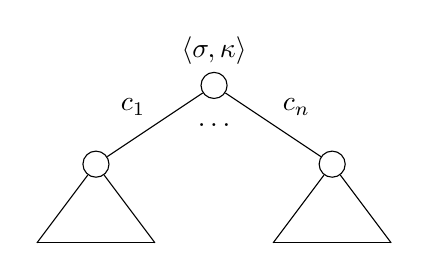
\begin{tikzpicture}[level distance = 10mm,baseline]
            \node [circle,draw] (root){}
                child {node [circle,draw] (left0){}
                    child {node (left1){}
                        edge from parent [draw=none]
                    }
                    child {node (left2){}
                        edge from parent [draw=none]
                    }
                    edge from parent node [above left] {$c_1$}
                }
                child {node [circle] {}
                    edge from parent [draw=none] node [] {$\ldots$}
                }
                child {node [circle,draw] (right0){}
                    child {node (right1){}
                        edge from parent [draw=none]
                    }
                    child {node (right2){}
                        edge from parent [draw=none]
                    }
                    edge from parent node [above right] {$c_n$}
                }
                node [left=4pt] {}
                node [above=4pt] {$\langle \sigma, \kappa \rangle$};

            \draw (left1.center) -- (left2.center);
            \draw (left0) -- (left1.center);
            \draw (left0) -- (left2.center);
            \draw (right1.center) -- (right2.center);
            \draw (right0) -- (right1.center);
            \draw (right0) -- (right2.center);
        \end{tikzpicture}
        \end{minipage}
        \caption{Before}
    \end{subfigure}\hfill%
    \begin{subfigure}[t]{.3\textwidth}
        \centering
        \begin{minipage}[t][3cm][t]{\textwidth}
        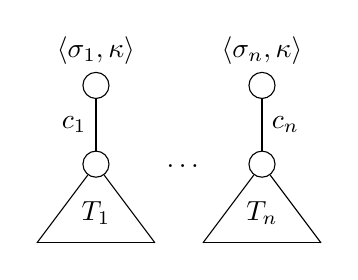
\begin{tikzpicture}[level distance = 10mm,baseline]
            \node [circle,draw] (root){}
                child {node [circle,draw] (left0){}
                    child {node (left1){}
                        edge from parent [draw=none]
                    }
                    child {node (left2){}
                        edge from parent [draw=none]
                    }
                    edge from parent node [left] {$c_1$}
                }
                node [above=4pt] {$\langle \sigma_1, \kappa \rangle$};

            \node [draw=none,below right=25pt and 22pt] {$\ldots$};

            \begin{scope}[xshift=60pt]
            \node [circle,draw] (root2){}
                child {node [circle,draw] (right0){}
                    child {node (right1){}
                        edge from parent [draw=none]
                    }
                    child {node (right2){}
                        edge from parent [draw=none]
                    }
                    edge from parent node [right] {$c_n$}
                }
                node [left=4pt] {}
                node [above=4pt] {$\langle \sigma_n, \kappa \rangle$};
            \end{scope}

            \node [below=5pt of left0] {$T_1$};
            \node [below=5pt of right0] {$T_n$};
            \draw (left1.center) -- (left2.center);
            \draw (left0) -- (left1.center);
            \draw (left0) -- (left2.center);
            \draw (right1.center) -- (right2.center);
            \draw (right0) -- (right1.center);
            \draw (right0) -- (right2.center);
        \end{tikzpicture}
        \end{minipage}
        \caption{After}
    \end{subfigure}%
    \hspace*{\fill}
    \caption{Partitioning}
    \label{fig:partition}
\end{figure}

Figure~\ref{fig:algex} illustrates how local strategies are generated from the winning abstract game tree returned by the game solver for our running example.  Figure~\ref{fig:algexa} shows $T$, the certificate tree of height 3 for the game. The algorithm starts at the root of the tree and the initial set of states and actions is given by $\sigma = s_0 \land \top = (\clk = 0 \land \curr = 0 \land \err = 0)$. The game tree defines only one winning action in the root node, hence this action is winning in all states of $\sigma$ and against all actions and no partitioning is required.  We now compute the successor set reachable by playing action $\nex = 0$ against $\sigma$: i.e. we compute the set $\sigma' \subseteq 2^{\cW'}$ such that $\exists \cS \exists \cU \exists \cC (\delta(\cS, \cU, \cC, \cS') \land \sigma \land (\nex = 0))$, which evaluates to $\sigma' = (\clk = 1 \land \err = 0)$.

\tikzset{every node/.style={solid}}
\begin{figure}[b]
    \centering
    \captionsetup[subfigure]{width=\textwidth,justification=centering}
    \begin{subfigure}[t]{.5\textwidth}
        \centering
        \begin{minipage}[t][4cm][t]{\textwidth}
        \centering
        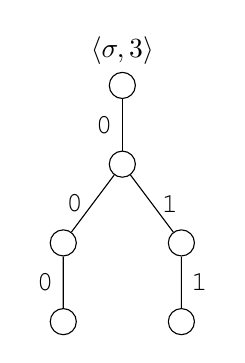
\begin{tikzpicture}[level distance = 10mm,baseline]
            \node [circle,draw] (root){}
                child {node [circle,draw] {}
                    child {node [circle,draw] {}
                        child {node [circle,draw] {}
                            edge from parent node [left] {\texttt{0}}
                        }
                        edge from parent node [left] {\texttt{0}}
                    }
                    child {node [circle,draw] {}
                        child {node [circle,draw] {}
                            edge from parent node [right] {\texttt{1}}
                        }
                        edge from parent node [right] {\texttt{1}}
                    }
                    edge from parent node [left] {\texttt{0}}
                }
                node [above=4pt] {$\langle \sigma, 3 \rangle$};
        \end{tikzpicture}
        \end{minipage}
        \caption{$T$}
        \label{fig:algexa}
    \end{subfigure}%
    \begin{subfigure}[t]{.5\textwidth}
        \centering
        \begin{minipage}[t][4cm][t]{\textwidth}
        \centering
        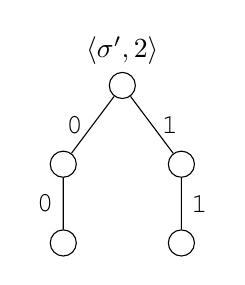
\begin{tikzpicture}[level distance = 10mm,baseline]
            \node [circle,draw] (root){}
                child {node [circle,draw] {}
                    child {node [circle,draw] {}
                        edge from parent node [left] {\texttt{0}}
                    }
                    edge from parent node [left] {\texttt{0}}
                }
                child {node [circle,draw] {}
                    child {node [circle,draw] {}
                        edge from parent node [right] {\texttt{1}}
                    }
                    edge from parent node [right] {\texttt{1}}
                }
                node [above=4pt] {$\langle \sigma', 2 \rangle$};
        \end{tikzpicture}
        \end{minipage}
        \caption{$T'$}
        \label{fig:algexb}
    \end{subfigure}
    \begin{subfigure}[t]{.5\textwidth}
        \centering
        \begin{minipage}[t][3cm][t]{\textwidth}
        \centering
        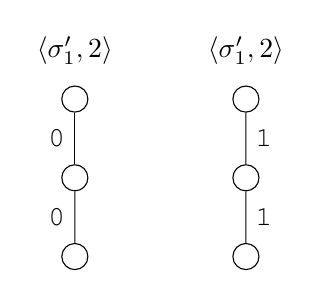
\begin{tikzpicture}[level distance = 10mm,baseline]
            \node [circle,draw] (root1){}
                child {node [circle,draw] {}
                    child {node [circle,draw] {}
                        edge from parent node [left] {\texttt{0}}
                    }
                    edge from parent node [left] {\texttt{0}}
                };
            \node [above=4pt of root1] {$\langle \sigma_1', 2 \rangle$};

            \node [circle,draw,right=2cm] (root2){}
                child {node [circle,draw] {}
                    child {node [circle,draw] {}
                        edge from parent node [right] {\texttt{1}}
                    }
                    edge from parent node [right] {\texttt{1}}
                };
            \node [above=4pt of root2] {$\langle \sigma_1', 2 \rangle$};
        \end{tikzpicture}
        \end{minipage}
        \caption{Partitioning of $T'$ into $T_1'$ and $T_2'$}
        \label{fig:algexc}
    \end{subfigure}%
    \begin{subfigure}[t]{.5\textwidth}
        \centering
        \begin{minipage}[t][3cm][t]{\textwidth}
        \centering
        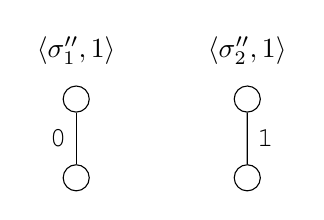
\begin{tikzpicture}[level distance = 10mm,baseline]
            \node [circle,draw] (root1){}
                child {node [circle,draw] {}
                    edge from parent node [left] {\texttt{0}}
                };
            \node [above=4pt of root1] {$\langle \sigma_1'', 1 \rangle$};

            \node [circle,draw,right=2cm] (root2){}
                child {node [circle,draw] {}
                    edge from parent node [right] {\texttt{1}}
                };
            \node [above=4pt of root2] {$\langle \sigma_2'', 1 \rangle$};
        \end{tikzpicture}
        \end{minipage}
        \caption{$T_1''$ and $T_2''$}
        \label{fig:algexd}
    \end{subfigure}
    \caption{Operation of the strategy extraction algorithm on the example}
    \label{fig:algex}
\end{figure}

Next, we descend down the tree and consider subtree $T'$ and its initial set $\sigma'$ (Figure~\ref{fig:algexb}).  We partition $\sigma'$ into subsets $\sigma_1' = (\clk = 1 \land \err = 0 \land \inp = 0)$ and $\sigma_2' = (\clk = 1 \land \err = 0 \land \inp = 1)$ that are winning for the left and right subtrees of $T'$ respectively, i.e., from $(\clk = 1 \land \err = 0)$ the controller must play action $\nex = 0$ when the environment plays $\inp = 0$, and $\nex = 1$ for $\inp = 1$.  Consider the resulting subtrees $T'_1$ and $T'_2$ with initial sets $\sigma'_1$ and $\sigma'_2$ (Figure~\ref{fig:algexc}).  We compute successor states as before: $\sigma''_1 = (\clk = 1 \land \curr = 0 \land \err = 0)$ and $\sigma''_2 = (\clk = 1 \land \curr = 1 \land \err = 0)$, with corresponding subtrees $T''_1$ and $T''_2$ (Figure~\ref{fig:algexd}).  Both subtrees have one branch; hence the actions in those branches $\nex = 0$ and $\nex = 1$ are winning for $\sigma''_1$ and $\sigma''_2$ respectively.

The algorithm returns the set of tuples $(\sigma, c, k)$.  Each tuple represents a fragment of the strategy in some tree node, where $\sigma \subseteq 2^{\cW}$ is the winning set in this node, $c \in 2^\cC$ is the controller action to play in this set, and $k$ is the distance from the node to the bottom of the tree.

Putting together fragments of the winning strategy computed above, we obtain the partial strategy shown below for this example. The compilation process must obey certain rules in order to correctly produce a winning partial strategy, the precise methodology is given below.  A complete strategy can be constructed by asigning arbitrary actions to all other states as they are known to be unreachable by playing the partial strategy.
\begin{align*}
    \pi(\clk = 0 \land \curr = 0 \land \err = 0) &= (\nex = 0) \\
    \pi(\clk = 1 \land \err = 0 \land \inp = 0) &= (\nex = 0) \\
    \pi(\clk = 1 \land \err = 0 \land \inp = 1) &= (\nex = 1) \\
    \pi(\clk = 0 \land \curr = 1 \land \err = 0) &= (\nex = 1)
\end{align*}



%%%\subsection{Local Strategies}

%%%Algorithm~\ref{alg:strat} shows the pseudocode of the strategy generation algorithm.  The algorithm proceeds in two phases: the first phase (\textsc{genLocalStrats}) computes local strategies in nodes of $T$; the second phase (\textsc{compileStrat}) compiles all local strategies into a winning strategy function.

%%%The \textsc{genLocalStrats} function recursively traverses the certificate tree $T$, starting from the root, computing local strategies in each node.  The main operation of the algorithm, called \textsc{partition}, splits $(T, s, \top)$ into $j$ tuples $(T_i, s_i, u_i)$, as shown in Figure~\ref{fig:partition}.  Each tree $T_i$ is a copy of a single branch of $T$.  The partitioning is constructed in such a way that the action $c_i$ that labels the root edge of $T_i$ is a winning controller action in $s_i$ against environment action $u_i$.

%%%Consider each tuple $(T_i, s_i, u_i)$ (lines~\ref{alg:strat:for}-\ref{alg:strat:endfor}). We descend down the tree and compute the controller strategy in the child subtree $T_i'$ of $T_i$ (right-hand side of Figure~\ref{fig:partition}).  To do so, we first compute the set of $c_i$-successors of $(s_i, u_i)$: More precisely, we compute an overapproximation $\mathcal{I} \supseteq \{ s_i' \mid \delta(s_i, u_i, c_i, s_i') \}$, such that $T_i'$ is a certificate tree for $\mathcal{I}$.  Such an overapproximation is returned by the \textsc{next} function in line~\ref{alg:strat:next}.  We can now recursively invoke the strategy generation function to compute a winning strategy for the subtree $T_i'$ from $\mathcal{I}$ (line~\ref{alg:strat:rec}).

\begin{algorithm}
   \caption{Computing a winning strategy}\label{alg:strat}
   \begin{algorithmic}[1]
        \Function{GenStrategy}{$T$, $k$, $\sigma$}
            \State $Strat \gets \Call{GenLocalStrats}{T, k, \sigma}$
            \State \Return{$\Call{CompileStrat}{Strat}$}
        \EndFunction
        \Statex

        \Function{GenLocalStrats}{$T$, $k$, $\sigma$}
            \State $[(e_1, n_1),\ldots,(e_j, n_j)] \gets \Call{succ}{T}$
            \State $[(T_1,\sigma_1),\ldots,(T_j, \sigma_j)] \gets \Call{partition}{T, k, \sigma}$
            \State $Strat \gets \{(\sigma_i, \Call{action}{e_i}, \Call{height}{k, T}) \mid i \in[1,\ldots,j]\}$\label{alg:strat:strati}
            \For{$i = 1$ to $j$}\label{alg:strat:for}
            \State $(T_i', \sigma_i') \gets \Call{next}{T_i, k, \sigma_i}$\label{alg:strat:next}
                \State $Strat_i \gets \Call{GenLocalStrats}{T_i', k-1, \sigma_i'}$\label{alg:strat:rec}
                \State $Strat \gets Strat \cup Strat_i$
            \EndFor\label{alg:strat:endfor}
            \State \Return{$Strat$} \label{alg:strat:return}
        \EndFunction
    \end{algorithmic}
\end{algorithm}


\subsection{Partitioning game trees}

The algorithm described so far involves two potentially costly operations: winning set partitioning and successor set computation.  If implemented na\"ively in a SAT based approach these operations can lead to unacceptable performance. Both operations must return sets and enumerating sets of satisfying assignments with SAT is inefficient. The key insight behind our solution is that both operations can be efficiently approximated from the proof of unsatisfiability of the formula $\sigma \land \opptf(k, T)$, with the help of interpolation, as described below.  The resulting approximations are sound, i.e., preserve the correctness of the resulting strategy.

The \textsc{partition} function (Algorithm~\ref{alg:strat:partition}) computes a local strategy in the root of an abstract game tree.  It takes a tuple $(T, k, \sigma)$, such that $T$ is a certificate tree of height $k$ for $\sigma \in 2^\cW$ and partitions $\sigma$ into subsets $\sigma_i$ such that the controller can win a game of $k$ rounds in the states and against the environment actions contained in $\sigma_i$ by choosing action $c_i$.

\begin{algorithm}[t]
   \caption{Partitioning winning states}\label{alg:strat:partition}
   \begin{algorithmic}[1]
        \Function{partition}{$T$, $k$, $\sigma$}
        \State $\hat{\sigma} \gets \sigma$
        \State $\hat{T} \gets T$
        \For{$i = 1$ to $j$}
        \State $(T_i, \tilde{T}) \gets \Call{split}{\hat{T}}$\label{alg:partition:split}
            \State $A \gets \sigma \land \Call{\opptf}{k, \tilde{T}} $ \label{alg:strat:partition:Bi}
            \State $B \gets \Call{\opptf}{k, T_i} $ \label{alg:strat:partition:Ai}
            \State $\mathcal{I} \gets \Call{interpolate}{A, B}$\label{alg:partition:I}
            \State $\sigma_i \gets \mathcal{I}(\cW_T) \land \sigma$\label{alg:partition:Ii}
            \State $\hat{\sigma} \gets \hat{\sigma} \land \neg \sigma_i$
            \State $\hat{T} \gets \tilde{T}$\label{alg:partition:upd}
        \EndFor
        \State \Return{$[(T_1, \sigma_1),\ldots, (T_j, \sigma_j)]$} \label{alg:strat:partition:return}
        \EndFunction
    \end{algorithmic}
\end{algorithm}

At every iteration, the algorithm splits the tree into the leftmost branch $T_i$ and the remaining tree (Figure~\ref{fig:split}).  It then computes $\sigma_i$ where the controller wins by following the branch $T_i$, and removes $\sigma_i$ from the current $\hat{\sigma}$.  At the next iteration it considers the leftover tree $\tilde{T}$ and state-action set $\hat{\sigma}$.

\begin{figure}
    \centering
    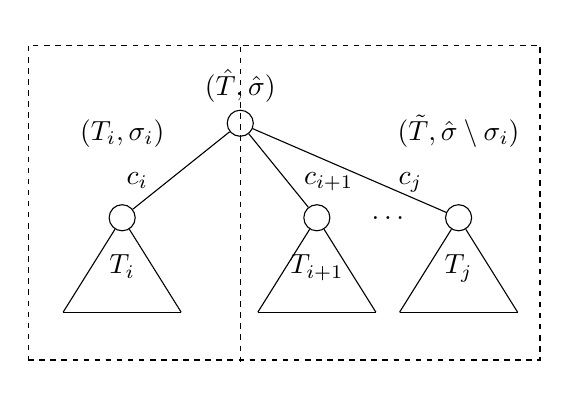
\begin{tikzpicture}[level distance = 12mm,baseline]
        \node [circle,draw] (root){}
            child {node [circle,draw] (left0){}
                child {node (left1){}
                    edge from parent [draw=none]
                }
                child {node (left2){}
                    edge from parent [draw=none]
                }
                edge from parent node [below left=-1mm and 3mm] {$c_i$}
            }
            child {node [circle,draw,right=8mm] (leftb0){}
                child {node (leftb1){}
                    edge from parent [draw=none]
                }
                child {node (leftb2){}
                    edge from parent [draw=none]
                }
                edge from parent node [below right=-1mm and 2mm] {$c_{i+1}$}
            }
            child {node [circle,draw,right=11mm] (leftc0){}
                child {node (leftc1){}
                    edge from parent [draw=none]
                }
                child {node (leftc2){}
                    edge from parent [draw=none]
                }
                edge from parent node [below right=-1mm and 5mm] {$c_{j}$}
            }
            node [above=4pt] {$(\hat{T}, \hat{\sigma})$};


        \node [draw,
            dash pattern=on 2pt off 2pt,
            minimum width=6.5cm,
            minimum height=4cm,
            below right=-10mm and -27mm
            ] {};
        \node [above=8mm of root] (startline) {};
        \node [below=29mm of root] (endline) {};
        \draw [dash pattern=on 2pt off 2pt] (startline) -- (endline);

        \node [below=5pt of left0] {$T_i$};
        \node [below=5pt of leftb0] {$T_{i+1}$};
        \node [below=5pt of leftc0] {$T_j$};
        \draw (left1.center) -- (left2.center);
        \draw (left0) -- (left1.center);
        \draw (left0) -- (left2.center);
        \draw (leftb1.center) -- (leftb2.center);
        \draw (leftb0) -- (leftb1.center);
        \draw (leftb0) -- (leftb2.center);
        \draw (leftc1.center) -- (leftc2.center);
        \draw (leftc0) -- (leftc1.center);
        \draw (leftc0) -- (leftc2.center);
        \node [right=4mm of leftb0] {$\ldots$};
        \node [above=6mm of left0] {$(T_i, \sigma_i)$};
        \node [above=6mm of leftc0] {$(\tilde{T}, \hat{\sigma} \setminus \sigma_i)$};
    \end{tikzpicture}
    \caption{Splitting of $T$ in the \textsc{Partition} function.\label{fig:split}}
\end{figure}

The algorithm maintains the invariant that $\hat{T}$ is a certificate tree of height $k$ for $\hat{\sigma}$, and hence $\hat{\sigma} \land \opptf(k, \hat{T})$ is unsatisfiable.  We decompose this formula into two conjuncts $A \land B$ such that $A$ and $B$ only share state and action variables $\cW_T$ in the root node of $T$ and that the interpolant $\mathcal{I}$ of $A$ and $B$ consists of states and environment actions for which the controller can win by following the $T_i$ subtree.  Hence $\mathcal{I}(\cW_T)$ gives us the desired set $\sigma_i$.  

Informally, $A$ is a partial expansion of the game formula induced by $\tilde{T}$.  It is satisfiable iff there exists a spoiling environment strategy from $\hat{\sigma}$ against abstract game tree $\tilde{T}$.  $B$ is a partial expansion of the game induced by $T_i$.  It is satisfiable iff there exists a spoiling environment strategy against $T_i$.  Both $A$ and $B$ can be satisfiable individually, but because $T$ is a certificate tree their conjunction is unsatisfiable.

The interpolant $\mathcal{I}$ of $A$ and $B$ implies $\neg B$, i.e., for any state and environment action in $\mathcal{I}$, $c_i$ is a winning move.  $\mathcal{I}$ is also implied by $A$, i.e., it contains all states and environment actions in $\hat{\sigma}$ for which the controller cannot win by picking moves from $\tilde{T}$ as a subset.  Equivalently, for any state and action in $\hat{\sigma} \land \neg \mathcal{I}(\cW_T)$, the controller \emph{can} win by following $\tilde{T}$, i.e., $\tilde{T}$ is a certificate tree for $\hat{\sigma} \land \neg \mathcal{I}(\cW_T)$, and we can apply the decomposition again to $\tilde{T}$ at the next iteration.


\makeatletter
\newcommand{\pushright}[1]{\ifmeasuring@#1\else\omit\hfill$\displaystyle#1$\fi\ignorespaces}
\makeatother

We prove useful properties of the $\partition$ function. We begin with the proposition that $A$ and $B$ imply a decomposition of $\hat{\sigma} \land \opptf(k, \hat{T})$. 
\begin{proposition}\label{prop:aandb}
    $A\land B \implies \hat{\sigma} \land \opptf(k, \hat{T})$.
\end{proposition}
\begin{proof}
    \begin{align*}
        A \land B ={}& (\hat{\sigma} \land \opptf(k, \tilde{T})) \land \opptf(k, T_i) \\
        A \land B ={}& \hat{\sigma} \land \bigg( E({\mathcal{S}_{\tilde{T}})} \lor \\
                     & \pushright{ \bigvee_{\langle e, n \rangle \in \textsc{succ}(\tilde{T})} \delta({\mathcal{S}_{\tilde{T}}}, {\mathcal{U}_{\tilde{T}}}, {\mathcal{C}_{\tilde{T}}}, {\mathcal{S}_n}) \land \textsc{action}(e) \land \opptf(k, n) \bigg)} \\
                     & \pushright{\land \bigg( E({\mathcal{S}_{T_i}}) \lor (\delta({\mathcal{S}_{T_i}}, {\mathcal{U}_{T_i}}, {\mathcal{C}_{T_i}}, {\mathcal{S}_{n_i}}) \land \textsc{action}(e_i) \land \opptf(k, n_i)) \bigg)} \\
        \implies{}& \hat{\sigma} \land \bigg( E({\mathcal{S}_{\hat{T}}}) \lor \\
                  & \pushright{  \bigvee_{\langle e, n \rangle \in \textsc{succ}(\hat{T})} \delta({\mathcal{S}_{\hat{T}}}, {\mathcal{U}_{\hat{T}}}, {\mathcal{C}_{\hat{T}}}, {\mathcal{S}_n}) \land \textsc{action}(e) \land \opptf(k, n) \bigg)} \\
        ={}& \hat{\sigma} \land \opptf(k, \hat{T})
    \end{align*}
\end{proof}

\begin{proposition}
    The following invariant is maintained throughout the execution of \textsc{partition}: $\hat{T}$ is a certificate tree of height $k$ for $\hat{\sigma}$.
\end{proposition}
\begin{proof}
    We prove by induction. It is a precondition of the function that $T$ is a certificate tree for $\sigma$, thus the invariant holds for the initial values $\hat{T} = T$ and $\hat{\sigma} = \sigma$.  By the induction hypothesis $(\hat{\sigma} \land \opptf(k, \hat{T}))$ is unsatisfiable, so by Proposition~\ref{prop:aandb} $(A \land B)$ must also be unsatisfiable.  Hence the interpolation operation in line~\ref{alg:partition:I} is well defined.  By the properties of interpolants, $(A \implies \mathcal{I})$, hence $(\neg \mathcal{I} \implies \neg A)$ or equivalently $(\neg\mathcal{I} \implies \neg (\hat{\sigma} \land \opptf(k, \tilde{T}))$.

    After $\hat{T}$ and $\hat{\sigma}$ are updated in line~\ref{alg:partition:upd}, their new values $\hat{T}'$ and $\hat{\sigma}'$ satisfy the following equalities: \begin{align*}
        \hat{\sigma}' \land \opptf(k, \hat{T}') ={}& \hat{\sigma} \land \opptf(k, \tilde{T}) \land \neg\mathcal{I} \\
        ={}& \neg\mathcal{I} \land \hat{\sigma} \land \opptf(k, \tilde{T}) \\
        \implies{}& \neg (\hat{\sigma} \land \opptf(k, \tilde{T})) \\
                  & \pushright{\land \hat{\sigma} \land \opptf(k, \tilde{T})} \\
        ={}& \bot
\end{align*} and hence the invariant is maintained.
\end{proof}

\begin{proposition}\label{prop:partition}
    Let $T$ be a certificate tree for $\sigma$ and let $\sigma \land \lnot E(\cS_T) = \bot$. Then $[(T_1, \sigma_1),\ldots,(T_j, \sigma_j)] = \textsc{partition}(T, k, \sigma)$ is a local winning strategy in the root of $T$, i.e., the following properties hold:
    \begin{enumerate}
        \item $\sigma_1 ,\ldots, \sigma_j$ is a partitioning of
            $\sigma$: $$\sigma = \bigvee \sigma_i \text{ and } \forall i, k. (i \neq k) \implies (\sigma_i \land \sigma_k = \bot).$$
        \item $T_i$ is a certificate tree of height $k$ for $\sigma_i$.
    \end{enumerate}
\end{proposition}
\begin{proof}
    At every iteration of the algorithm, we partition $\hat{\sigma}$ into $\sigma_i = \mathcal{I}(\cW_T) \land \hat{\sigma}$ and $\hat{\sigma} \land \neg\mathcal{I}(\cW_T)$. Hence, by construction, no $\sigma_i$ overlaps with any $\sigma_k$.

    At the final iteration of the algorithm, the tree $\tilde{T}$ consists of a single root node without outgoing branches.  Hence, $A = \hat{\sigma} \land \opptf(k, \tilde{T}) = \hat{\sigma} \land \neg E(\cS_{\tilde{T}}) = \hat{\sigma}$.  Since $(A \implies \mathcal{I})$, we get $(\hat{\sigma} \implies \mathcal{I})$ and therefore $\mathcal{I} \land \hat{\sigma} = \hat{\sigma}$, i.e., all states and actions in $\hat{\sigma}$ are included in the final set $\sigma_j$ and hence the partitioning completely covers the set $\sigma$: $\sigma=\bigvee \sigma_i$.

    We prove the second statement of the proposition.  The set $\sigma_i$ is computed as $\mathcal{I}(\cW_T) \land \hat{\sigma}$ at the $i$th iteration of the algorithm (line~\ref{alg:partition:Ii}).
    Thus, $$\sigma_i \land \opptf(k, T_i) = \mathcal{I}(\cW_T) \land \hat{\sigma} \land \opptf(k, T_i)$$ By the properties of interpolants, $$\mathcal{I} \land B = \mathcal{I}(\cW_T) \land \opptf(k, T_i) = \bot.$$  Hence $\sigma_i \land \opptf(k, T_i) = \bot$, i.e. $T_i$ is a certificate tree for $\sigma_i$.
\end{proof}

\subsection{Computing successor states}

The \textsc{next} function (Algorithm~\ref{alg:next}) takes a set $\sigma$ and its certificate tree $T$ of height $k$, such that there is exactly one outgoing edge, labelled $c$, from the root node of $T$.  $T$ has a sole child subtree $T'$ with root node $n$.  The function computes an overapproximation $\sigma'$ of the $c$-successors of $\sigma$, such that $\sigma'$ is winning for the controller and $T'$ is a certificate tree of height $k-1$ for $\sigma'$.

\begin{algorithm}
   \caption{Successor set}\label{alg:next}
   \begin{algorithmic}[1]
        \Function{next}{$T, k, \sigma$}
        \State $[(e, n)] \gets \Call{succ}{T}$ \Comment{$T$ has a single successor}
            \State $A \gets \sigma \land \delta(\cS_T, \cU_T, \cC_T, \cS_n) \land \Call{action}{e}$\label{alg:strat:partition:Ai}
            \State $B \gets \opptf(k, n) $\label{alg:strat:partition:Bi}
            \State $\mathcal{I} \gets \Call{interpolate}{A, B}$ \label{alg:strat:partition:I}
            \State \Return{$(n, \mathcal{I}(\mathcal{S}_{n}))$} \label{alg:strat:partition:return}
        \EndFunction
    \end{algorithmic}
\end{algorithm}

Once again, we decompose the unsatisfiable formula $\sigma \land \opptf(k, T)$ into two conjuncts $A$ and $B$.  $A$ encodes one round of the game from the set $\sigma$, where the controller plays action $c$.  $B = \opptf(k, T')$ is a partial $\forall$-expansion of the game induced by $T'$.  $A$ and $B$ only share state variables $\cS_n$ (where $n$ is the root node of $T'$ and single successor node of $T$) and their interpolant gives an approximation of the set of successor states.

\begin{proposition}\label{prop:next}
    Let $T$ be a certificate tree for $\sigma$ with a single outgoing edge, labelled $c$ in its root node, and let $(T',\mathcal{I})
    = \textsc{next}(T,\sigma)$.
    Then:
    \begin{enumerate}
        \item $\mathcal{I}$ is an overapproximation of the $c$-successors of $\sigma$, i.e., $\mathcal{I} \supseteq \sigma'$ where $$\sigma' = \exists \cS \exists \cU \exists \cC (\delta(\cS, \cU, \cC, \cS') \land \sigma \land c)$$
        \item $T'$ is a certificate tree of length $k-1$ for $\sigma'$
    \end{enumerate}
\end{proposition}
\begin{proof}
    The $c$-successor set $\sigma'$ of $\sigma$ is defined by $\exists \cS \exists \cU (\delta(\cS, \cU, \cC, \cS') \land \sigma \land c)$. The matrix of this formula is exactly formula $A$.  Hence the successor set is given by $\sigma' = \exists \cS \exists \cU (A)$.  Since $(A \implies \mathcal{I})$, $\sigma' \implies \exists \cS \exists \cU (\mathcal{I})$.  Since $\mathcal{I}$ is defined over state variables in the root of $T'$ only, the quantifiers can be removed: $\sigma' \implies \mathcal{I}$ or, in the relational form, $\mathcal{I} \supseteq \sigma'$.
    
    We prove the second property by the construction of the interpolant: $(\mathcal{I} \land \opptf(k, T')) = (\mathcal{I} \land B) = \bot$.
\end{proof}

The computed set is an overapproximation of the desired set of successor states but the second property of Proposition~\ref{prop:next} guarantees that we can continue the algorithm using the approximation. The interpolant contains additional states that may not be $c$-successors of $\sigma$ but we ensure that $T'$ contains a winning strategy for these states. As a result, the partial strategy potentially covers additional unreachable states but is guaranteed to be correct.

\subsection{Compiling the strategy}

Finally, we describe how local strategies computed by \textsc{genLocalStrats} are combined into a winning strategy for the game.  This requires some care, as individual partial strategies can be defined over overlapping sets of states.  We want the resulting strategy function to be deterministic; therefore for each partial strategy we only add new states not yet covered by the computed combined strategy.  Function \textsc{compileStrats} (Algorithm~\ref{alg:compile}) achieves this by keeping track of all states $W$ already added to the strategy.  For every new tuple $(w, a, k)$, it restricts the set $w$ to $\neg W$, which guarantees that no state action pair can be added to the strategy twice.  

\begin{algorithm}[t]
   \caption{Compiling the  winning strategy}\label{alg:compile}
   \begin{algorithmic}[1]
        \Function{CompileStrat}{$Strat$}
            \State $\pi \gets \bot,~~W \gets \bot$
            \State $Strat' \gets \Call{sort}{Strat}$ \Comment{Sort by descending $k$}
            \For{$(w, c, k) \in Strat'$} 
            \State $\pi \gets \pi \lor (w \land \neg W \land c)$
                \State $W \gets W \lor w$
            \EndFor
            \State \Return $\pi$
        \EndFunction
    \end{algorithmic}
\end{algorithm}

\begin{theorem}[Correctness of the algorithm]\label{th:stratCorrectness}
Let abstract game tree $T$ of height $\kappa$ be a certificate tree for the set $\sigma = s_0 \land \top$, let $\pi$ be a partial function returned by the strategy generation algorithm, $\pi=\textsc{genStrategy}(T,\sigma)$, and let $\pi'$ be an arbitrary extension of $\pi$ to a complete function.  Then $\pi'$ is a winning controller strategy for the bounded game of length $\kappa$ with initial state $s_0$.
\end{theorem}
\begin{proof}
    $\textsc{genStrategy}$ generates a strategy $\pi$ from the set of tuples $Strat$ returned by $\textsc{genLocalStrats}$. Each tuple $(w, c, k)$ in $Strat$ is generated by \textsc{partition} and, according to Proposition~\ref{prop:partition}, $c$ is a winning controller move from $w$ for a game of length $k$. By Proposition~\ref{prop:next}, all possible $c$-successors of $w$ are covered by subsequent iterations of \textsc{partition} and therefore has some tuple $(w', c', k-1)$ in $Strat$. By constructing $\pi = \textsc{genStrategy}$ from $Strat$ in the order of highest $k$ to lowest, we ensure that any mapping defined by $\pi$ for $w'$ is from a tuple with height $\geq k-1$ and so has a strategy that is winning for the controller for a game of $k-1$ rounds or more.  
    
    Therefore $\pi$ defines a controller action for every state reachable from $s_0$ by playing the strategy. Any extension of $\pi$ to a complete function that maps unreachable states to an arbitrary controller action must then be a winning strategy since the controller is guaranteed to stay within the safe region $W$ by playing $\pi$.
\end{proof}

\section{Optimisations}

\subsection{Strategy extraction with learning}

In Section~\ref{sec:boundedLearning} I described an optimisation to bounded realisability in which computational learning is used to exclude known losing states from the search tree. If this optimisation is enabled then the final certificate tree returned by the realisability algorithm will assume that these states are winning. In this case we need to adjust the way that strategy extraction is done so that the generated strategy includes winning actions for excluded states. 

The modification is simple: partial strategies are extracted online during the realisability check. Recall that a set of states $b$ is learned to be losing for the environment for height $k$ when $b \land \opptf(k, T)$ is unsatisfiable for some subtree $T$. In other words, $T$ is a certificate tree for $b$. Algorithm~\ref{alg:stratLearning} shows \textsc{learn} with an additional call to \textsc{genLocalStrats} in line~\ref{line:onlineLocalStrats}.  We use \textsc{genLocalStrats} to record a set of partial strategies, $Strats$, one for each learned state. On termination of the bounded realisability algorithm the entire set $Strats$ is combined into a winning partial strategy with \textsc{compileStrat}.

\begin{algorithm}
    \caption{Learning with online strategy extraction}
    \label{alg:stratLearning}
    \begin{algorithmic}
        \Function{learn}{$p, s, k, T, f$}
            \State $ \hat{s} \gets s$
            \For{$s \in \cS$}
            \State $sol \gets \Call{SATWithAssumptions}{\hat{s} \setminus \{ s \}, f}$
                \If{$sol = \texttt{NULL}$}
                    \State $\hat{s} \gets \hat{s} \setminus \{ s \}$
                \EndIf
            \EndFor
            \If{$p = \texttt{cont}$}
                \State $B^c \gets B^c \lor \hat{s}$
            \Else
                \State $Strats \gets Strats \cup \Call{genLocalStrats}{T, k, \hat{s} \land \top}$ \label{line:onlineLocalStrats}
                \For{$i \in [0,\ldots,k]$}
                    \State $B^e[i] \gets B^e[i] \lor \hat{s}$
                \EndFor
            \EndIf
        \EndFunction
    \end{algorithmic}
\end{algorithm}

Algorithm~\ref{alg:stratTreeFml} (reproduced from the previous chapter) shows how an opponent tree formula is constructed with respect to an indexed array of sets of learned states $B^e$. At each index $k$ of the array is a set of states for which the environment is known to lose a game of $k$ rounds. $B^e$ conceptually consists of pairs of state sets and tree heights $(b_i, k_i)$ for which $\textsc{findCandidate}(\textsc{env}, b_i, k_i, T_i)$ returned false for some abstract game tree $T_i$, i.e. $T_i$ is a certificate tree for $(b_i, k_i)$.

\begin{algorithm}
    \caption{Opponent tree formula with state learning}
    \label{alg:stratTreeFml}
    \begin{algorithmic}[1]
        \Function{\textoverline{treeFormula}}{$k, T$}
        \If{$\Call{height}{k, T} = 0$}
        \State \Return{\Call{E}{$\cS_{T}$}}
        \Else
        \State \Return{\Call{$B^e$[\Call{height}{$k,t$}]}{$\cS_{T}$} $\lor$ \\
        $$\bigvee_{\langle e, n \rangle \in \Call{succ}{T}}(\Call{$\delta$}{\cS_T, \cU_T, \cC_e, \cS_n} \land \cC_e = \Call{action}{e} \land \Call{\textoverline{treeFormula}}{k, n})$$ }
        \EndIf
        \EndFunction
    \end{algorithmic}
\end{algorithm}

\begin{theorem}
    Let $G$ be a bounded safety game that is realisable with respect to an error set $E$ and a bound $k$. Let $Strats$ be a set of partial strategies generated during $\textsc{solveAbstract}$, then $\pi = \textsc{compileStrat}(Strats)$ is a winning partial controller strategy for $G$.
\end{theorem}
\begin{proof}
    We prove correctness inductively. At the first online call to \textsc{genLocalStrats}, $B^e$ is empty and by Theorem~\ref{th:stratCorrectness} $Strat_0$ is a partial strategy for a state-round pair $(b_0, k_0)$. $Strat_0$ is added to $Strats$.
    
    In subsequent calls all interpolants are constructed such that $B^e$ is excluded from the game. So, $Strat_{j+1}$ is a partial strategy for a game beginning at $b_{j+1}$ and of length $k_{j+1}$ where every state-round pair $(b_0, k_0), \ldots, (b_k, k_j)$ is assumed unreachable. As in Theorem~\ref{th:stratCorrectness}, all tuples $(w, c, k)$ in $Strat_{j+1}$ are such that $c$ is a winning controller action from $w$ for a game of length $k$ if all $(b_0, k_0), \ldots, (b_k, k_j)$ is assumed unreachable. Likewise, every $c$-successor of $w$ is either covered by $Strat_{j+1}$ or is contained in $(b_0, k_0), \ldots, (b_k, k_j)$.

    Under the inductive hypothesis, $Strats = Strat_0 \cup \ldots \cup Strat_j$ contains winning partial strategies for every $(b_0, k_0), \ldots, (b_j, k_j)$. Thus every state assumed unreachable at the $j+1$ iteration has a winning partial strategy in $Strat_0 \cup \ldots \cup Strat_j$ and so $Strat_0 \cup \ldots \cup Strat_{j+1}$ contains winning partial strategies for all $(b_0, k_0), \ldots, (b_{j+1}, k_{j+1})$.

    Thus, $Strats$ contains winning partial strategies for every state in $B^e$.  \textsc{solveAbstract} terminates when it discovers a certificate tree for the initial state $s_0$. As with all certificate trees generated during execution the algorithm learns from the tree via a call to \textsc{learn}. Thus, at termination $s_0 \in B^e[k]$ and $Strats$ contains a winning partial strategy from $s_0$. Therefore $\pi = \textsc{compileStrat}(Strats)$ is a winning partial controller strategy for the game.
\end{proof}

\subsection{Ensuring compact interpolants}

The implementation of strategy extraction (described in further detail in Chapter~\ref{ch:evaluation}) also contains an optimisation that ensures that the size of the formulas used in the algorithm do not grow too large. Strategy extraction generates many CNF formulas that are used to construct interpolants. Those formulas also contain interpolants themselves, which are arbitrary formulas that must first be converted to CNF. The usual Tseitin transformation converts a formula to CNF by introducing variables and potentially increases the time taken to determine (un)satisfiability and construct a new interpolant.  We optimise the implementation by constructing a BDD from each interpolant and using the BDD to efficiently enumerate cubes. A set of cubes usually requires fewer additional variables than an arbitrary circuit to represent in CNF.

BDD sweeping is used to reduce the size of formulas by carefully constructing BDDs from subformulas to deduplicate equivalent parts of the formula~\cite{Kuehlmann97}. The sweep is done carefully so that no one BDD grows too large. For this optimisation a complete BDD sweeping implementation was not required since in practice the BDDs constructed from these interpolants never grew too large. However, if a problem instance was found to generate interpolants that are difficult to represent then BDD sweeping could be used here.

\section{Related work}

All existing strategy extraction algorithms for games were developed for use with game solvers based on winning set compilation~\cite{Bloem14}.  Such a solver generates a sequence of expanding state sets for which the game is safe for $1,2,\ldots$ steps.  The task of the strategy extraction algorithm is to compute a function that in every winning state chooses a single move that forces the game back into a safe state.  In contrast, our strategy generation algorithm does not require the game solver to compile winning regions, but instead uses abstract game trees.

Another line of related work is strategy extraction algorithms for QBF used in QBF certification. QBF strategy extraction methods are specific to the underlying proof system used by the QBF search algorithm~\cite{Lonsing10,Egly13,Goultiaeva11}.  A strategy in a QBF is an oracle that, given the history of moves played in the game, outputs the next move for the winning player.  An additional procedure is required to convert this oracle into a memory-free strategy function that maps a state to a controller move.  Our work can been seen as such a procedure for $\forall Exp+Res$ proof system based solvers~\cite{Janota13}.

\section{Summary}

%%%I have presented a strategy extraction algorithm to extended bounded realisability to bounded synthesis. The algorithm assigns controller actions to pairs of states and environment actions by a lightweight recursive application of interpolation to the certificate tree generated by the game solver. The performance overhead of this approach will be evaluated in Chapter~\ref{ch:evaluation}.

I have presented a strategy extraction algorithm to extend bounded realisability to bounded synthesis. The performance overhead of this approach will be evaluated in Chapter~\ref{ch:evaluation}.

\begin{itemize}
    \item A strategy may be extracted from the certificate tree generated by the bounded realisability algorithm. The winning controller actions are given in the edges of the certificate tree and the algorithm must simply assign actions to subsets of the combined state and environment action space.

    \item A set of states and environment actions may be partitioned such that a controller action is winning for each partition. This can be approximated efficiently using Craig interpolation.  Likewise, for a set of state and environment actions the successor states with respect to a controller action may be approximated by an interpolant. These two operations implemented by efficient approximations are sufficient to construct a strategy from a certificate tree.

    \item The algorithm may also be used, with some modification, to extract a spoiling strategy for the environment. Another modification enables compatibility with the computational learning optimisation of bounded realisability.

\end{itemize}


\chapter{Unbounded Realisability}
\label{ch:unbounded}

\newtheorem*{exmpInt}{Example: Why we use interpolants}

In previous chapters I outlined an algorithm to solve bounded realisability games and an extension that can extract strategies from the result. Bounded realisability can be used to prove the existence of a winning strategy for the environment on the unbounded game by providing a witness. For the controller, the strongest claim that can be made is that the strategy is winning as long as the game does not extend beyond the maximum bound. The work described in this chapter can be used to address this by presenting another extension to the algorithm that solves unbounded realisability games.

The baseline solution to this problem is to set a maximum bound such that all runs in the unbounded game will be considered. The na\"ive approach is to use size of the state space as the bound ($2^\mathcal{S}$) so that all states may be explored by the algorithm. A more nuanced approach is to use the diameter of the game \cite{Biere99}, which is the smallest number $d$ such that for any state $x$ there is a path of length $\leq d$ to all other reachable states. Computing the diameter, however, is also expensive and solving a game bounded to the size of the diameter may be infeasible.

Instead I present an approach that iteratively solves games of increasing
bound while learning bad states from abstract games using Craig interpolation. We utilise the approximation properties of the interpolant to construct sets of states that underapproximate the total losing set for the controller. By underapproximating we avoid constructing a potentially large representation of this set that could be the cause of infeasibility in a BDD solver. Later in this chapter we will see that a careful construction of approximate sets enables a fixed point that is sufficient to prove the nonexistence of an environment-winning strategy.

\section{Algorithm}
\label{sec:unboundedAlgorithm}

Recall the bounded realisability algorithm from Chapter~\ref{ch:bounded}. A safety game is solved with respect to a bound on the number of game rounds. The algorithm is a counterexample guided approach that constructs abstractions of the game in the form of game trees. An abstract game tree restricts one player to the actions that label edges in the tree. In Chapter~\ref{ch:strategy} I presented a strategy extraction procedure that utilises the abstract game tree as a certificate for the game. In this chapter I introduce a similar approach that extracts an approximation of winning states from the certificate tree.

The bounded algorithm is reproduced in Algorithm~\ref{alg:unboundedBounded} with some modifications. The algorithm solves a game $(\mathcal{S}, \mathcal{U}, \mathcal{C}, \delta, s_0)$ with state variables $\mathcal{S}$, environment variables $\mathcal{U}$, controller variables $\mathcal{C}$, transition relation $\delta$, and initial states $s_0$. The safety condition of the game is defined by a set of error states $E$ that the controller must avoid and the environment must reach. The unbounded algorithm is modified to learn states when a candidate cannot be found for an abstract game (line~\ref{alg:unboundedBounded:learn}).

\begin{algorithm}
    \begin{algorithmic}[1]
        \Function{solveAbstract}{$p, s, k, T$}
        \State $cand \gets $ \Call{findCandidate}{$p, s, k, T$} 
        \IIf{$k = 1$} \Return $cand$ \EndIIf 
        \State $T' \gets T$
        \Loop
            \IIf{$cand = \texttt{NULL}$} \Return $\texttt{NULL}$ \EndIIf 
            \State $\langle cex, l, u \rangle \gets $ \Call{verify}{$p, s, k, T, cand$} 
            \IIf{$cex = \False$} \Return $cand$ \EndIIf 
            \State $T' \gets $ \Call{append}{$T', l, u$} 
            \State $cand \gets $ \Call{solveAbstract}{$p, s, k, T'$} 
        \EndLoop
        \EndFunction
        \algstore{b1}
    \end{algorithmic}

    \begin{algorithmic}
        \algrestore{b1}
        \Function{findCandidate}{$p, s, k, T$}
        \State $\hat{T} \gets $ \Call{extend}{$T$}
            \State $f \gets $ \IfElse{$p = \texttt{cont}$}{\Call{treeFormula}{$k, \hat{T}$}}{\Call{\textoverline{treeFormula}}{$k, \hat{T}$}} \EndIfElse
            \State $sol \gets $ \Call{SAT}{$s(\mathcal{S}_{\hat{T}}) \land f$}
            \If{$sol = \texttt{unsat}$} 
                \LineComment{Unbounded solver learns states here}
                \State \IfElse{$p = \texttt{cont}$}{\Call{learn}{$s, \hat{T}$}}{\Call{\textoverline{learn}}{$s, \hat{T}$}}\label{alg:unboundedBounded:learn} \EndIfElse
                \State \Return $\texttt{NULL}$
            \Else
                \State \Return $\{ \langle n, c \rangle | n \in $ \Call{nodes}{$T$} $, c = \Call{sol}{n} \}$
            \EndIf
        \EndFunction
        \algstore{b2}
    \end{algorithmic}

    \begin{algorithmic}
        \algrestore{b2}
        \Function{verify}{$p, s, k, T, cand$}
            \For{$l \in leaves(gt)$}
            \State $\langle k', s'\rangle \gets $ \Call{outcome}{$s, k, cand, l$}
            \If{$p = \textsc{cont}$}
                \State $T' \gets \emptyset$
            \Else
                \State $T' \gets \{ cand(l) \}$
            \EndIf
                \State $a \gets $ \Call{solveAbstract}{\Call{opponent}{$p$}, $s'$, $k'$, $T'$}
                \IIf{$a \neq \texttt{NULL}$} \Return $\langle \True, l, a \rangle$ \EndIIf
            \EndFor
            \State \Return $\langle \False, \emptyset, \emptyset \rangle$
        \EndFunction
    \end{algorithmic}

    \caption{Unbounded realisability}
    \label{alg:unboundedBounded}
\end{algorithm}

%%%The states in an abstract game with no controller candidate are
%%%\emph{must-losing}. The environment can always force the game into the error
%%%states from these states.

%%%From abstractions with no environment candidate we record the complement of
%%%states in the tree as \emph{may-losing}. The environment cannot reach the error
%%%state in a number of steps equal to the distance to the bottom of the tree.

%%%We maintain a set of states for each rank up to the current bound. We maintain
%%%an invariant over these sets via careful construction so that they are
%%%monotonically increasing by rank. We also ensure that the environment is unable
%%%to force play from one set to the next. Due to these invariants, when two
%%%adjacent sets become equivalent we know that the algorithm has reached a fixed
%%%point and the controller is winning in the unbounded game (line 6).

We extend the bounded synthesis algorithm to learn states losing for one of the players from failed attempts to find candidate strategies.  The learning procedure kicks in whenever \textsc{findCandidate} cannot find a candidate strategy for an abstract game tree. We can learn additional losing states from the tree via interpolation.  This is achieved in line~\ref{alg:unboundedBounded:learn} in Algorithm~\ref{alg:unboundedBounded}, enabled in the unbounded version of the algorithm, which invokes \textsc{learn} or \textsc{\textoverline{learn}} to learn controller or environment losing states respectively (Algorithm~\ref{alg:learn}).  

%%%For the controller, this means the environment partial strategy represented by $T$
%%%will always reach $E$ from $s$ no matter the assignments to $C$ variables (the
%%%bound is irrelevant).  For the environment, the controller can avoid $E$ for $k$
%%%rounds no matter the assignments to $U$ variables. Hence, we have established
%%%that $s$ is a losing state either always (for the controller) or for bound $k$
%%%(for the environment). 



\subsection{Example}

Consider a simple arbiter system in which the environment makes a request for a number of resources (1 or 2), and the controller may grant access to up to two resources.  The total number of requests grows each round by the number of environment requests and shrinks by the number of resources granted by the controller in the previous round.  The controller must ensure that the number of unhandled requests does not accumulate to more than 2.  Figure~\ref{fig:example} shows the variables (\ref{fig:examplevars}), the initial state of the system (\ref{fig:exampleinit}), and the formulas for computing next-state variable assignments (\ref{fig:exampletrans}) for this example. We use primed identifiers to denote next-state variables and curly braces to define the domain of a variable.


\begin{figure}
    \begin{subfigure}[t]{\textwidth}
        \centering
        \begin{tabular}{l | l | l}
            \textbf{Uncontrollable} & \textbf{Controllable} & \textbf{State} \\
            \hline
            \texttt{request = \{1,2\}} & \texttt{grant0 = \{0,1\}} & \texttt{resource0 = \{0,1\}} \\
            & \texttt{grant1 = \{0,1\}} & \texttt{resource1 = \{0,1\}} \\
            & & \texttt{nrequests = \{0,1,2,3\}} \\
        \end{tabular}
        \caption{Variables}
        \label{fig:examplevars}
    \end{subfigure}

    \vspace{5mm}
    \begin{subfigure}[t]{\textwidth}
        \centering
        \texttt{resource0 = 0; resource1 = 0; nrequests = 0;}
        \caption{Initial State}
        \label{fig:exampleinit}
    \end{subfigure}

    \begin{subfigure}[t]{\textwidth}
        \begin {align*}
            \texttt{resource0'} & \texttt{ = grant0;} \\
            \texttt{resource1'} & \texttt{ = grant1;} \\
            \texttt{nrequests'} & \texttt{ = (nrequests + request >= resource0 + resource1)} \\ 
                                & \texttt{ ? (nrequests + request - resource0 - resource1)}\\
                                & \texttt{ : 0;}
        \end{align*}
        \caption{Transition Relation}
        \label{fig:exampletrans}
    \end{subfigure}
    \caption{Example}
    \label{fig:example}
\end{figure}


\begin{figure}[t]
    \centering
    \begin{subfigure}[t]{.32\textwidth}
        \centering

        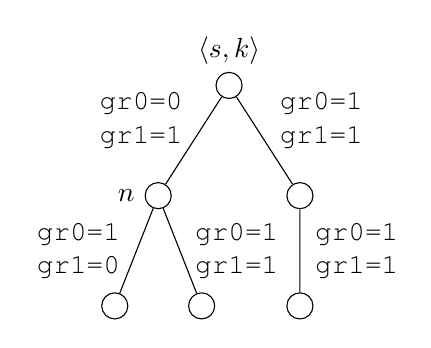
\begin{tikzpicture}[sibling distance = 18mm, level distance = 14mm]
            \node [circle,draw] (root){}
                child {node [circle,draw] {}
                    child {node [circle,draw,right=5pt] {}
                        edge from parent node [left=4pt,text width=1cm] {\texttt{gr0=1 gr1=0}}
                    }
                    child {node [circle,draw,left=5pt] {}
                        edge from parent node [right=2pt,text width=1cm] {\texttt{gr0=1 gr1=1}}
                    }
                    node [left=5pt] {$n$}
                    edge from parent node [above left=-6pt and 2pt,text width=1cm] {\texttt{gr0=0 gr1=1}}
                }
                child {node [circle,draw] (n) {}
                    child {node [circle,draw] {}
                        edge from parent node [right=2pt,text width=1cm] {\texttt{gr0=1 gr1=1}}
                    }
                    edge from parent node [above right=-6pt and 2pt,text width=1cm] {\texttt{gr0=1 gr1=1}}
                }
                node [above=4pt] {$\langle s, k \rangle$};
        \end{tikzpicture}
        \caption{A losing AGT $T$}
        \label{fig:interpolatetree}
    \end{subfigure}

    \begin{subfigure}[t]{.5\textwidth}
        \centering
        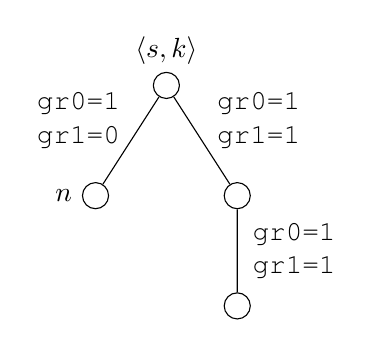
\begin{tikzpicture}[sibling distance = 18mm, level distance = 14mm]
            \node [circle,draw] (root){}
                child {node [circle,draw] {}
                    node [left=5pt] {$n$}
                    edge from parent node [above left=-6pt and 2pt,text width=1cm] {\texttt{gr0=1 gr1=0}}
                }
                child {node [circle,draw] (n) {}
                    child {node [circle,draw] {}
                        edge from parent node [right=2pt,text width=1cm] {\texttt{gr0=1 gr1=1}}
                    }
                    edge from parent node [above right=-6pt and 2pt,text width=1cm] {\texttt{gr0=1 gr1=1}}
                }
                node [above=4pt] {$\langle s, k \rangle$};
        \end{tikzpicture}
        \caption{Tree slice $T_1$}
        \label{fig:treef1}
    \end{subfigure}%
    \begin{subfigure}[t]{.5\textwidth}
        \centering
        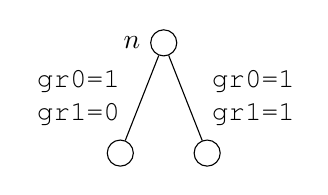
\begin{tikzpicture}[sibling distance = 18mm, level distance = 14mm]
            \node [circle,draw] {}
                child {node [circle,draw,right=5pt] {}
                    edge from parent node [left=6pt,text width=1cm] {\texttt{gr0=1 gr1=0}}
                }
                child {node [circle,draw,left=5pt] {}
                    edge from parent node [right=6pt,text width=1cm] {\texttt{gr0=1 gr1=1}}
                }
                node [left=5pt] {$n$};
        \end{tikzpicture}
        \caption{Tree slice $T_2$}
        \label{fig:treef2}
    \end{subfigure}
    \caption{Splitting of an abstract game tree by the learning procedure.}
    \label{fig:interpolanttrees}
\end{figure}

\begin{algorithm}[t]
    \begin{algorithmic}[1]
        \Require $s(\mathcal{S}_T) \land $ \Call{treeFormula}{$k, T$} $\equiv \bot$
        \Require \emph{Must-invariant} holds
        \Ensure \emph{Must-invariant} holds
        \Ensure $s(\mathcal{S}_T) \land B^M \not\equiv \bot$
        \Comment $s$ will be added to $B^M$
        \Function{learn}{$s, T$}
            \IIf{\Call{succ}{$T$} $= \emptyset$}
                \Return
            \EndIIf
            \State $n \gets $ non-leaf node with min height 
            \State $\langle T_1, T_2 \rangle \gets $ \Call{gtSplit}{$T, n$}
            \State $F_1 \gets s(\mathcal{S}_T) \land \Call{treeFormula}{k, T_1}$
            \State $F_2 \gets \Call{treeFormula}{k, T_2}$
            \State $\mathcal{I} \gets  \Call{interpolate}{F_1, F_2}$
            \State $B^M \gets B^M \lor \mathcal{I}$
            \State \Call{learn}{$s, T_1$}
        \EndFunction
        \algstore{learn}
    \end{algorithmic}
    
    \begin{algorithmic}[1]
        \algrestore{learn}
        \Require $s(\mathcal{S}_T) \land $ \Call{\textoverline{treeFormula}}{$k, T$} $\equiv \bot$
        \Require \emph{May-invariant} holds
        \Ensure \emph{May-invariant} holds
        \Ensure $s(\mathcal{S}_T) \land B^m[$\Call{height}{$k, T$}$] \equiv \bot$
        \Comment{$s$ will be removed from $B^m$}
        \Function{\textoverline{learn}}{$s, T$}
            \IIf{\Call{succ}{$T$} $= \emptyset$}
                \Return
            \EndIIf
            \State $n \gets $ non-leaf node with min height 
            \State $\langle T_1, T_2 \rangle \gets $ \Call{gtSplit}{$T, n$}
            \State $F_1 \gets s(\mathcal{S}_T) \land $ \Call{\textoverline{treeFormula}}{$k, T_1$}
            \State $F_2 \gets \Call{\textoverline{treeFormula}}{k, T_2}$
            \State $\mathcal{I} \gets $ \Call{interpolate}{$F_1, F_2$}
            \For{$i = 1$ to \Call{height}{$k, n$}}
                \State $B^m[i] \gets B^m[i] \setminus \mathcal{I}$
            \EndFor
            \State \Call{\textoverline{learn}}{$s, T_1$}
        \EndFunction
    \end{algorithmic}
    \caption{Learning algorithms}
    \label{alg:learn}
\end{algorithm}


This example is the $n=2$ instance of the more general problem of an arbiter of $n$ resources. For large values of $n$, the set of winning states has no compact representation, which makes the problem hard for BDD solvers. One approach is to compute the uncontrollable predecessor of the set of error states, i.e. the states from which the environment can force the game into an error state. In the example, one iteration of this operation would give the set: $\texttt{nrequests} = 3 \lor (\texttt{nrequests} = 2 \land ( \texttt{resource0} = 0 \lor \texttt{resource1} = 0)) \lor (\texttt{nrequests} = 1 \land (\texttt{resource0} = 0 \land \texttt{resource1} = 0))$. We try to avoid computing the entire winning set by employing interpolation to approximate it instead. The benefit of interpolation is that an approximation can be obtained efficiently from the resolution proof of two mutually unsatisfiability formulas.

Consider node $n$ in Figure~\ref{fig:interpolatetree}, which shows an abstract game tree for which the environment has no winning action. At this node there are two controller actions that prevent the environment from forcing the game into an error state in one game round. We want to use this tree to learn the states from which the controller can win playing one of these actions.

Given two formulas $F_1$ and $F_2$ such that $F_1 \land F_2$ is unsatisfiable, it is possible to construct a Craig interpolant $\mathcal{I}$ such that $F_1 \to \mathcal{I}$, $F_2 \land \mathcal{I}$ is unsatisfiable, and $\mathcal{I}$ refers only to the intersection of variables in $F_1$ and $F_2$. 

We choose a non-leaf node $n$ of $T$ with maximal depth, i.e., a node whose children are leafs (Algorithm~\ref{alg:learn}, line~3). We then split the tree at $n$ such that both slices $T_1$ and $T_2$ contain a copy of $n$ (line~4).  Figure~\ref{fig:treef1} shows $T_1$, which contains all of $T$ except $n$'s children, and $T_2$ (Figure~\ref{fig:treef2}), which contains only $n$ and its children.  There is no candidate strategy for $T$ so $s \land \textsc{\textoverline{treeFormula}}(k, T)$ is unsatisfiable.  By construction, $ (\textsc{\textoverline{treeFormula}}(k, T_1) \land \textsc{\textoverline{treeFormula}}(k, T_2)) \implies \textsc{\textoverline{treeFormula}}(k, T)$ and so we know that $(s \land$ $\textsc{\textoverline{treeFormula}}(k, T_1) \land \textsc{\textoverline{treeFormula}}(k, T_2))$ is also unsatisfiable.  

%%%This enables the construction of an interpolant that captures losing states at
%%%node $n$.

We construct an interpolant with $F_1 = s(\mathcal{S}_T) \land \textsc{treeFormula}(k, T_1)$ and $F_2 = \textsc{treeFormula}(k, T_2)$ (line~5). The only variables shared between $F_1$ and $F_2$ are the state variable copies belonging to node $n$. By the properties of the interpolant, $F_2 \land \mathcal{I}$ is unsatisfiable, therefore all states in $\mathcal{I}$ are losing against abstract game tree $T_2$ in Figure~\ref{fig:treef2}.  We also know that $F_1 \to \mathcal{I}$, thus $\mathcal{I}$ contains all states reachable at $n$ by following $T_1$ and avoiding error states.  


At node $n$, the interpolant $(\texttt{nrequests} = 1 \land
\texttt{resource1} = 1)$ captures the information we need. Any action by the
environment followed by one of the controller actions at $n$ will be
winning for the controller.

We have discovered a set $\mathcal{I}$ of states losing for the environment.
Environment-losing states are only losing for a particular bound: given that
there does not exist an environment strategy that forces the game into an error
state in $k$ rounds or less; there may still exist a longer environment-winning
strategy.  We therefore record learned environment-losing states along with
associated bounds.  To this end, we maintain a conceptually infinite array of
sets $B^m[k]$ that are may-losing for the controller, indexed by bound $k$.
$B^m[k]$ are initialised to $E$ for all $k$.  Whenever an environment-losing
set $\mathcal{I}$ is discovered for a node $n$ with bound $\textsc{height}(k,
n)$ in line~13 of Algorithm~\ref{alg:learn}, this set is subtracted from
$B^m[i]$, for all $i$ less than or equal to the bound (lines~14--16).

The \textsc{\textoverline{treeFormula}} function is modified for the unbounded
solver (Algorithm~\ref{alg:unboundedTreeFormula}) to constrain the environment
to the appropriate $B^m$. This enables further interpolants to be constructed
by the learning procedure recursively splitting more nodes from $T_1$
(Algorithm~\ref{alg:learn}, line~7) since the states that are losing to $T_2$
are no longer contained in $B^m$.

\begin{algorithm}[t] \caption{Amended tree formulas for Controller and
    Environment} \label{alg:unboundedTreeFormula} \begin{algorithmic}[1]
        \Function{treeFormula}{$k, T$} \If{$\Call{height}{k, T} = 0$} \State
        \Return{ $\lnot \Call{$B^M$}{\mathcal{S}_{T}}$ } \Else \State \Return{$\lnot
            \Call{$B^M$}{\mathcal{S}_{T}} \land$ \\ $$\bigwedge_{\langle e, n \rangle \in
            \Call{succ}{T}}(\Call{$\delta$}{\mathcal{S}_T, U_e, C_n, \mathcal{S}_n} \land U_e =
            \Call{action}{e} \land \Call{treeFormula}{k, n})$$ } \EndIf
        \EndFunction \algstore{tf1} \end{algorithmic}

    \begin{algorithmic}[1]
        \algrestore{tf1}
        \Function{\textoverline{treeFormula}}{$k, T$}
        \If{$\Call{height}{k, T} = 0$}
        \State \Return{\Call{E}{$\mathcal{S}_T$}}
        \Else
        \State \Return{ \Call{$B^m[\Call{height}{k, T}]$}{$\mathcal{S}_{T}$} $\land$ \\
            $$\bigg( \Call{E}{\mathcal{S}_T} \lor \bigvee_{\langle e, n \rangle \in \Call{succ}{T}}(\Call{$\delta$}{\mathcal{S}_T, U_n, C_e, \mathcal{S}_n} \land C_e = \Call{action}{e} \land \Call{\textoverline{treeFormula}}{k, n})\bigg)$$ }
        \EndIf
        \EndFunction
    \end{algorithmic}
\end{algorithm}

Learning of states losing for the controller is similar (\textsc{learn} in Algorithm~\ref{alg:learn}). The main difference is that environment-losing states are losing for all bounds. Therefore we record these states in a single set $B^M$ of must-losing states (Algorithm~\ref{alg:learn}, line~6).  This set is initialised to the error set $E$ and grows as new losing states are discovered.  The modified \textsc{\textoverline{treeFormula}} function (Algorithm~\ref{alg:unboundedTreeFormula}) blocks must-losing states, which also allows for recursive learning over the entire tree.

\subsection{Main synthesis loop}

Figure~\ref{alg:unbounded} shows the main loop of the unbounded synthesis algorithm.
The algorithm invokes the modified bounded synthesis procedure with increasing bound $k$
until the initial state is in $B^M$ (environment wins) or $B^m$ reaches a fixed point 
(controller wins). We prove correctness in the next section.

\begin{algorithm}[h]
    \begin{algorithmic}[1]
        \Function{solveUnbounded}{$T$}
            \State $B^M \gets E$
            \State $B^m[0] \gets E$
            \For{$k = 1 \dots$}
                \If{\Call{SAT}{$s_0 \land B^M$}}
                    \LineComment{Losing in the initial state}
                    \State \Return \texttt{unrealisable} 
                \EndIf
                \If{$\exists i < k . \  B^m[i] \equiv B^m[i+1]$}
                    \LineComment{Reached fixed point}
                    \State \Return \texttt{realisable} 
                \EndIf
                \State $B^m[k] \gets E$
                \State \Call{checkBound}{$k$}
            \EndFor
        \EndFunction
        \algstore{u1}
    \end{algorithmic}

    \begin{algorithmic}
        \algrestore{u1}
        \Require \emph{May} and \emph{must} invariants hold
        \Ensure \emph{May} and \emph{must} invariants hold
        \Ensure $s_0 \not\in B^m[k]$ if there exists a winning controller strategy with bound $k$
        \Ensure $s_0 \in B^M$ if there exists a winning environment strategy with bound $k$
%%%        $\exists u_{k..1} \forall c_{k..1} \  s(x_k) \land (E_k \lor (\delta(x_k, u_k, c_k) \land E(x_{k-1}) \lor ... \land E(x_1) \lor (\delta(x_1, u_1, c_1) \land E(x_0))...)$
%%%            $\forall u_{k..1} \exists c_{k..1} \  s(x_k) \land \lnot E_k \land \delta(x_k, u_k, c_k) \land \lnot E(x_{k-1}) \land ... \land \delta(x_1, u_1, c_1) \land \lnot E(x_0)$
        \Function{checkBound}{$k$}
            \State \Return \Call{solveAbstract}{$\texttt{env}, s_0, k, \emptyset$}
        \EndFunction
    \end{algorithmic}
    \caption{Unbounded Synthesis}
    \label{alg:unbounded}
\end{algorithm}



\section{Correctness}


We define two global invariants of the algorithm.  The \emph{may-invariant}
states that sets $B^m[i]$ grow monotonically with $i$ and that each $B^m[i+1]$
overapproximates the states from which the environment can force the game into
$B^m[i]$. We call this operation $Upre$, the uncontrollable predecessor. So the
\emph{may-invariant} is: $$\forall i<k.~B^m[i] \subseteq B^m[i+1], Upre(B^m[i])
\subseteq B^m[i+1].$$

The \emph{must-invariant} guarantees that the must-losing set $B^M$ is an
underapproximation of the actual losing set $B$: $$B^M \subseteq B.$$

Correctness of $\textsc{solveUnbounded}$ follows from these invariants. The
must-invariant guarantees that the environment can force the game into an error
state from $B^M$, therefore checking whether the initial state is in $B^M$ (as
in line~5) is sufficient to return \texttt{unrealisable}. The may-invariant
tells us that if $B^m[i] \equiv B^m[i+1]$ (line~6) then $Upre(B^m[i]) \subseteq
B^m[i]$, i.e. $B^m[i]$ overapproximates the winning states for the environment.
We know that $s_0 \not\in B^m[k]$ due to the post-condition of
\textsc{checkBound}, and since the may-invariant tells us that $B^m$ is
monotonic then $s_0$ must not be in $B^m[i]$. If $s_0 \not\in B^m[i]$ then $s_0$ is
not in the winning states for the environment and the controller can always win
from $s_0$. 

Both invariants trivially hold after $B^m$ and $B^M$ have been initialised in
the beginning of the algorithm. The sets $B^m$ and $B^M$ are only modified by
the functions \textsc{learn} and \textoverline{\textsc{learn}}.  Below we prove
that \textoverline{\textsc{learn}} maintains the invariants.  The proof of
\textsc{learn} is similar.

\subsection{Proof of \textoverline{\textsc{learn}}}

We prove that postconditions of \textsc{\textoverline{learn}} are satisfied
assuming that its preconditions hold.

Line~(11--12) splits the tree $T$ into $T_1$ and $T_2$, such that $T_2$ has depth
1.  Consider formulas $F_1=s(\mathcal{S}_T) \land
\textsc{\textoverline{treeFormula}}(k, T_1)$ and $F_2 =
\textsc{\textoverline{treeFormula}}(k, T_2)$.  These formulas only share variables
$\mathcal{S}_n$.  Their conjunction $F_1 \land F_2$ is unsatisfiable, as by construction
any solution of $F_1 \land F_2$ also satisfies $s(\mathcal{S}_T) \land
\textsc{\textoverline{treeFormula}}(k, T)$, which is unsatisfiable (precondition (b)).  Hence the
interpolation operation is defined for $F_1$ and $F_2$.  

Intuitively, the interpolant computed in line~(13) overapproximates the set of
states reachable from $s$ by following the tree from the root node to $n$,
and underapproximates the set of states from which the environment loses
against tree $T_2$.  

Formally, $\II$ has the property $\II \land F_2 \equiv \bot$.  Since $T_2$ is
of depth 1, this means that the environment cannot force the game into
$B^m[\textsc{height}(k, n)-1]$ playing against the counterexample moves in $T_2$.
Hence, $\II \cap Upre(B^m[\textsc{height}(k, n)-1]) = \emptyset$.  Furthermore,
since the may-invariant holds, $\II \cap Upre(B^m[i]) =
\emptyset$, for all $i < \textsc{height}(k, n)$.  Hence, removing $\II$ from all
$B^m[i], i\leq \textsc{height}(k, n)$ in line~(15) preserves the may-invariant,
thus satisfying the first post-condition.

Furthermore, the interpolant satisfies $F_1 \rightarrow \II$, i.e., any
assignment to $\mathcal{S}_n$ that satisfies $s(\mathcal{S}_T) \land
\textsc{\textoverline{treeFormula}}(k, T_1)$ also satisfies $\II$.  Hence,
removing $\II$ from $B^m[\textsc{height}(k, n)]$ makes $s(\mathcal{S}_T) \land
\textsc{\textoverline{treeFormula}}(k, T_1)$ unsatisfiable, and hence all
preconditions of the recursive invocation of \textsc{\textoverline{learn}} in
line~(17) are satisfied.  

At the second last recursive call to \textsc{\textoverline{learn}}, tree $T_1$
is empty, $n$ is the root node, $\textsc{\textoverline{treeFormula}}(k, T_1)
\equiv B^m[\textsc{height}(k, T_1)](\mathcal{S}^T)$; hence $s(\mathcal{S}_T) \land
\textsc{\textoverline{treeFormula}}(k, T_1) \equiv s(\mathcal{S}_T) \land
B^m[\textsc{height}(k, T_1)](\mathcal{S}^T) \equiv \bot$.  Thus the second postcondition of
\textsc{\textoverline{learn}} holds.

The proof of \textsc{learn} is similar to the above proof of \textsc{learn}. An
interpolant constructed from $F_1=s(\mathcal{S}_T) \land \textsc{treeFormula}(k, T_1)$
and $F_2 = \textsc{treeFormula}(k, T_2)$ has the property $\II \land F_2 \equiv
\bot$ and the precondition ensures that the controller is unable to force the
game into $B^M$ playing against the counterexample moves in $T_2$. Thus adding
$\II$ to $B^M$ maintains the must-invariant satisfying the first postcondition.

Likewise, in the second last recursive call of \textsc{learn} with the empty
tree $T_1$ and root node $n$: $\textsc{treeFormula}(k, T_1) \equiv \lnot
B^M(\mathcal{S}_T)$.  Hence $s(\mathcal{S}_T) \land \textsc{treeFormula}(k, T_1) \equiv
s(\mathcal{S}_T) \land \lnot B^M(\mathcal{S}_T) \equiv \bot$. Therefore $s(\mathcal{S}_T) \land
B^M(\mathcal{S}_T) \not\equiv \bot$, the second postcondition, is true.

\subsection{Proof of Termination}

We must prove that $\textsc{checkBound}$ terminates and that upon termination
its postcondition holds, i.e., state $s_0$ is removed from $B^m[\kappa]$ if there
is a winning controller strategy on the bounded safety game of maximum bound
$\kappa$ or it is added to $B^M$ otherwise. Termination follows from
completeness of counterexample guided search, which terminates after
enumerating all possible opponent moves in the worst case.

Assume that there is a winning strategy for the controller at bound $\kappa$.
This means that at some point the algorithm discovers a counterexample tree of
bound $\kappa$ for which the environment cannot force into $E$. The algorithm
then invokes the \textsc{\textoverline{learn}} method, which removes $s_0$ from
$B^m[\kappa]$.  Alternatively, if there is a winning strategy for the
environment at bound $\kappa$ then a counterexample losing for the controller
will be found.  Subsequently \textsc{learn} will be called and $s_0$ added to
$B^M$.

\section{Optimisations}

\subsection{Generalising the initial state}

This optimisation allows us to learn may and must losing states faster.
Starting with a larger set of initial states we increase the reachable set and
hence increase the number of states learned by interpolation. This optimisation
requires a modification to $\textsc{solveAbstract}$ to handle sets of states,
which is not shown.

The optimisation is relatively simple and is inspired by a common greedy
heuristic for minimising $\texttt{unsat}$ cores. Initial state $s_0$ assigns a value to
each variable in $\mathcal{S}$. If the environment loses $\langle s_0, k
\rangle$ then we attempt to solve for a generalised version of $s_0$ by removing
one variable assignment at a time. If the environment loses from the larger set of
states then we continue generalising. In this way we learn more
states by increasing the reachable set. In our benchmarks we have observed that
this optimisation is beneficial on the first few iterations of
\textsc{checkBound}.

\begin{algorithm}
    \begin{algorithmic}
        \Function{checkBound}{$k$}
            \State $r \gets $ \Call{solveAbstract}{$\texttt{env}, s_0, k, \emptyset$}
            \IIf{$r \neq \emptyset$} \Return $r$ \EndIIf
            \State $s' \gets s_0$
            \For{$x \in \mathcal{S}$}
            \State $r \gets$ \Call{solveAbstract}{$\texttt{env}, s' \setminus \{x\}, k, \emptyset$} 
                \If{$r = \texttt{NULL}$}
                    \LineComment{Remove the assignment to $x$ from $s'$}
                    \State $s' \gets s' \setminus \{x\}$ 
                \EndIf 
            \EndFor
            \State \Return $\texttt{NULL}$
        \EndFunction
    \end{algorithmic}
    \caption{Generalise $s_0$ optimisation}
    \label{alg:opt1}
\end{algorithm}

\subsection{Generalising losing states}

The same generalisation operation can be performed during computational learning. When learning with interpolation the size of the learned set can vary from exactly the reachable states to a large overapproximation of reachable states. The interpolant is constructed with the property $F_1 \implies \mathcal{I}$, so by increasing the number of states represented by $F_1$ we also increase the size of $\mathcal{I}$. $F_1$ is given by $s(\mathcal{S}_{T_1}) \land \opptf(T_1, k)$ and represents the set of states reachable from $s$ by playing the actions in $T_1$. For correctness we require that $s$ is losing to the full tree $T$ so we can increase the size of $s$ by generalising in the same way as the previous optimisation. We drop variables from $s$ such that the new cube $s'$ is also losing to the actions in $T$. This increases $F_1$ and we may learn a larger interpolant.

\subsection{Improving candidate strategies}

In Chapter~\ref{ch:bounded} I introduced strategy shortening to improve candidate strategies. For unbounded synthesis this optimisations is even more useful because it allows the algorithm to learn losing states more quickly. Strategy shortening attempts to push \emph{good} actions closer to the root of the game tree. For learning environment-losing states this can mean that states can be proven to be losing for larger values of $k$. 

As long as $\textsc{findCandidate}$ returns a strategy whenever one exists there is significant freedom for heuristics to choose strategies without affecting correctness. For example, an additional SAT call in $\textsc{findCandidate}$ can first check for the existence of a strategy that loops by adding the requirement that $\exists i \exists j (s_i = s_j)$ in all runs $s_0, ..., s_k$. The motivation behind this optimisation was that a strategy that forces a loop will quickly converge on a fixed point. In practice, such strategies are rarely found and the additional call to the SAT solver was a waste of resources. It remains future work to fully explore the possibilities of heuristically selecting candidates. One avenue for exploration is the use of QBF or 2QBF solvers to check for actions that are winning for all opponent actions, i.e. partially reintroducing universal quantifiers to the search.

\section{Discussion}

Unbounded realisability is designed to take advantage of the strengths of bounded realisability but provide the completeness offered by a fixed point computation. These conflicting aims are addressed by overapproximation via interpolation, which allows completeness without sacrificing performance to an exploding symbolic representation.

\subsection{Related work}

Synthesis of safety games is a thoroughly explored area of research with most
efforts directed toward solving games with BDDs \cite{Burch90} and abstract
interpretation \cite{Walker14,Brenguier14}. Satisfiability solving has been used
previously for synthesis in a suite of methods proposed by Bloem et al.
\cite{Bloem14}. The authors propose employing competing SAT solvers to learn
clauses representing bad states, which is similar to our approach but does not
unroll the game.  They also suggest QBF solver, template-based, and Effectively
Propositional Logic (EPR) approaches.

SAT-based bounded model checking approaches that unroll the transition relation
have been extended to unbounded by using conflicts in the solver
\cite{McMillan02}, or by interpolation \cite{McMillan03}. However, there
are no corresponding adaptations to synthesis.

Incremental induction \cite{Bradley11} is another technique for unbounded
model checking that inspired several approaches to synthesis including the work
presented here.  Morgenstern et al.~\cite{Morgenstern13} proposed an
technique that computes sets of states that overapproximate the losing states
(similar to our $B^m$) and another set of winning states (similar to the
negation of $B^M$).  Their algorithm maintains a similar invariant over the
sets of losing states as our approach and has the same termination condition.
It differs in how the sets are computed, which it does by inductively proving
the number of game rounds required by the environment to win from a state.
Chiang and Jiang~\cite{Chiang15} recently proposed a similar approach that
focusses on computing the winning region for the controller forwards from the
initial state in order to take advantage of reachability information and bad
transition learning without needing to discard learnt clauses.

There are approaches to synthesis of LTL specifications that use bounds to simplify the problem.  The authors of \cite{Finkbeiner13} suggest a methodology directly inspired by bounded model checking and it has been adapted to symbolic synthesis \cite{Ehlers12}. In contrast to the approach here the bound is placed on the implementation instead of the number of game rounds.  Lazy synthesis \cite{Finkbeiner12} similarly constructs implementations of a bounded size but does so in a counterexample guided approach. Their approach is to use an SMT solver to produce a candidate implementation and then check the implementation with a BDD based model checker. These bounded synthesis techniques are similar in idealogy to the approach described here but are used to solve a different problem.

%%%The original bounded synthesis algorithm of Narodytska et
%%%al.~\cite{narodytska14} solves realisability without constructing a strategy.
%%%In \cite{een2015} the realisability algorithm is extended with strategy
%%%extraction. The technique relies on interpolation over abstract game trees to
%%%compute the winning strategy.  In the present work we use interpolation in a
%%%different way in order to learn losing states of the game. In addition, this
%%%method could be easily adapted to the unbounded realisability algorithm
%%%presented here to generate unbounded strategies.

\subsection{Limitations}

Bounded synthesis is generally efficient for games without a high branching factor, as discussed in Chapter~\ref{ch:bounded}. This limitation affects the unbounded solver as can be seen in the synthesis competition results on specifications such as the adder. In a correct adder the controller must set a variable $c$ to be equal to $a + b$ where $a$ and $b$ are environment variables. The unbounded synthesis algorithm must construct a game tree consisting of all possible values to $c$ in order to prove realisability.

The unbounded solver extends the bounded solver with learning. Learning states from the game tree does not introduce significant complexity to the problem. However, there are cases in which learning can be slow to converge on a fixed point. As a result the bounded algorithm must be iterated many times with increasing bounds.

\begin{figure}
    \begin{subfigure}[t]{\textwidth}
        \centering
        \begin{tabular}{l | l | l}
            \textbf{Uncontrollable} & \textbf{Controllable} & \textbf{State} \\
            \hline
            \texttt{stay = \{0,1\}} & \texttt{reset = \{0,1\}} & \texttt{counter = \{0,..,2\textsuperscript{n}-1\}} \\
                                    & & \texttt{err = \{0,1\}}
        \end{tabular}
        \caption{Variables}
        \label{fig:examplevars}
    \end{subfigure}

    \vspace{5mm}
    \begin{subfigure}[t]{\textwidth}
        \centering
        \texttt{counter = 0; err = 0;}
        \caption{Initial State}
        \label{fig:exampleinit}
    \end{subfigure}

    \begin{subfigure}[t]{\textwidth}
        \begin {align*}
        \texttt{counter' = }{}& \texttt{if (stay)} \\
        {}& \texttt{\ \ counter} \\
        {}& \texttt{else if (counter == (2\textsuperscript{n-1})-1 } \land \texttt{ reset)} \\
        {}& \texttt{\ \ 0} \\
        {}& \texttt{else} \\
        {}& \texttt{\ \ counter + 1} \\
        \texttt{err' = }{}& \texttt{(counter == 2\textsuperscript{n}-1)}
        \end{align*}
        \caption{Transition Relation}
        \label{fig:exampletrans}
    \end{subfigure}
    \caption{Parameterised counter example}
    \label{fig:counter}
\end{figure}

In the synthesis competition benchmarks there is a simple counter specification that helps illustrate the limitations of unbounded synthesis. The specification is given a parameter $n$ that determines the number of bits in the counter. Figure~\ref{fig:counter} shows the specification. The environment has the choice to increment the counter, or not. The controller can reset the counter when it is half way to the maximum value. The controller is safe if the counter never reaches its maximum value. Clearly a safe controller resets whenever it is able to.

This example can produce several different interesting behaviours in the unbounded synthesis algorithm. Let us first consider the game tree in Figure~\ref{fig:limitationAGTa}. The controller strategy shown in this tree is to not reset the counter. This strategy wins the bounded game for any counter with $n \geq 2$ because there are not enough game rounds for the counter to reach the error state. Let's now consider how the unbounded algorithm would learn from this tree when $n = 3$. At the node of height 1, the largest interpolant that could be learned is $((\texttt{err == 0}) \land (\texttt{counter < 6}))$. At the next node up the tree we might learn $((\texttt{err == 0}) \land (\texttt{counter < 5}))$. With a tree of length $k = 2^n - 2 = 6$ we could have $B^m$ with a difference of exactly one state in each successive index. For high values of $n$ it is infeasible to construct a formula in CNF for this many unrollings of the transition relation, even though there is no branching.

In practise, unbounded synthesis can do well on this specification when the SAT solver gives a candidate such as in Figure~\ref{fig:limitationAGTb}. The optimisation that generalises the losing state before interpolation is able to drop all bits of the counter except the high bit. This gives $((\texttt{err = 0}) \land (\texttt{counter < 3}))$, which describes the safe region of the game. The procedure quickly converges on this fixed point in this case.

\begin{figure}
    \begin{subfigure}[t]{0.5\textwidth}
        \centering
        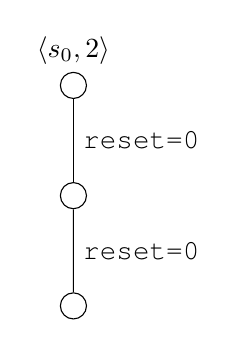
\begin{tikzpicture}[sibling distance = 18mm, level distance = 14mm]
            \node [circle,draw] (root){}
                child {node [circle,draw] {}
                    child {node [circle,draw] {}
                        edge from parent node [right] {\texttt{reset=0}}
                    }
                    edge from parent node [right] {\texttt{reset=0}}
                }
                node [above=4pt] {$\langle s_0, 2 \rangle$};
        \end{tikzpicture}
        \caption{No reset candidate}
        \label{fig:limitationAGTa}
    \end{subfigure}
    \begin{subfigure}[t]{0.5\textwidth}
        \centering
        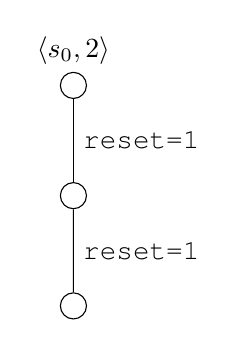
\begin{tikzpicture}[sibling distance = 18mm, level distance = 14mm]
            \node [circle,draw] (root){}
                child {node [circle,draw] {}
                    child {node [circle,draw] {}
                        edge from parent node [right] {\texttt{reset=1}}
                    }
                    edge from parent node [right] {\texttt{reset=1}}
                }
                node [above=4pt] {$\langle s_0, 2 \rangle$};
        \end{tikzpicture}
        \caption{Reset candidate}
        \label{fig:limitationAGTb}
    \end{subfigure}
    \caption{Game trees for the counter specification}
    \label{fig:limitationAGT}
\end{figure}

\subsection{Strengths}

The strength of unbounded synthesis lies in the ability to approximate the winning region. This can be seen on a scaled up version of the example used in Section~\ref{sec:unboundedAlgorithm}. A system with $n$ resources and an environment that can make $m$ requests at once is always realisable if $n \geq m$ by a controller that always grants access to $m$ resources. The problem for BDD solvers is that it can be difficult to compactly represent all $^n C_m$ combinations of granted resources that make up the winning region. With unbounded synthesis a fixed point can be reached by choosing just one winning combination and proving that the environment cannot force an escape from that small set of states.

In Chapter~\ref{ch:bounded} I showed that the strength of the bounded realisability algorithm lies in quickly discovering counterexamples that are difficult to find by representing the entire winning or losing region as a BDD. Unbounded synthesis has similar advantages except that we can extend this advantage to specifications that are realisable.

\section{Summary}

I have now shown how to extend bounded realisability to unbounded games by interpolating abstract game trees to learn an overapproximation of the environment's winning region. The resulting algorithm is a sound and complete procedure for realisability that is efficient is certain cases where BDD based methods are not. In the next chapter I will present an implementation of the algorithm and show results.

\begin{itemize}
    \item Chapter~\ref{ch:bounded} introduced bounded realisability, which constructs game trees as abstractions of the game. An optimisation was described that prunes the search tree by learning the set of states that are losing for a particular abstraction. In this chapter states are learned from the same game trees with interpolation.
    \item Learning with interpolants ensures that certain properties are maintained on the losing states. By carefully maintaining invariants using those properties a fixed point in environment losing states can be detected.
    \item The constructed fixed point is an overapproximation of the total set of environment losing states. Unbounded synthesis can be more efficient than BDD solvers in cases where computing the entire set of states is costly.
\end{itemize}


\chapter{Evaluation}
\label{ch:evaluation}

\newcommand{\eva}[0]{\textsc{EvaSolver}\xspace}
\newcommand{\termitesat}[0]{\textsc{TermiteSAT}\xspace}
\newcommand{\ignore}[1]{}

\definecolor{RYB1}{RGB}{238, 46, 47}
\definecolor{RYB2}{RGB}{0, 140, 72}
\definecolor{RYB3}{RGB}{24, 90, 169}
\definecolor{RYB4}{RGB}{244, 125, 35}
\definecolor{RYB5}{RGB}{102, 44, 145}
\definecolor{RYB6}{RGB}{180, 56, 148}

\pgfplotscreateplotcyclelist{plotcolours}{%
{RYB1!80!black, mark options={fill=RYB1,color=RYB1}, mark=pentagon*},
{RYB3!80!black, mark options={fill=RYB3,color=RYB3}, mark=triangle*},
{RYB2!80!black, mark options={fill=RYB2,color=RYB2}, mark=halfsquare*},
{RYB4!80!black, mark options={fill=RYB4,color=RYB4}, mark=diamond*},
{RYB5!80!black, mark options={fill=RYB5,color=RYB5}, mark=halfcircle*},
{RYB6!80!black, mark options={fill=RYB6,color=RYB6}, mark=x}}

\pgfplotsset{
    every axis plot/.append style={line width=0.8pt},
    every axis/.append style={
        axis lines=middle, 
        x label style={at={(axis description cs:0.5,-0.1)},anchor=north},
        y label style={at={(axis description cs:-0.1,.5)},rotate=90,anchor=south},
        legend style={draw=none,cells={anchor=west},anchor=north west,at={(axis description cs:0.05,1)}},
        cycle list name=plotcolours}
}

In this chapter I present benchmarking results for the implementations of each previous chapter. Bounded realisability is implemented in a tool called \eva as joint work between Nina Narodytska and myself. \eva was built in C++ and is based on the source code of \textsc{RAReQS}~\cite{Janota12}. The tool calls out to Glucose~\cite{Audemard09} for SAT solving. Strategy extraction was later added to \eva using PeRIPLO~\cite{Rollini13} to construct interpolants. The implementation also uses cudd~\cite{Somenzi01} to reduce interpolants into cubes via BDDs. I implemented unbounded realisability in a separate open source tool, \termitesat~\cite{TermiteSAT}, which contains a reimplementation of the bounded realisability algorithm. \termitesat is written in Haskell and also uses Glucose for SAT solving, PeRIPLO for interpolant construction, and cudd to reduce interpolants to cubes. \termitesat was submitted to the 2016 synthesis competition and the results are shown below. As part of that submission I added a hybrid mode to \termitesat that runs the unbounded synthesis algorithm in parallel with Simple BDD Solver~\cite{Walker14b}.

\section{Bounded realisability}

The algorithm is evaluated on four families of benchmarks derived from driver synthesis problems. Bounded realisability is only able to prove the absence of counterexample traces up to a certain length for safety games so the tool is instead evaluated on benchmarks formulated as the dual reachability game. \eva solves games in which the controller must \emph{reach} a goal state. The benchmarks are equivalent to unrealisable safety specifications.  Each benchmark models the data path of one of four I/O devices in the abstracted form.  In particular, we model the transmit buffer of an Ethernet adapter, the send queue of a UART serial controller, the command queue of an SPI Flash controller, and the IDE hard disk DMA descriptor list.   Models are parameterised by the size of the corresponding data structure.  Specifications are written in a simple input language based on the NuSMV syntax~\cite{Henzinger03}.   The transition relation of the game is given in the form of variable update functions $s' := f(\mathcal{S}, \mathcal{U}, \mathcal{C})$, one for each state variable $s \in \mathcal{S}$.

We compare our solver against two existing approaches to solving games.  First, we encode input specifications as QBF instances and solve them using two state-of-the-art QBF solvers: \textsc{RAReQS}~\cite{Janota12} and \textsc{depQBF}~\cite{Lonsing10}, having first run them through the bloqqer~\cite{Biere11} preprocessor.  Second, we solve our benchmarks using the Termite~\cite{Walker14} BDD-based solver that uses dynamic variable reordering, variable grouping, transition relation partitioning, and other optimisations. 

Our experiments, summarised in \Cref{fig:uart,fig:ide,fig:spi,fig:ethernet}, show that off-the-shelf QBF solvers are not well-suited for solving games.  Although our algorithm is inspired by \textsc{RAReQS}, we achieve much better performance, since our solver takes into account the structure of the game, rather than treating it as a generic QBF problem.  

\begin{figure}[ht]
    \centering
    \pgfplotsset{width=\textwidth, height=0.5\textheight}
    \begin{tikzpicture}
        \begin{axis}[xmin=0, xmax=50, ymin=0, ymax=4000, xlabel={Instance size ($| \cS |$)}, ylabel={Time (seconds)}]
            \addplot file {data/bench_uart_eva.dat};
            \addplot file {data/bench_uart_termite.dat};
            \addplot file {data/bench_uart_rareqs.dat};
            \addplot file {data/bench_uart_depqbf.dat};
            \legend{EvaSolver,Termite,RAReQS,depQBF}
        \end{axis}
    \end{tikzpicture}
    \caption{UART}
    \label{fig:uart}
\end{figure}

\begin{figure}[hb]
    \centering
    \pgfplotsset{width=\textwidth, height=0.375\textheight}
    \begin{tikzpicture}
        \begin{axis}[xmin=15, xmax=50, ymin=0, ymax=3000, xlabel={Instance size ($| \cS |$)}, ylabel={Time (seconds)}]
            \addplot file {data/bench_ide_eva.dat};
            \addplot file {data/bench_ide_termite.dat};
%%%            \addplot file {data/bench_ide_rareqs.dat};
%%%            \addplot file {data/bench_ide_depqbf.dat};
            \legend{EvaSolver,Termite,RAReQS,depQBF}
        \end{axis}
    \end{tikzpicture}
    \caption{IDE DMA}
    \label{fig:ide}
\end{figure}

\begin{figure}[ht]
    \centering
    \pgfplotsset{width=\textwidth, height=0.375\textheight}
    \begin{tikzpicture}
        \begin{axis}[xmin=0, xmax=100, ymin=0, ymax=3000, xlabel={Instance size ($| \cS |$)}, ylabel={Time (seconds)}]
            \addplot file {data/bench_spi_eva.dat};
            \addplot file {data/bench_spi_termite.dat};
            \addplot file {data/bench_spi_rareqs.dat};
            \addplot file {data/bench_spi_depqbf.dat};
            \legend{EvaSolver,Termite,RAReQS,depQBF}
        \end{axis}
    \end{tikzpicture}
    \caption{SPI}
    \label{fig:spi}
\end{figure}

\begin{figure}[hb]
    \centering
    \pgfplotsset{width=\textwidth, height=0.5\textheight}
    \begin{tikzpicture}
        \begin{axis}[xmin=0, xmax=75, ymin=0, ymax=4000, xlabel={Instance size ($| \cS |$)}, ylabel={Time (seconds)}]
            \addplot file {data/bench_queue_eva.dat};
            \addplot file {data/bench_queue_termite.dat};
            \addplot file {data/bench_queue_rareqs.dat};
            \addplot file {data/bench_queue_depqbf.dat};
            \legend{EvaSolver,Termite,RAReQS,depQBF}
        \end{axis}
    \end{tikzpicture}
    \caption{Ethernet}
    \label{fig:ethernet}
\end{figure}


All four benchmarks have very large sets of winning states.  
Nevertheless, in the UART and IDE benchmarks, Termite is able to 
represent winning states compactly with only a few thousand BDD 
nodes.  It scales well and outperforms \eva on these benchmarks.  
However, in the two other benchmarks, Termite does not find a 
compact BDD-based representation of the winning set.  \eva 
outperforms Termite on these benchmarks as it does not try to 
enumerate all winning states.

{Detailed performance analysis shows that 
abstract game trees generated in our benchmarks had average 
branching factors in the range between $1.03$ and $1.2$, with 
the maximal depth of the trees ranging from $3$ to $58$.  This
confirms the the key premise behind the design of \eva, namely, 
solving real-world synthesis problems requires considering only a 
small number of opponent moves in every state of the game.}  

\clearpage

\section{Strategy extraction}

%%%\eva implements an important optimisation whereby it generates multiple certificate trees for fragments of the original game, which enables computational learning of winning states.  Our strategy generation algorithm is invoked in an online fashion, whenever \eva computes a certificate tree for a fragment.  This results in multiple partial strategies, where each strategy is computed as described in the previous section.  We introduce an additional final step to \eva, which combines partial strategies into a global winning strategy for the original game.

Strategy extraction is evaluated on the same set of driver synthesis benchmarks.  \Cref{fig:uart2,fig:ide2,fig:spi2,fig:ethernet2} sumarise the results.  For each family, we show strategy generation time as a function of the number of state variables in the specification for a selection of the hardest instances of the family solved by \eva.  Specifically, we show the time it took the base realisability solver to determine the winner (the realisability line), as well as the total time taken to solve the game and compute the winning strategy (the total line).


Table~\ref{table:strategyextractionresults} shows a detailed breakdown of experimental results, including the number of state variables for each instance (\textbf{Vars}) and the total time taken by the solver (\textbf{Total(s)}), split between the time used to determine the winner (and generate certificate trees) (\textbf{Base(s)}) and the strategy generation time (\textbf{Strategy(s)}). The \textbf{OH} column shows the overhead of strategy extraction.

Profiling showed that non-negligible overhead was introduced by transferring CNFs from $\eva$'s internal representation to the representation used by the interpolation library.  This overhead can be almost completely eliminated with additional engineering effort.  Hence, I report the effective overhead (\textbf{EffOH}) of strategy extraction if this engineering effort had been done.

The \textbf{Size} column shows the size of the strategy, i.e., the number of $(W,a,k)$ tuples returned by the \textsc{GenLocalStrats} function.  The last three columns report on the use of the PeRIPLO interpolation library in terms of the number of interpolation operations performed by the algorithm when solving the instance, the average and the maximal size of interpolants returned by PeRIPLO.  The size of an interpolant is reported by the size of its corresponding BDD. This conversion is done by the tool as an optimisation to simplify interpolants into cubes.

These results show that strategy generation adds a modest overhead to the base solver.  Effective overheads are about $12\%$ for IDE and SPI, about $35\%$ for Ethernet and about $30\%$ for UART.  Most of this overhead is due to interpolant computation.  Moreover, experiments show that our algorithm scales linearly with the time taken by the base solver to determine the winner.  

\begin{figure}[ht]
    \centering
    \pgfplotsset{width=\textwidth, height=0.5\textheight}
    \begin{tikzpicture}
        \begin{axis}[xmin=10, xmax=40, ymin=0, ymax=4000, xlabel={Instance size ($| \cS |$)}, ylabel={Time (seconds)}]
            \addplot file {data/bench_strat_uart_total.dat};
            \addplot file {data/bench_strat_uart_real.dat};
            \legend{Total,Realisability}
        \end{axis}
    \end{tikzpicture}
    \caption{Strategy Extraction (UART)}
    \label{fig:uart2}
\end{figure}

\begin{figure}[hb]
    \centering
    \pgfplotsset{width=\textwidth, height=0.25\textheight}
    \begin{tikzpicture}
        \begin{axis}[xmin=25, xmax=35, ymin=0, ymax=2000, xlabel={Instance size ($| \cS |$)}, ylabel={Time (seconds)}]
            \addplot file {data/bench_strat_ide_total.dat};
            \addplot file {data/bench_strat_ide_real.dat};
            \legend{Total,Realisability}
        \end{axis}
    \end{tikzpicture}
    \caption{Strategy Extraction (IDE DMA)}
    \label{fig:ide2}
\end{figure}

\begin{figure}[ht]
    \centering
    \pgfplotsset{width=\textwidth, height=0.4375\textheight}
    \begin{tikzpicture}
        \begin{axis}[xmin=0, xmax=140, ymin=0, ymax=3500, xlabel={Instance size ($| \cS |$)}, ylabel={Time (seconds)}]
            \addplot file {data/bench_strat_spi_total.dat};
            \addplot file {data/bench_strat_spi_real.dat};
            \legend{Total,Realisability}
        \end{axis}
    \end{tikzpicture}
    \caption{Strategy Extraction (SPI)}
    \label{fig:spi2}
\end{figure}

\begin{figure}[hb]
    \centering
    \pgfplotsset{width=\textwidth, height=0.25\textheight}
    \begin{tikzpicture}
        \begin{axis}[ xmin=0, xmax=60, ymin=0, ymax=2000, xlabel={Instance size ($| \cS |$)}, ylabel={Time (seconds)}]
            \addplot file {data/bench_strat_ethernet_total.dat};
            \addplot file {data/bench_strat_ethernet_real.dat};
            \legend{Total,Realisability}
        \end{axis}
    \end{tikzpicture}
    \caption{Strategy Extraction (Ethernet)}
    \label{fig:ethernet2}
\end{figure}

\begin{table}[t]
\resizebox{\columnwidth}{!}{%
\begin{tabular}{r r r r r r r r r r}
\textbf{Vars} & \textbf{Total(s)} & \textbf{Base(s)} & \textbf{Strategy(s)} & \textbf{OH} & \textbf{EffOH} & \textbf{Size} & \textbf{INum} & \textbf{IAvg} & \textbf{IMax}  \\

\hline
\multicolumn{10}{c}{IDE benchmark} \\
\hline
26 & 32.62 & 25.42 & 7.20 & 1.28 & 1.16 & 50    & 48 & \ignore{1193} 23     & \ignore{24155} 118   \\
28 & 42.20 & 35.49 & 6.72 & 1.19 & 1.10 & 59    & 52 & \ignore{2489} 27     & \ignore{39384} 119   \\
30 & 60.04 & 51.93 & 8.11 & 1.16 & 1.08 & 92    & 43 & \ignore{72} 17       & \ignore{1583} 148    \\
32 & 115.11 & 107.35 & 7.77 & 1.07 & 1.04 & 60  & 36 & \ignore{18} 14     & \ignore{85} 27       \\
34 & 283.08 & 227.67 & 55.40 & 1.24 & 1.21 & 159& 49 & \ignore{2150} 15 & \ignore{103941} 38   \\
\hline
\multicolumn{10}{c}{SPI benchmark} \\
\hline
15 & 0.35 & 0.26 & 0.09 & 1.36 & 1.26 & 8             & 5   & \ignore{11} 9 & \ignore{21} 9   \\
22 & 0.94 & 0.72 & 0.22 & 1.31 & 1.19 & 15            & 12  & \ignore{10} 10 & \ignore{22} 18  \\
29 & 2.46 & 1.90 & 0.56 & 1.29 & 1.16 & 22            & 17  & \ignore{12} 10 & \ignore{25} 18  \\
36 & 3.56 & 2.91 & 0.65 & 1.22 & 1.11 & 107           & 22  & \ignore{11} 10 & \ignore{22} 18  \\
43 & 9.11 & 7.09 & 2.03 & 1.29 & 1.13 & 166           & 27  & \ignore{11} 10 & \ignore{21} 14  \\
50 & 16.20 & 12.85 & 3.35 & 1.26 & 1.12 & 233         & 32  & \ignore{11} 11 & \ignore{23} 18  \\
57 & 25.00 & 19.86 & 5.14 & 1.26 & 1.12 & 322         & 37  & \ignore{12} 11 & \ignore{21} 18  \\
64 & 38.48 & 31.48 & 7.00 & 1.22 & 1.10 & 416         & 42  & \ignore{12} 11 & \ignore{24} 18  \\
71 & 57.88 & 47.94 & 9.94 & 1.21 & 1.09 & 70          & 47  & \ignore{12} 12 & \ignore{21} 18  \\
78 & 91.51 & 75.02 & 16.49 & 1.22 & 1.10 & 636        & 52  & \ignore{12} 12 & \ignore{22} 19  \\
85 & 141.10 & 116.71 & 24.39 & 1.21 & 1.09 & 773      & 57  & \ignore{13} 12 & \ignore{23} 20  \\
92 & 193.96 & 162.05 & 31.91 & 1.20 & 1.09 & 917      & 62  & \ignore{13} 13 & \ignore{24} 21  \\
99 & 309.44 & 256.88 & 52.55 & 1.20 & 1.09 & 1059     & 67  & \ignore{13} 13 & \ignore{22} 22  \\
106 & 449.49 & 377.48 & 72.00 & 1.19 & 1.09 & 1223    & 72  & \ignore{13} 13 & \ignore{23} 23  \\
113 & 1645.44 & 1543.84 & 101.60 & 1.07 & 1.03 & 117  & 77  & \ignore{14} 13 & \ignore{24} 24  \\
120 & 901.95 & 830.17 & 71.77 & 1.09 & 1.04 & 1637    & 82  & \ignore{14} 14 & \ignore{25} 25  \\
127 & 2259.65 & 2143.40 & 116.25 & 1.05 & 1.02 & 139  & 87  & \ignore{14} 14 & \ignore{26} 26  \\
134 & 2385.74 & 2193.65 & 192.09 & 1.09 & 1.04 & 152  & 92  & \ignore{14} 14 & \ignore{27} 27  \\
\hline
\multicolumn{10}{c}{Ethernet benchmarks} \\
\hline
14 & 0.06 & 0.03 & 0.02 & 1.60 & 1.52 & 2             & 1    & \ignore{24} 13  & \ignore{24} 13    \\
17 & 0.49 & 0.29 & 0.20 & 1.70 & 1.45 & 21            & 7    & \ignore{33} 16  & \ignore{87} 30    \\
20 & 1.97 & 1.14 & 0.82 & 1.72 & 1.45 & 176           & 15   & \ignore{41} 16  & \ignore{110} 26   \\
23 & 5.39 & 3.23 & 2.16 & 1.67 & 1.39 & 185           & 25   & \ignore{64} 23  & \ignore{180} 42   \\
26 & 14.61 & 7.94 & 6.66 & 1.84 & 1.48 & 266          & 36   & \ignore{100} 24 & \ignore{347} 45   \\
29 & 27.41 & 15.71 & 11.70 & 1.74 & 1.43 & 677        & 44   & \ignore{155} 24 & \ignore{779} 48   \\
32 & 58.02 & 35.38 & 22.64 & 1.64 & 1.36 & 208        & 61   & \ignore{136} 28 & \ignore{676} 55   \\
35 & 111.69 & 69.26 & 42.43 & 1.61 & 1.35 & 351       & 80   & \ignore{141} 31 & \ignore{933} 75   \\
38 & 238.09 & 151.21 & 86.89 & 1.57 & 1.33 & 545      & 116  & \ignore{184} 32 & \ignore{1081} 63  \\
41 & 513.61 & 321.78 & 191.82 & 1.60 & 1.34 & 1525    & 154  & \ignore{184} 35 & \ignore{1123} 72  \\
44 & 845.51 & 530.68 & 314.83 & 1.59 & 1.34 & 2159    & 191  & \ignore{276} 37 & \ignore{2253} 64  \\
47 & 903.79 & 590.19 & 313.60 & 1.53 & 1.30 & 1547    & 228  & \ignore{261} 38 & \ignore{1780} 71  \\
50 & 1368.23 & 875.90 & 492.33 & 1.56 & 1.33 & 1670   & 236  & \ignore{372} 38 & \ignore{2292} 85  \\
\hline
\multicolumn{10}{c}{UART benchmarks} \\
\hline
15 & 2.86 & 2.19 & 0.67 & 1.31 & 1.19 & 12             & 40  & \ignore{28} 6   & \ignore{90} 14    \\
20 & 3.16 & 2.33 & 0.83 & 1.36 & 1.20 & 20             & 14  & \ignore{35} 12  & \ignore{155} 23   \\
21 & 10.06 & 6.96 & 3.09 & 1.44 & 1.24 & 35            & 34  & \ignore{48} 9   & \ignore{306} 26   \\
26 & 27.89 & 18.55 & 9.34 & 1.50 & 1.27 & 65           & 60  & \ignore{92} 13  & \ignore{730} 41   \\
27 & 63.68 & 41.49 & 22.20 & 1.53 & 1.29 & 93          & 94  & \ignore{96} 13  & \ignore{825} 44   \\
28 & 137.24 & 90.68 & 46.56 & 1.51 & 1.27 & 103        & 136 & \ignore{138} 13 & \ignore{1356} 42   \\
29 & 270.66 & 178.75 & 91.92 & 1.51 & 1.27 & 134       & 184 & \ignore{212} 15 & \ignore{2806} 47   \\
34 & 553.29 & 360.76 & 192.53 & 1.53 & 1.28 & 191      & 246 & \ignore{299} 16 & \ignore{6360} 54   \\
35 & 938.68 & 612.63 & 326.05 & 1.53 & 1.28 & 285      & 307 & \ignore{258} 16 & \ignore{7949} 69   \\
36 & 1525.99 & 995.25 & 530.74 & 1.53 & 1.28 & 410     & 382 & \ignore{348} 17 & \ignore{6408} 62   \\
37 & 2464.13 & 1611.45 & 852.68 & 1.53 & 1.28 & 950    & 456 & \ignore{414} 18 & \ignore{10592} 75  \\
38 & 3927.64 & 2577.39 & 1350.25 & 1.52 & 1.28 & 1223  & 546 & \ignore{504} 18 & \ignore{34431} 74  \\
39 & 6030.77 & 4031.98 & 1998.79 & 1.50 & 1.26 & 674   & 633 & \ignore{608} 18 & \ignore{29996} 72  \\
\hline
\end{tabular}}
\caption{Detailed strategy extraction results}
\label{table:strategyextractionresults}
\end{table}


%%%These results show that strategy extraction is efficient, scalable and robust.  The last property is particularly interesting, as existing strategy extraction algorithms for traditional game solvers, based on winning set compilation, have been reported to introduce significant variance across instances~\cite{Bloem_KS_14corr,Bloem_KS_13}.  A conclusive comparison can only be performed by evaluating both types of algorithms on a common set of benchmarks.  Such a comparison requires first extending $\eva$ to support unbounded safety and reachability games and is part of the future work.

\clearpage

\section{Unbounded realisability}

Unbounded realisability is evaluated on the benchmarks of the 2015 synthesis competition (SYNTCOMP'15). I also show the results of the 2016 competition, which \termitesat was submitted to. Each competition benchmark comprises of controllable and uncontrollable inputs to a circuit that assigns values to latches. One latch is configured as the error bit that determines the winner of the safety game. The benchmark suite is a collection of both real-world and toy specifications including generalised buffers, AMBA bus controllers, device drivers, and converted LTL formulas.  Descriptions of many of the benchmark families used can be found in the 2014 competition report~\cite{Jacobs15}. 

\subsection{Benchmarking}

The benchmarks were run on a cluster of Intel Quad Core Xeon E5405 2GHz CPUs with 16GB of memory.  The solvers were allowed exclusive access to a node for one hour to solve an instance.  The results of this benchmarking are shown, along with the synthesis competition results~\cite{syntcompedacc}, in Table~\ref{tab:syntcomp}. The competition was run on Intel Quad Core 3.2Ghz CPUs with 32GB of memory, also on isolated nodes for one hour per instance. The competition results differ significantly from our own benchmarks due to this more powerful hardware.  For our benchmarks we report only the results for solvers we were able to run on our cluster. The unique column lists the number of instances that only that tool could solve in the competition (excluding our solver). In brackets is the number of instances that only that tool could solve, including our solver.

\begin{table}[b]
    \centering
    \setlength{\tabcolsep}{8pt}
    \begin{tabular}{l | r | r | r }
        \textbf{Solver} & \textbf{Solved} & \textbf{Solved} & \textbf{Unique} \\
                        & \textbf{(Competition)} & \textbf{(Benchmarks)} & \\
        \hline
        Simple BDD Solver (2) & 195 & 189 & 10 \textit{(6)} \\
        AbsSynthe (seq2) & 187 & 139 & 2 \\
        Simple BDD Solver (1) & 185 & 175 & \\
        AbsSynthe (seq3) & 179 & 134 & \\
        Realizer (sequential) & 179 & & \\
        AbsSynthe (seq1) & 173 & 139 & 1 \\
        Demiurge (D1real) & 139 & 136 & 5 \textit{(2)} \\
        Aisy & 98 & \\
        \textit{Unbounded Synthesis} & & \textit{103} & \textit{12} \\
    \end{tabular}
    \caption{Synthesis Competition 2015 Results}
    \label{tab:syntcomp}
\end{table}

Our implementation was able to solve 103 out of the 250 specification in the alloted time, including 12 instances that were not solved by any other solver in the sequential track of the competition. The unique instances we solved are listed in Table~\ref{tab:unique}.

\begin{table}[h]
    \centering
    \setlength{\tabcolsep}{16pt}
    \begin{tabular}{l l}
        1. \texttt{6s216rb0\_c0to31} & 7. \texttt{driver\_c10n} \\
        2. \texttt{cnt30y} &  8. \texttt{stay18y} \\
        3. \texttt{driver\_a10n} & 9. \texttt{stay20n} \\
        4. \texttt{driver\_a8n} & 10. \texttt{stay20y} \\
        5. \texttt{driver\_b10y} & 11. \texttt{stay22n} \\
        6. \texttt{driver\_b8y} & 12. \texttt{stay22y} \\
    \end{tabular}
    \caption{Instances uniquely solved by our approach}
    \label{tab:unique}
\end{table}

Five of the instances unique to our solver are device driver instances and another five are from the \texttt{stay} family. This supports the hypothesis that different game solving methodologies perform better on certain classes of specifications.

I also present a cactus plot of the number of instances solved over time (Figure~\ref{fig:cactus}). We have plotted the best configuration of each solver we benchmarked. The solvers shown are \textsc{Demiurge}~\cite{Bloem14}, the only SAT-based tool in the competition, the winner of the sequential realisability track \textsc{Simple BDD Solver 2}~\cite{Walker14}, and AbsSynthe (seq3) \cite{Brenguier14}.

\begin{figure}
    \centering
    \pgfplotsset{width=\textwidth}
    \begin{tikzpicture}
        \begin{axis}[ xmin=0, xmax=60, ymin=0, ymax=200, xlabel={Time (minutes)}, ylabel={Instances solved},
                legend style={draw=none,cells={anchor=west},anchor=south east,at={(axis description cs:1,0.05)}}]
            \addplot file {data/bench_termite.dat};
            \addplot file {data/bench_demiurge.dat};
            \addplot file {data/bench_simple2.dat};
            \addplot file {data/bench_abs1.dat};
            \legend{TermiteSAT,Demiurge,Simple BDD Solver,AbsSynthe}
        \end{axis}
    \end{tikzpicture}
    \caption{Number of instances solved over time.}
    \label{fig:cactus}
\end{figure}

%%%Whilst our solver is unable to solve as many instances as other tools, it was
%%%able to solve more unique instances than any solver in the competition. This
%%%confirms that our methodology is able to fill gaps in a state of the art
%%%synthesis toolbox by more efficiently solving instances that are hard for other
%%%techniques. For this reason our solver would be a worthwhile addition to a
%%%portfolio solver. In the parallel track of the competition, \textsc{Demiurge}
%%%uses a suite of 3 separate but communicating solvers. The solvers
%%%relay unsafe states to one another, which is compatible with the set $B^M$ in
%%%our solver. This technique can already solve each of the unique instances
%%%solved by our solver but there may still be value in the addition of this work
%%%to the portfolio.  It remains future work to explore this possibility.

\subsection{Synthesis Competition Results}

I report the results of the sequential realisability track of the 2016 synthesis competition in Table~\ref{table:syntcomp16s}

\begin{table}

    \caption{SYNTCOMP'16 sequential realisability track}
    \label{table:syntcomp16s}
\end{table}

\begin{figure}
    \centering
    \pgfplotsset{width=\textwidth}
    \begin{tikzpicture}
        \begin{axis}[ xmin=0, xmax=60, ymin=0, ymax=200, xlabel={Time (minutes)}, ylabel={Instances solved},
                legend style={draw=none,cells={anchor=west},anchor=south east,at={(axis description cs:1,0.05)}}]
            \addplot file {data/comp_sequential_TermiteSAT.dat};
            \addplot file {data/comp_sequential_SimpleBDDSolverwithAbstraction.dat};
            \addplot file {data/comp_sequential_DemiurgeD1real.dat};
            \addplot file {data/comp_sequential_AbsSyntheS3.dat};
            \addplot file {data/comp_sequential_SafetySynth.dat};
            \addplot file {data/comp_sequential_SDF.dat};
            \legend{TermiteSAT,Demiurge,Simple BDD Solver,AbsSynthe,SafetySynth,SDF}
        \end{axis}
    \end{tikzpicture}
    \caption{SYNTCOMP'16 sequential track: Instances solved over time}
    \label{fig:syntcomp16seq}
\end{figure}


\section{Summary}


\chapter{Conclusion}
\label{ch:conclusion}

Controller synthesis may one day become the tool of choice for designers of reactive systems. As an approach to software correctness its advantages are clear but the future of synthesis is held back by computational complexity. In this thesis I presented a technique that takes one small step towards feasibility by focussing on a particular class of specifications.

The basis of this methodology is a counterexample guided bounded realisability algorithm. The algorithm constructs abstractions of the safety game and existentially searches for player strategies. The approach is similar to existing QBF methodologies but is able to perform better than those by taking advantage of knowledge of the structure of the problem. I also presented an algorithm to extract the strategy from the certificate generated during bounded realisability. Additionally I presented an approach that extends the algorithm to solve unbounded games. The complete synthesis algorithm is suited to safety specifications where the winning region has no compact representation as a binary decision diagram.


\backmatter
\cleardoublepage
\listoffigures
\cleardoublepage
\bibliographystyle{thesisnat}
\bibliography{main}

\end{document}
